% Generated by Sphinx.
\def\sphinxdocclass{report}
\documentclass[letterpaper,10pt,english]{sphinxmanual}
\usepackage[utf8]{inputenc}
\DeclareUnicodeCharacter{00A0}{\nobreakspace}
\usepackage[T1]{fontenc}
\usepackage{babel}
\usepackage{times}
\usepackage[Bjarne]{fncychap}
\usepackage{longtable}
\usepackage{sphinx}
\usepackage{multirow}


\title{pyGPs API}
\date{July 08, 2014}
\release{v1.2}
\author{M. Neumann, S. Huang, D. Marthaler, K. Kersting}
\newcommand{\sphinxlogo}{}
\renewcommand{\releasename}{Release}
\makeindex

\makeatletter
\def\PYG@reset{\let\PYG@it=\relax \let\PYG@bf=\relax%
    \let\PYG@ul=\relax \let\PYG@tc=\relax%
    \let\PYG@bc=\relax \let\PYG@ff=\relax}
\def\PYG@tok#1{\csname PYG@tok@#1\endcsname}
\def\PYG@toks#1+{\ifx\relax#1\empty\else%
    \PYG@tok{#1}\expandafter\PYG@toks\fi}
\def\PYG@do#1{\PYG@bc{\PYG@tc{\PYG@ul{%
    \PYG@it{\PYG@bf{\PYG@ff{#1}}}}}}}
\def\PYG#1#2{\PYG@reset\PYG@toks#1+\relax+\PYG@do{#2}}

\def\PYG@tok@gd{\def\PYG@tc##1{\textcolor[rgb]{0.63,0.00,0.00}{##1}}}
\def\PYG@tok@gu{\let\PYG@bf=\textbf\def\PYG@tc##1{\textcolor[rgb]{0.50,0.00,0.50}{##1}}}
\def\PYG@tok@gt{\def\PYG@tc##1{\textcolor[rgb]{0.00,0.25,0.82}{##1}}}
\def\PYG@tok@gs{\let\PYG@bf=\textbf}
\def\PYG@tok@gr{\def\PYG@tc##1{\textcolor[rgb]{1.00,0.00,0.00}{##1}}}
\def\PYG@tok@cm{\let\PYG@it=\textit\def\PYG@tc##1{\textcolor[rgb]{0.25,0.50,0.56}{##1}}}
\def\PYG@tok@vg{\def\PYG@tc##1{\textcolor[rgb]{0.73,0.38,0.84}{##1}}}
\def\PYG@tok@m{\def\PYG@tc##1{\textcolor[rgb]{0.13,0.50,0.31}{##1}}}
\def\PYG@tok@mh{\def\PYG@tc##1{\textcolor[rgb]{0.13,0.50,0.31}{##1}}}
\def\PYG@tok@cs{\def\PYG@tc##1{\textcolor[rgb]{0.25,0.50,0.56}{##1}}\def\PYG@bc##1{\colorbox[rgb]{1.00,0.94,0.94}{##1}}}
\def\PYG@tok@ge{\let\PYG@it=\textit}
\def\PYG@tok@vc{\def\PYG@tc##1{\textcolor[rgb]{0.73,0.38,0.84}{##1}}}
\def\PYG@tok@il{\def\PYG@tc##1{\textcolor[rgb]{0.13,0.50,0.31}{##1}}}
\def\PYG@tok@go{\def\PYG@tc##1{\textcolor[rgb]{0.19,0.19,0.19}{##1}}}
\def\PYG@tok@cp{\def\PYG@tc##1{\textcolor[rgb]{0.00,0.44,0.13}{##1}}}
\def\PYG@tok@gi{\def\PYG@tc##1{\textcolor[rgb]{0.00,0.63,0.00}{##1}}}
\def\PYG@tok@gh{\let\PYG@bf=\textbf\def\PYG@tc##1{\textcolor[rgb]{0.00,0.00,0.50}{##1}}}
\def\PYG@tok@ni{\let\PYG@bf=\textbf\def\PYG@tc##1{\textcolor[rgb]{0.84,0.33,0.22}{##1}}}
\def\PYG@tok@nl{\let\PYG@bf=\textbf\def\PYG@tc##1{\textcolor[rgb]{0.00,0.13,0.44}{##1}}}
\def\PYG@tok@nn{\let\PYG@bf=\textbf\def\PYG@tc##1{\textcolor[rgb]{0.05,0.52,0.71}{##1}}}
\def\PYG@tok@no{\def\PYG@tc##1{\textcolor[rgb]{0.38,0.68,0.84}{##1}}}
\def\PYG@tok@na{\def\PYG@tc##1{\textcolor[rgb]{0.25,0.44,0.63}{##1}}}
\def\PYG@tok@nb{\def\PYG@tc##1{\textcolor[rgb]{0.00,0.44,0.13}{##1}}}
\def\PYG@tok@nc{\let\PYG@bf=\textbf\def\PYG@tc##1{\textcolor[rgb]{0.05,0.52,0.71}{##1}}}
\def\PYG@tok@nd{\let\PYG@bf=\textbf\def\PYG@tc##1{\textcolor[rgb]{0.33,0.33,0.33}{##1}}}
\def\PYG@tok@ne{\def\PYG@tc##1{\textcolor[rgb]{0.00,0.44,0.13}{##1}}}
\def\PYG@tok@nf{\def\PYG@tc##1{\textcolor[rgb]{0.02,0.16,0.49}{##1}}}
\def\PYG@tok@si{\let\PYG@it=\textit\def\PYG@tc##1{\textcolor[rgb]{0.44,0.63,0.82}{##1}}}
\def\PYG@tok@s2{\def\PYG@tc##1{\textcolor[rgb]{0.25,0.44,0.63}{##1}}}
\def\PYG@tok@vi{\def\PYG@tc##1{\textcolor[rgb]{0.73,0.38,0.84}{##1}}}
\def\PYG@tok@nt{\let\PYG@bf=\textbf\def\PYG@tc##1{\textcolor[rgb]{0.02,0.16,0.45}{##1}}}
\def\PYG@tok@nv{\def\PYG@tc##1{\textcolor[rgb]{0.73,0.38,0.84}{##1}}}
\def\PYG@tok@s1{\def\PYG@tc##1{\textcolor[rgb]{0.25,0.44,0.63}{##1}}}
\def\PYG@tok@gp{\let\PYG@bf=\textbf\def\PYG@tc##1{\textcolor[rgb]{0.78,0.36,0.04}{##1}}}
\def\PYG@tok@sh{\def\PYG@tc##1{\textcolor[rgb]{0.25,0.44,0.63}{##1}}}
\def\PYG@tok@ow{\let\PYG@bf=\textbf\def\PYG@tc##1{\textcolor[rgb]{0.00,0.44,0.13}{##1}}}
\def\PYG@tok@sx{\def\PYG@tc##1{\textcolor[rgb]{0.78,0.36,0.04}{##1}}}
\def\PYG@tok@bp{\def\PYG@tc##1{\textcolor[rgb]{0.00,0.44,0.13}{##1}}}
\def\PYG@tok@c1{\let\PYG@it=\textit\def\PYG@tc##1{\textcolor[rgb]{0.25,0.50,0.56}{##1}}}
\def\PYG@tok@kc{\let\PYG@bf=\textbf\def\PYG@tc##1{\textcolor[rgb]{0.00,0.44,0.13}{##1}}}
\def\PYG@tok@c{\let\PYG@it=\textit\def\PYG@tc##1{\textcolor[rgb]{0.25,0.50,0.56}{##1}}}
\def\PYG@tok@mf{\def\PYG@tc##1{\textcolor[rgb]{0.13,0.50,0.31}{##1}}}
\def\PYG@tok@err{\def\PYG@bc##1{\fcolorbox[rgb]{1.00,0.00,0.00}{1,1,1}{##1}}}
\def\PYG@tok@kd{\let\PYG@bf=\textbf\def\PYG@tc##1{\textcolor[rgb]{0.00,0.44,0.13}{##1}}}
\def\PYG@tok@ss{\def\PYG@tc##1{\textcolor[rgb]{0.32,0.47,0.09}{##1}}}
\def\PYG@tok@sr{\def\PYG@tc##1{\textcolor[rgb]{0.14,0.33,0.53}{##1}}}
\def\PYG@tok@mo{\def\PYG@tc##1{\textcolor[rgb]{0.13,0.50,0.31}{##1}}}
\def\PYG@tok@mi{\def\PYG@tc##1{\textcolor[rgb]{0.13,0.50,0.31}{##1}}}
\def\PYG@tok@kn{\let\PYG@bf=\textbf\def\PYG@tc##1{\textcolor[rgb]{0.00,0.44,0.13}{##1}}}
\def\PYG@tok@o{\def\PYG@tc##1{\textcolor[rgb]{0.40,0.40,0.40}{##1}}}
\def\PYG@tok@kr{\let\PYG@bf=\textbf\def\PYG@tc##1{\textcolor[rgb]{0.00,0.44,0.13}{##1}}}
\def\PYG@tok@s{\def\PYG@tc##1{\textcolor[rgb]{0.25,0.44,0.63}{##1}}}
\def\PYG@tok@kp{\def\PYG@tc##1{\textcolor[rgb]{0.00,0.44,0.13}{##1}}}
\def\PYG@tok@w{\def\PYG@tc##1{\textcolor[rgb]{0.73,0.73,0.73}{##1}}}
\def\PYG@tok@kt{\def\PYG@tc##1{\textcolor[rgb]{0.56,0.13,0.00}{##1}}}
\def\PYG@tok@sc{\def\PYG@tc##1{\textcolor[rgb]{0.25,0.44,0.63}{##1}}}
\def\PYG@tok@sb{\def\PYG@tc##1{\textcolor[rgb]{0.25,0.44,0.63}{##1}}}
\def\PYG@tok@k{\let\PYG@bf=\textbf\def\PYG@tc##1{\textcolor[rgb]{0.00,0.44,0.13}{##1}}}
\def\PYG@tok@se{\let\PYG@bf=\textbf\def\PYG@tc##1{\textcolor[rgb]{0.25,0.44,0.63}{##1}}}
\def\PYG@tok@sd{\let\PYG@it=\textit\def\PYG@tc##1{\textcolor[rgb]{0.25,0.44,0.63}{##1}}}

\def\PYGZbs{\char`\\}
\def\PYGZus{\char`\_}
\def\PYGZob{\char`\{}
\def\PYGZcb{\char`\}}
\def\PYGZca{\char`\^}
\def\PYGZsh{\char`\#}
\def\PYGZpc{\char`\%}
\def\PYGZdl{\char`\$}
\def\PYGZti{\char`\~}
% for compatibility with earlier versions
\def\PYGZat{@}
\def\PYGZlb{[}
\def\PYGZrb{]}
\makeatother

\begin{document}

\maketitle
\tableofcontents
\phantomsection\label{index::doc}



\chapter{pyGPs - A Package for Gaussian Processes}
\label{index:pygps-a-package-for-gaussian-processes}\label{index:welcome-to-pygps-s-api}

\section{About the package}
\label{index:about-the-package}
pyGPs is a library hosting Python implementations of Gaussian processes (GPs) for
machine learning.
pyGPs bridges the gap between systems designed primarily for users, who mainly
want to apply GPs and need basic machine learning routines for model training, evaluation, and
visualiztion, and expressive systems for developers, who focus on extending the core
functionalities as covariance and likelihood functions, as well as inference techniques.

The software package is released under the BSD 2-Clause (FreeBSD) License.
\code{Copyright} (c) by
Marion Neumann, Shan Huang, Daniel Marthaler, \& Kristian Kersting, Feb.2014

Further, it includes implementations of
\begin{itemize}
\item {} 
minimize.py implemented in python by Roland Memisevic 2008, following minimize.m (Copyright (c) Carl Edward Rasmussen (1999-2006))

\item {} 
scg.py (Copyright (c) Ian T Nabney (1996-2001))

\item {} 
brentmin.py (Copyright (c) Hannes Nickisch 2010-01-10)

\item {} 
FITC functionality (following matlab implementations under Copyright (c) by Ed Snelson, Carl Edward Rasmussen and Hannes Nickisch, 2011-11-02)

\end{itemize}

The most recent stable release is pyGPs v1.2. If you observe problems or bugs, please let us know.
You can also download a \href{https://github.com/marionmari/pyGP\_PR/}{procedual implementation} of GP functionality from Github. However, the procedual version will not be supported in future.
\begin{description}
\item[{Authors:}] \leavevmode\begin{itemize}
\item {} 
Marion Neumann {[}marion dot neumann at uni-bonn dot de{]}

\item {} 
Shan Huang {[}shan dot huang at iais dot fraunhofer dot de{]}

\item {} 
Daniel Marthaler {[}marthaler at ge dot com{]}

\item {} 
Kristian Kersting {[}kristian dot kersting at cs dot tu-dortmund dot de{]}

\end{itemize}

\end{description}

The following persons helped to improve this software: Roman Garnett, Maciej Kurek, Hannes Nickisch, Zhao Xu, and Alejandro Molina.

This work is partly supported by the Fraunhofer ATTRACT fellowship STREAM.


\section{Getting started}
\label{index:getting-started}

\subsection{Installation}
\label{Install:installation}\label{Install::doc}\begin{enumerate}
\item {} 
First, \href{https://github.com/marionmari/pyGPs/releases/tag/v1.1}{download} the archive from github and extract it to any local directory.

\end{enumerate}
\begin{enumerate}
\setcounter{enumi}{1}
\item {} 
You can either add the local directory to your PYTHONPATH

\begin{Verbatim}[commandchars=\\\{\}]
export PYTHONPATH=\$PYTHONPATH:/path/to/local/directory/../parent\_folder\_of\_pyGPs
\end{Verbatim}

\item {} 
Or install the package using setup.py:

\begin{Verbatim}[commandchars=\\\{\}]
sudo python setup.py install
\end{Verbatim}

\end{enumerate}


\subsubsection{Requirements}
\label{Install:requirements}\begin{itemize}
\item {} 
\href{http://www.python.org/}{python 2.6 or 2.7}

\item {} 
\href{http://www.scipy.org/}{scipy}, \href{http://www.numpy.org/}{numpy}, and \href{http://matplotlib.org/}{matplotlib}: open-source packages for scientific computing in Python.

\end{itemize}

Example installation on Ubuntu \& Debian:

\begin{Verbatim}[commandchars=\\\{\}]
sudo apt-get install python2.7 python-numpy python-scipy python-matplotlib
\end{Verbatim}

Example installation on Mac via Macports (requires XCode and MacPorts):

\begin{Verbatim}[commandchars=\\\{\}]
sudo port install python27 py27-numpy py27-scipy py27-matplotlib
\end{Verbatim}

For other systems please check the installation instructions on the respective package web sites.


\subsection{GPs \& Functionality}
\label{Theory:gps-functionality}\label{Theory::doc}
Gaussian Processes (GPs) can conveniently be used for Bayesian supervised learning, such as regression and classification.
In its simplest form, GP inference can be implemented in a few lines of code. However, in practice, things typically
get a little more complicated: you might want to use expressive covariance and mean functions, learn good values
for hyperparameters, use non-Gaussian likelihood functions (rendering exact inference intractable), use approximate inference
algorithms, or combinations of many or all of the above.

A comprehensive introduction to Gaussian Processes for Machine Learning is provided in the \href{http://www.gaussianprocess.org/gpml}{GPML} book by Rasmussen and Williams, 2006.


\section{Tutorials}
\label{index:tutorials}\label{index:gpml}

\subsection{Demos}
\label{Examples:demos}\label{Examples::doc}
There are several demos exemplifying the use of pyGPs for various Gaussian process ($GP$) tasks.
We recommend to first go through \emph{Basic GP Regression} which introduces the $GP$ regression model.
Basic regression is the most intuitive and simplest learning task feasable with $GPs$.
The other demos will then provide a general insight into more advanced functionalities of the package.
You will also find the implementation of the demos in the \href{https://github.com/marionmari/pyGPs}{source} folder under \href{https://github.com/marionmari/pyGPs/tree/master/pyGPs/Demo}{pyGPs/Demo}.

The Demos give some theoretical explanations. Further, it is useful to have a look at our documentation on Kernels \& Means and Optimizers.

Regression


\subsubsection{Basic Regression}
\label{GPR:basic-regression}\label{GPR::doc}
The code shown in this tutorial can be executed by running \emph{pyGPs/Demo/demo\_GPR.py}

This demo will not only introduce the regression model, it also provides the general insight of how to use the package. This general information will not be repeated in the other demos.


\paragraph{Import packages}
\label{GPR:import-packages}
Once you installed pyGPs, the typical way to import it is:

\begin{Verbatim}[commandchars=\\\{\}]
\PYG{k+kn}{from} \PYG{n+nn}{pyGPs.Core} \PYG{k+kn}{import} \PYG{o}{*}
\PYG{k+kn}{import} \PYG{n+nn}{numpy} \PYG{k+kn}{as} \PYG{n+nn}{np}
\end{Verbatim}


\paragraph{Load data}
\label{GPR:load-data}
First, load the data for this demo. The data consists of $n=20$ 1-d data points drawn from a unit Gaussian. This is the same data used in the GPML example (it is hardcoded in \emph{data/regression\_data.npz}).

\begin{Verbatim}[commandchars=\\\{\}]
\PYG{n}{demoData} \PYG{o}{=} \PYG{n}{np}\PYG{o}{.}\PYG{n}{load}\PYG{p}{(}\PYG{l+s}{'}\PYG{l+s}{data\PYGZus{}for\PYGZus{}demo/regression\PYGZus{}data.npz}\PYG{l+s}{'}\PYG{p}{)}
\PYG{n}{x} \PYG{o}{=} \PYG{n}{demoData}\PYG{p}{[}\PYG{l+s}{'}\PYG{l+s}{x}\PYG{l+s}{'}\PYG{p}{]}      \PYG{c}{\PYGZsh{} training data}
\PYG{n}{y} \PYG{o}{=} \PYG{n}{demoData}\PYG{p}{[}\PYG{l+s}{'}\PYG{l+s}{y}\PYG{l+s}{'}\PYG{p}{]}      \PYG{c}{\PYGZsh{} training target}
\PYG{n}{z} \PYG{o}{=} \PYG{n}{demoData}\PYG{p}{[}\PYG{l+s}{'}\PYG{l+s}{xstar}\PYG{l+s}{'}\PYG{p}{]}  \PYG{c}{\PYGZsh{} test data}
\end{Verbatim}


\paragraph{A five-line toy example}
\label{GPR:a-five-line-toy-example}
Now lets do regression with Gaussian processes.
Using pyGPs for regression is really simple; here is the most basic example:

\begin{Verbatim}[commandchars=\\\{\}]
\PYG{n}{model} \PYG{o}{=} \PYG{n}{gp}\PYG{o}{.}\PYG{n}{GPR}\PYG{p}{(}\PYG{p}{)}    \PYG{c}{\PYGZsh{} specify model (GP regression)}
\PYG{n}{model}\PYG{o}{.}\PYG{n}{fit}\PYG{p}{(}\PYG{n}{x}\PYG{p}{,} \PYG{n}{y}\PYG{p}{)}     \PYG{c}{\PYGZsh{} fit default model (mean zero \& rbf kernel) with data}
\PYG{n}{model}\PYG{o}{.}\PYG{n}{train}\PYG{p}{(}\PYG{n}{x}\PYG{p}{,} \PYG{n}{y}\PYG{p}{)}   \PYG{c}{\PYGZsh{} optimize hyperparamters (default optimizer: single run minimize)}
\PYG{n}{model}\PYG{o}{.}\PYG{n}{predict}\PYG{p}{(}\PYG{n}{z}\PYG{p}{)}    \PYG{c}{\PYGZsh{} predict test cases}
\PYG{n}{model}\PYG{o}{.}\PYG{n}{plot}\PYG{p}{(}\PYG{p}{)}        \PYG{c}{\PYGZsh{} and plot result}
\end{Verbatim}

By default, GPR uses a zero mean, the rbf kernel and a Gaussian likelihood. Default optimizer is a single run of Rasmussen's minimize. You will see below how to set non-default values in another example.

\emph{GPR.plot()} will plot the result, where the dark line is the posterior mean and the green-shaded area is the posterior variance.
Note, that \emph{plot()} is not a general method as it is not trivial to visualize high dimensional data.
Here, \emph{GPR.plot()} works for 1-d data only, while \emph{GPC.plot()} is a toy method visualising 2-d input data in a classification scenario.
\begin{figure}[htbp]
\centering

\scalebox{0.700000}{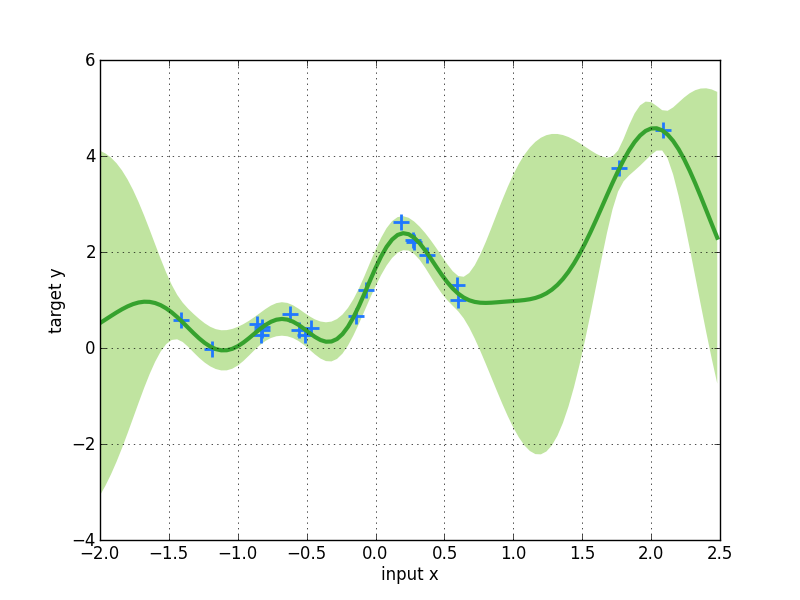
\includegraphics{_images/d1_1.png}}
\end{figure}


\paragraph{A more complicated example}
\label{GPR:a-more-complicated-example}
Now lets do another example to get insight into more advanced features of the toolbox.

You can specify non-default mean and covariance functions:

\begin{Verbatim}[commandchars=\\\{\}]
\PYG{n}{m} \PYG{o}{=} \PYG{n}{mean}\PYG{o}{.}\PYG{n}{Linear}\PYG{p}{(} \PYG{n}{D}\PYG{o}{=}\PYG{n}{x}\PYG{o}{.}\PYG{n}{shape}\PYG{p}{[}\PYG{l+m+mi}{1}\PYG{p}{]} \PYG{p}{)} \PYG{o}{+} \PYG{n}{mean}\PYG{o}{.}\PYG{n}{Const}\PYG{p}{(}\PYG{p}{)}
\PYG{n}{k} \PYG{o}{=} \PYG{n}{cov}\PYG{o}{.}\PYG{n}{RBF}\PYG{p}{(}\PYG{p}{)}
\PYG{n}{model}\PYG{o}{.}\PYG{n}{setPrior}\PYG{p}{(}\PYG{n}{mean}\PYG{o}{=}\PYG{n}{m}\PYG{p}{,} \PYG{n}{kernel}\PYG{o}{=}\PYG{n}{k}\PYG{p}{)}
\end{Verbatim}

Here, we use a composite mean as the sum of a linear and a constant function, and an rbf kernel. The initial hyperparameters are left to their default values. See Kernels \& Means for a complete documentation of kernel/mean specification and custom kernel/mean construction. Once kernel and mean are specified, they are passed to the prior using \emph{setPrior()}.

You can add the traning data to the model explicitly by using \emph{setData()}. So, you avoid passing them into \emph{fit()} or \emph{train()} each time used. More importantly, the deafult mean will be adapted to the average value of the trainging labels $y$ (if you do not specify mean function by your own).

Further, you can plot the data in the 1-d case:

\begin{Verbatim}[commandchars=\\\{\}]
\PYG{n}{model}\PYG{o}{.}\PYG{n}{setData}\PYG{p}{(}\PYG{n}{x}\PYG{p}{,} \PYG{n}{y}\PYG{p}{)}
\PYG{n}{model}\PYG{o}{.}\PYG{n}{plotData\PYGZus{}1d}\PYG{p}{(}\PYG{p}{)}
\end{Verbatim}
\begin{figure}[htbp]
\centering

\scalebox{0.700000}{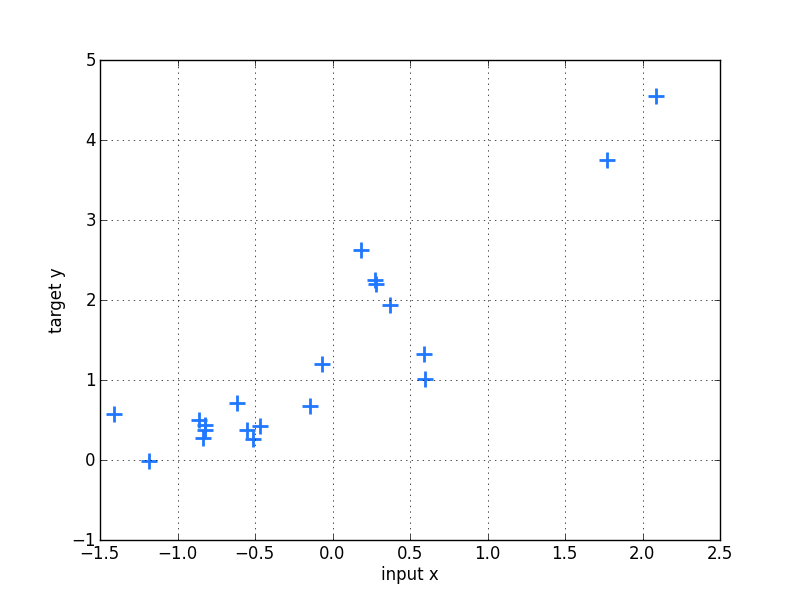
\includegraphics{_images/d1_2.png}}
\end{figure}

You can specify a optimization method different from the default, which is a single run of Rasmussen's minimize. For example, you can choose to rerun the optimization method
several times with different random initializations:

\begin{Verbatim}[commandchars=\\\{\}]
\PYG{n}{model}\PYG{o}{.}\PYG{n}{setOptimizer}\PYG{p}{(}\PYG{l+s}{"}\PYG{l+s}{Minimize}\PYG{l+s}{"}\PYG{p}{,} \PYG{n}{num\PYGZus{}restarts}\PYG{o}{=}\PYG{l+m+mi}{30}\PYG{p}{)}
\end{Verbatim}

The optimized hyperparameters returned by \emph{train()} are then set to be the ones obtained from the run with the best result.
The whole functionality for optimization is introduced in detail in the documentation Optimizers.

Instead of \emph{fit()}, which only fits data using given hyperparameters, \emph{train()} will optimize hyperparamters based on marginal likelihood:

\begin{Verbatim}[commandchars=\\\{\}]
\PYG{n}{model}\PYG{o}{.}\PYG{n}{train}\PYG{p}{(}\PYG{p}{)}
\end{Verbatim}

There are several properties you can get from the model:

\begin{Verbatim}[commandchars=\\\{\}]
\PYG{n}{model}\PYG{o}{.}\PYG{n}{nlZ}                   \PYG{c}{\PYGZsh{} negative log marginal likelihood}
\PYG{n}{model}\PYG{o}{.}\PYG{n}{dnlZ}\PYG{o}{.}\PYG{n}{cov}              \PYG{c}{\PYGZsh{} direvatives of negative log marginal likelihood}
\PYG{n}{model}\PYG{o}{.}\PYG{n}{dnlZ}\PYG{o}{.}\PYG{n}{lik}
\PYG{n}{model}\PYG{o}{.}\PYG{n}{dnlZ}\PYG{o}{.}\PYG{n}{mean}
\PYG{n}{model}\PYG{o}{.}\PYG{n}{posterior}\PYG{o}{.}\PYG{n}{sW}          \PYG{c}{\PYGZsh{} posterior structure}
\PYG{n}{model}\PYG{o}{.}\PYG{n}{posterior}\PYG{o}{.}\PYG{n}{alpha}
\PYG{n}{model}\PYG{o}{.}\PYG{n}{posterior}\PYG{o}{.}\PYG{n}{L}
\PYG{n}{model}\PYG{o}{.}\PYG{n}{covfunc}\PYG{o}{.}\PYG{n}{hyp}
\PYG{n}{model}\PYG{o}{.}\PYG{n}{meanfunc}\PYG{o}{.}\PYG{n}{hyp}
\PYG{n}{model}\PYG{o}{.}\PYG{n}{likfunc}\PYG{o}{.}\PYG{n}{hyp}
\PYG{n}{model}\PYG{o}{.}\PYG{n}{fm}                    \PYG{c}{\PYGZsh{} latent mean}
\PYG{n}{model}\PYG{o}{.}\PYG{n}{fs2}                   \PYG{c}{\PYGZsh{} latent variance}
\PYG{n}{model}\PYG{o}{.}\PYG{n}{ym}                    \PYG{c}{\PYGZsh{} predictive mean}
\PYG{n}{model}\PYG{o}{.}\PYG{n}{ys2}                   \PYG{c}{\PYGZsh{} predictive variance}
\PYG{n}{model}\PYG{o}{.}\PYG{n}{lp}                    \PYG{c}{\PYGZsh{} log predictive probability}
\end{Verbatim}

For example, to get the log marginal likelihood use:

\begin{Verbatim}[commandchars=\\\{\}]
\PYG{k}{print} \PYG{l+s}{'}\PYG{l+s}{Optimized negative log marginal likelihood:}\PYG{l+s}{'}\PYG{p}{,} \PYG{n+nb}{round}\PYG{p}{(}\PYG{n}{model}\PYG{o}{.}\PYG{n}{nlZ}\PYG{p}{,}\PYG{l+m+mi}{3}\PYG{p}{)}
\end{Verbatim}

Prediction on the test data will return five values, which are
output mean (ymu) resp. variance (ys2), latent mean (fmu) resp. variance (fs2), and log predictive probabilities (lp)

\begin{Verbatim}[commandchars=\\\{\}]
\PYG{n}{ym}\PYG{p}{,} \PYG{n}{ys2}\PYG{p}{,} \PYG{n}{fm}\PYG{p}{,} \PYG{n}{fs2}\PYG{p}{,} \PYG{n}{lp} \PYG{o}{=} \PYG{n}{model}\PYG{o}{.}\PYG{n}{predict}\PYG{p}{(}\PYG{n}{z}\PYG{p}{)}
\end{Verbatim}

Plot data. Note that \emph{GPR.plot()} is a toy method only for visualising 1-d data. Here we got a different posterior by using a different prior other than in the default example.

\begin{Verbatim}[commandchars=\\\{\}]
\PYG{n}{model}\PYG{o}{.}\PYG{n}{plot}\PYG{p}{(}\PYG{p}{)}
\end{Verbatim}
\begin{figure}[htbp]
\centering

\scalebox{0.700000}{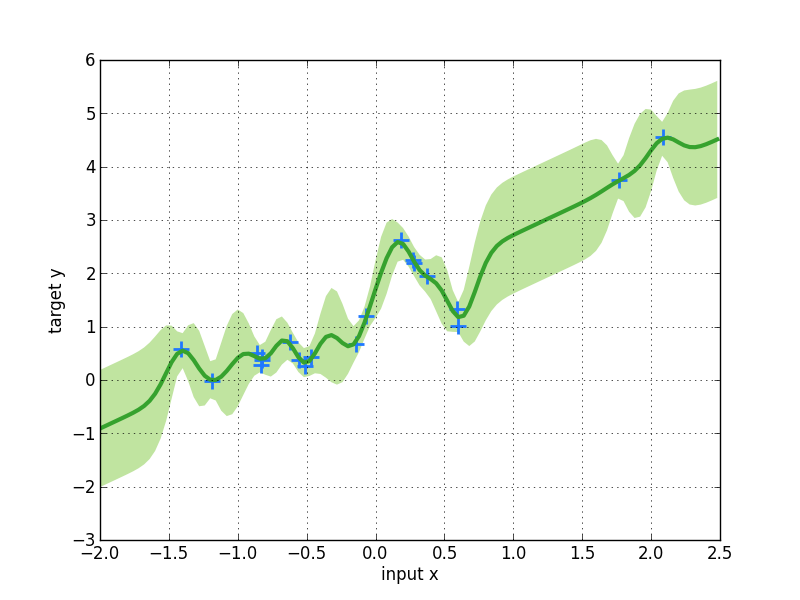
\includegraphics{_images/d1_3.png}}
\end{figure}


\paragraph{A bit more things you can do}
\label{GPR:a-bit-more-things-you-can-do}
\textbf{{[}For all Models{]}} Speed up computation time for prediction if you know posterior in advance. Posterior is passed as an object with three fields (attributes) post.alpha, post.sW and post.L. How to use these vectors to represent the posterior can be best seen from Algorithm 2.1 (page 19) in Chapeter 2 of the \href{http://www.gaussianprocess.org/gpml/chapters/RW2.pdf}{GPML} book by Rasmussen and Williams, 2006.

\begin{Verbatim}[commandchars=\\\{\}]
\PYG{n}{post} \PYG{o}{=} \PYG{n}{myPosterior}\PYG{p}{(}\PYG{p}{)}        \PYG{c}{\PYGZsh{} known in advance}
\PYG{n}{ym}\PYG{p}{,} \PYG{n}{ys2}\PYG{p}{,} \PYG{n}{fm}\PYG{p}{,} \PYG{n}{fs2}\PYG{p}{,} \PYG{n}{lp} \PYG{o}{=} \PYG{n}{model}\PYG{o}{.}\PYG{n}{predict\PYGZus{}with\PYGZus{}posterior}\PYG{p}{(} \PYG{n}{post}\PYG{p}{,}\PYG{n}{z} \PYG{p}{)}
\end{Verbatim}

\textbf{{[}Only for Regression{]}} Specify noise of data (with $\sigma=0.1$ by default):

\begin{Verbatim}[commandchars=\\\{\}]
\PYG{n}{model}\PYG{o}{.}\PYG{n}{setNoise}\PYG{p}{(} \PYG{n}{log\PYGZus{}sigma} \PYG{o}{=} \PYG{n}{np}\PYG{o}{.}\PYG{n}{log}\PYG{p}{(}\PYG{l+m+mf}{0.1}\PYG{p}{)} \PYG{p}{)}
\end{Verbatim}

You do not need to specify the noise parameter if you are optimizing the hyperparamters later anyhow.

All plotting methods have keyword axisvals. You can adjust plotting range if you want. For example:

\begin{Verbatim}[commandchars=\\\{\}]
\PYG{n}{model}\PYG{o}{.}\PYG{n}{plot}\PYG{p}{(}\PYG{n}{axisvals} \PYG{o}{=} \PYG{p}{[}\PYG{o}{-}\PYG{l+m+mf}{1.9}\PYG{p}{,} \PYG{l+m+mf}{1.9}\PYG{p}{,} \PYG{o}{-}\PYG{l+m+mf}{0.9}\PYG{p}{,} \PYG{l+m+mf}{3.9}\PYG{p}{]}\PYG{p}{)}
\end{Verbatim}

Switch to other Inference and Likelihood functions.

\begin{Verbatim}[commandchars=\\\{\}]
\PYG{n}{model}\PYG{o}{.}\PYG{n}{useInference}\PYG{p}{(}\PYG{l+s}{"}\PYG{l+s}{EP}\PYG{l+s}{"}\PYG{p}{)}
\PYG{n}{model}\PYG{o}{.}\PYG{n}{useLikelihood}\PYG{p}{(}\PYG{l+s}{"}\PYG{l+s}{Laplace}\PYG{l+s}{"}\PYG{p}{)}
\end{Verbatim}


\subsubsection{Sparse Regression}
\label{GPR_FITC:sparse-regression}\label{GPR_FITC::doc}
The code shown in this tutorial can be obtained by running \emph{pyGPs/Demo/demo\_GPR\_FITC.py}
This demo is more or less similar to the demo of FITC classification.


\paragraph{First example $\rightarrow$ default inducing points}
\label{GPR_FITC:fitc-classification}\label{GPR_FITC:first-example-default-inducing-points}
First load the same data as in the GPR demo.

\textbf{{[}Theory{]}}
In case the number of training inputs $x$ exceeds a few hundred, approximate inference using Laplace approximation or expectation propagation takes too long. We offer the FITC approximation
based on a low-rank plus diagonal approximation to the exact covariance to deal with these cases. The general idea is to use inducing points
$u$ and to base the computations on cross-covariances between training, test and inducing points only.

Okay, now the model is FITC regression:

\begin{Verbatim}[commandchars=\\\{\}]
\PYG{n}{model} \PYG{o}{=} \PYG{n}{gp}\PYG{o}{.}\PYG{n}{GPR\PYGZus{}FITC}\PYG{p}{(}\PYG{p}{)}
\end{Verbatim}

The difference between the usage of basic $GP$ regression is that we will have to specify inducing points.
In the first example here, we will introduce you how to use the default settings.

The default inducing points are a grid (hypercube for higher dimensions), where each dimension has 5 values in equidistant steps in $[min, max]$,
where $min$ and $max$ are the minimum and maximum values of the input data by default.
In order to specify the dimension of input data, we HAVE TO set data first:

\begin{Verbatim}[commandchars=\\\{\}]
\PYG{n}{model}\PYG{o}{.}\PYG{n}{setData}\PYG{p}{(}\PYG{n}{x}\PYG{p}{,} \PYG{n}{y}\PYG{p}{)}
\end{Verbatim}

The number of inducing points per axis is $5$ per default.

Now, the regular training and prediction routines follow:

\begin{Verbatim}[commandchars=\\\{\}]
\PYG{n}{model}\PYG{o}{.}\PYG{n}{train}\PYG{p}{(}\PYG{p}{)}
\PYG{n}{model}\PYG{o}{.}\PYG{n}{predict}\PYG{p}{(}\PYG{n}{z}\PYG{p}{)}
\PYG{n}{model}\PYG{o}{.}\PYG{n}{plot}\PYG{p}{(}\PYG{p}{)}
\end{Verbatim}
\begin{figure}[htbp]
\centering

\scalebox{0.700000}{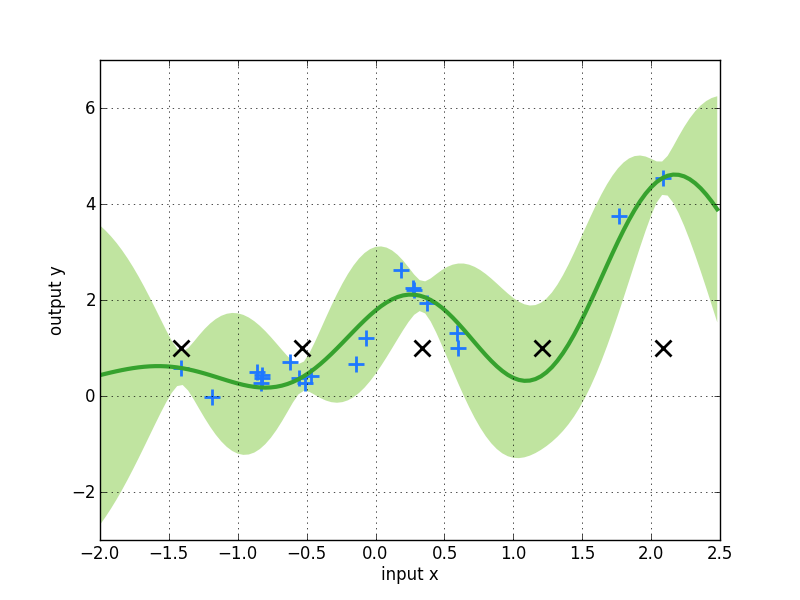
\includegraphics{_images/d3_1.png}}
\end{figure}

The equidistant default inducing points $u$ that are shown in the figure as black x's.

To change the number of inducing points per axis just specify a different value per axis:

\begin{Verbatim}[commandchars=\\\{\}]
\PYG{n}{model}\PYG{o}{.}\PYG{n}{setData}\PYG{p}{(}\PYG{n}{x}\PYG{p}{,} \PYG{n}{y}\PYG{p}{,} \PYG{n}{value\PYGZus{}per\PYGZus{}axis}\PYG{o}{=}\PYG{l+m+mi}{10}\PYG{p}{)}
\end{Verbatim}


\paragraph{Second example $\rightarrow$ user-defined inducing points}
\label{GPR_FITC:second-example-user-defined-inducing-points}
Alternatively, a random subset of the training points can be used as inducing points. Note, that there are plenty of methods to set these inducing points.
So, in the second example let us use a user-defined set of inducing points.

You can pick a set of fixed inducing points by hand:

\begin{Verbatim}[commandchars=\\\{\}]
\PYG{n}{u} \PYG{o}{=} \PYG{n}{np}\PYG{o}{.}\PYG{n}{array}\PYG{p}{(}\PYG{p}{[}\PYG{p}{[}\PYG{o}{-}\PYG{l+m+mi}{1}\PYG{p}{]}\PYG{p}{,} \PYG{p}{[}\PYG{o}{-}\PYG{l+m+mf}{0.8}\PYG{p}{]}\PYG{p}{,} \PYG{p}{[}\PYG{o}{-}\PYG{l+m+mf}{0.5}\PYG{p}{]}\PYG{p}{,} \PYG{p}{[}\PYG{l+m+mf}{0.3}\PYG{p}{]}\PYG{p}{,}\PYG{p}{[}\PYG{l+m+mf}{1.}\PYG{p}{]}\PYG{p}{]}\PYG{p}{)}
\end{Verbatim}

You can also use equidistant inducing points $u$, but without the values on the margin of the grid.(i.e. shrinking the range of values)

\begin{Verbatim}[commandchars=\\\{\}]
\PYG{n}{num\PYGZus{}u} \PYG{o}{=} \PYG{n}{np}\PYG{o}{.}\PYG{n}{fix}\PYG{p}{(}\PYG{n}{x}\PYG{o}{.}\PYG{n}{shape}\PYG{p}{[}\PYG{l+m+mi}{0}\PYG{p}{]}\PYG{o}{/}\PYG{l+m+mi}{2}\PYG{p}{)}
\PYG{n}{u} \PYG{o}{=} \PYG{n}{np}\PYG{o}{.}\PYG{n}{linspace}\PYG{p}{(}\PYG{o}{-}\PYG{l+m+mf}{1.3}\PYG{p}{,}\PYG{l+m+mf}{1.3}\PYG{p}{,}\PYG{n}{num\PYGZus{}u}\PYG{p}{)}\PYG{o}{.}\PYG{n}{T}
\PYG{n}{u} \PYG{o}{=} \PYG{n}{np}\PYG{o}{.}\PYG{n}{reshape}\PYG{p}{(}\PYG{n}{u}\PYG{p}{,}\PYG{p}{(}\PYG{n}{num\PYGZus{}u}\PYG{p}{,}\PYG{l+m+mi}{1}\PYG{p}{)}\PYG{p}{)}
\end{Verbatim}

Then pass $u$ when specifying prior.

\begin{Verbatim}[commandchars=\\\{\}]
\PYG{n}{m} \PYG{o}{=} \PYG{n}{mean}\PYG{o}{.}\PYG{n}{Zero}\PYG{p}{(}\PYG{p}{)}
\PYG{n}{k} \PYG{o}{=} \PYG{n}{cov}\PYG{o}{.}\PYG{n}{RBFard}\PYG{p}{(}\PYG{n}{log\PYGZus{}ell\PYGZus{}list}\PYG{o}{=}\PYG{p}{[}\PYG{l+m+mf}{0.05}\PYG{p}{,}\PYG{l+m+mf}{0.17}\PYG{p}{]}\PYG{p}{,} \PYG{n}{log\PYGZus{}sigma}\PYG{o}{=}\PYG{l+m+mf}{1.}\PYG{p}{)}
\PYG{n}{model}\PYG{o}{.}\PYG{n}{setPrior}\PYG{p}{(}\PYG{n}{mean}\PYG{o}{=}\PYG{n}{m}\PYG{p}{,} \PYG{n}{kernel}\PYG{o}{=}\PYG{n}{k}\PYG{p}{,} \PYG{n}{inducing\PYGZus{}points}\PYG{o}{=}\PYG{n}{u}\PYG{p}{)}
\end{Verbatim}

The left figure below shows the result of fixed inducing points, and the right figure shows the result for equidistant $u$.

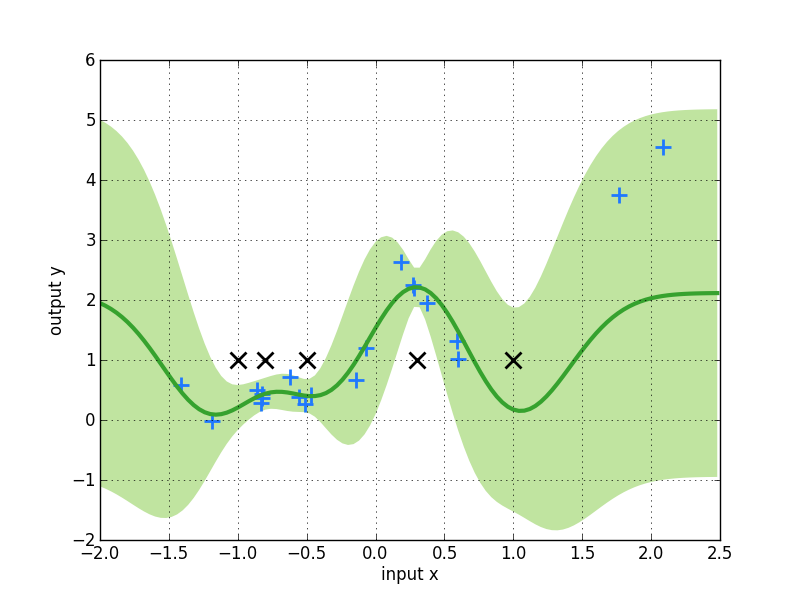
\includegraphics[width=0.450\linewidth]{_images/d3_2.png}

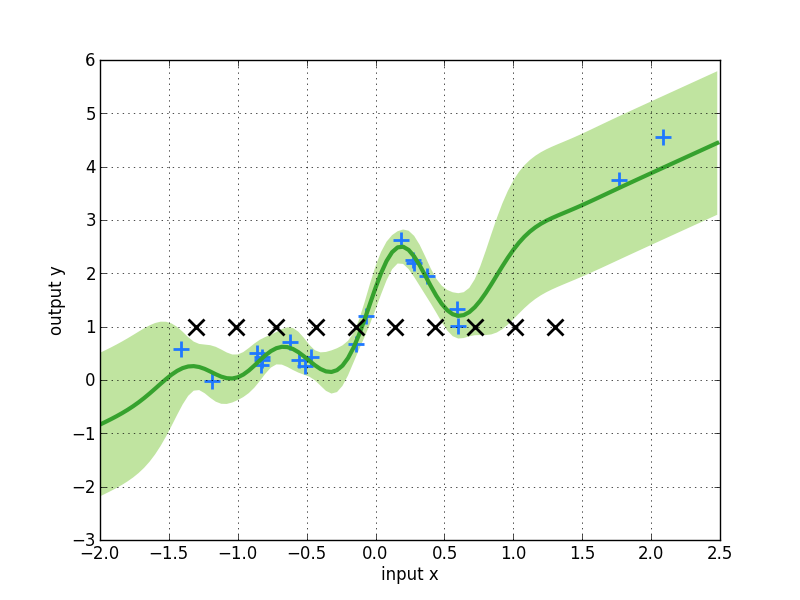
\includegraphics[width=0.450\linewidth]{_images/d3_3.png}

\textbf{{[}Theory{]}}
Note that the predictive variance is
overestimated outside the support of the inducing inputs. In a multivariate example where densely sampled inducing inputs are infeasible, one can
also try to simply use a random subset of the training points.


\paragraph{A bit more things you can do}
\label{GPR_FITC:a-bit-more-things-you-can-do}
Switch to other Inference and Likelihood functions.

\begin{Verbatim}[commandchars=\\\{\}]
\PYG{n}{model}\PYG{o}{.}\PYG{n}{useInference}\PYG{p}{(}\PYG{l+s}{"}\PYG{l+s}{EP}\PYG{l+s}{"}\PYG{p}{)}
\PYG{n}{model}\PYG{o}{.}\PYG{n}{useLikelihood}\PYG{p}{(}\PYG{l+s}{"}\PYG{l+s}{Laplace}\PYG{l+s}{"}\PYG{p}{)}
\end{Verbatim}

Classification


\subsubsection{Basic Classification}
\label{GPC:basic-classification}\label{GPC::doc}
The demo shown in this tutorial can be obtained by running \emph{pyGPs/Demo/demo\_GPC.py}.


\paragraph{Load data}
\label{GPC:load-data}
First, we import the data:

\begin{Verbatim}[commandchars=\\\{\}]
\PYG{c}{\PYGZsh{} GPC target class are +1 and -1}
\PYG{n}{demoData} \PYG{o}{=} \PYG{n}{np}\PYG{o}{.}\PYG{n}{load}\PYG{p}{(}\PYG{l+s}{'}\PYG{l+s}{data\PYGZus{}for\PYGZus{}demo/classification\PYGZus{}data.npz}\PYG{l+s}{'}\PYG{p}{)}
\PYG{n}{x} \PYG{o}{=} \PYG{n}{demoData}\PYG{p}{[}\PYG{l+s}{'}\PYG{l+s}{x}\PYG{l+s}{'}\PYG{p}{]}            \PYG{c}{\PYGZsh{} training data}
\PYG{n}{y} \PYG{o}{=} \PYG{n}{demoData}\PYG{p}{[}\PYG{l+s}{'}\PYG{l+s}{y}\PYG{l+s}{'}\PYG{p}{]}            \PYG{c}{\PYGZsh{} training target}
\PYG{n}{z} \PYG{o}{=} \PYG{n}{demoData}\PYG{p}{[}\PYG{l+s}{'}\PYG{l+s}{xstar}\PYG{l+s}{'}\PYG{p}{]}        \PYG{c}{\PYGZsh{} test data}
\end{Verbatim}

The $120$ data points were generated from two Gaussians with different means and covariances. One Gaussian is isotropic and contains
$2/3$ of the data (blue), the other is highly correlated and contains $1/3$ of the points (red).
Note, that the labels for the targets are specified to be $\pm 1$ (and not $0/1$).

In the plot, we superimpose the data points with the posterior equi-probability contour lines for the probability of the second class
given complete information about the generating mechanism.
\begin{figure}[htbp]
\centering

\scalebox{0.700000}{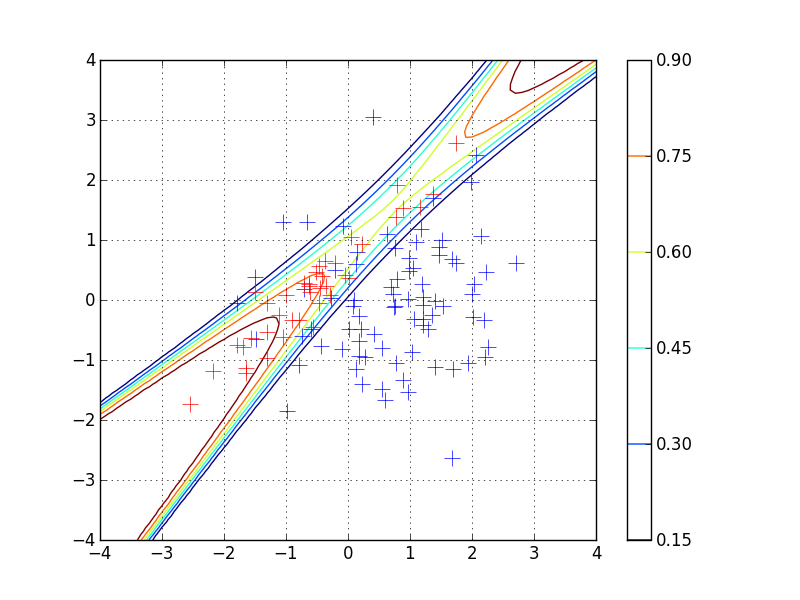
\includegraphics{_images/d2_1.png}}
\end{figure}


\paragraph{First example $\rightarrow$ state default values}
\label{GPC:first-example-state-default-values}
Again, lets see the simplest use of gp classification at first

\begin{Verbatim}[commandchars=\\\{\}]
\PYG{n}{model} \PYG{o}{=} \PYG{n}{gp}\PYG{o}{.}\PYG{n}{GPC}\PYG{p}{(}\PYG{p}{)}             \PYG{c}{\PYGZsh{} binary classification (default inference method: EP)}
\PYG{n}{model}\PYG{o}{.}\PYG{n}{fit}\PYG{p}{(}\PYG{n}{x}\PYG{p}{,} \PYG{n}{y}\PYG{p}{)}              \PYG{c}{\PYGZsh{} fit default model (mean zero \& rbf kernel) with data}
\PYG{n}{model}\PYG{o}{.}\PYG{n}{train}\PYG{p}{(}\PYG{n}{x}\PYG{p}{,} \PYG{n}{y}\PYG{p}{)}            \PYG{c}{\PYGZsh{} optimize hyperparamters (default optimizer: single run minimize)}
\PYG{n}{model}\PYG{o}{.}\PYG{n}{predict}\PYG{p}{(}\PYG{n}{z}\PYG{p}{)}             \PYG{c}{\PYGZsh{} predict test cases}
\end{Verbatim}

Note, that inference is done via expectation propagation (EP) approximation by deault. How to set inference to Laplace approximation, see {\hyperref[GPC:more-on-gpc]{\emph{A bit more things you can do}}}.


\paragraph{Second example $\rightarrow$ GP classification}
\label{GPC:second-example-gp-classification}
So we first state the model to be $GP$ classification now:

\begin{Verbatim}[commandchars=\\\{\}]
\PYG{n}{model} \PYG{o}{=} \PYG{n}{gp}\PYG{o}{.}\PYG{n}{GPC}\PYG{p}{(}\PYG{p}{)}
\end{Verbatim}

The rest is similar to GPR:

\begin{Verbatim}[commandchars=\\\{\}]
\PYG{n}{k} \PYG{o}{=} \PYG{n}{cov}\PYG{o}{.}\PYG{n}{RBFard}\PYG{p}{(}\PYG{n}{log\PYGZus{}ell\PYGZus{}list}\PYG{o}{=}\PYG{p}{[}\PYG{l+m+mf}{0.05}\PYG{p}{,}\PYG{l+m+mf}{0.17}\PYG{p}{]}\PYG{p}{,} \PYG{n}{log\PYGZus{}sigma}\PYG{o}{=}\PYG{l+m+mf}{1.}\PYG{p}{)}
\PYG{n}{model}\PYG{o}{.}\PYG{n}{setPrior}\PYG{p}{(}\PYG{n}{kernel}\PYG{o}{=}\PYG{n}{k}\PYG{p}{)}

\PYG{n}{model}\PYG{o}{.}\PYG{n}{setData}\PYG{p}{(}\PYG{n}{x}\PYG{p}{,} \PYG{n}{y}\PYG{p}{)}
\PYG{n}{model}\PYG{o}{.}\PYG{n}{plotData\PYGZus{}2d}\PYG{p}{(}\PYG{n}{x1}\PYG{p}{,}\PYG{n}{x2}\PYG{p}{,}\PYG{n}{t1}\PYG{p}{,}\PYG{n}{t2}\PYG{p}{,}\PYG{n}{p1}\PYG{p}{,}\PYG{n}{p2}\PYG{p}{)}

\PYG{n}{model}\PYG{o}{.}\PYG{n}{fit}\PYG{p}{(}\PYG{p}{)}
\PYG{n}{model}\PYG{o}{.}\PYG{n}{train}\PYG{p}{(}\PYG{p}{)}
\PYG{n}{model}\PYG{o}{.}\PYG{n}{predict}\PYG{p}{(}\PYG{n}{z}\PYG{p}{,} \PYG{n}{ys}\PYG{o}{=}\PYG{n}{np}\PYG{o}{.}\PYG{n}{ones}\PYG{p}{(}\PYG{p}{(}\PYG{n}{z}\PYG{o}{.}\PYG{n}{shape}\PYG{p}{[}\PYG{l+m+mi}{0}\PYG{p}{]}\PYG{p}{,}\PYG{l+m+mi}{1}\PYG{p}{)}\PYG{p}{)}\PYG{p}{)}
\end{Verbatim}

\textbf{{[}Theory{]}}
In this example, we used an RBF kernel (squared exponential covariance function) with automatic relevance determination (ARD). This covariance function has one
characteristic length-scale parameter for each dimension of the input space (here $2$ in total), and a signal magnitude parameter, resulting in
a total of $3$ hyperparameters. ARD with separate length-scales for each input dimension is a very powerful tool to learn which
inputs are important for the predictions: if length-scales are short, input dimensions are very important, and when they grow very large
(compared to the spread of the data), the corresponding input dimensions will be mostly ignored.

Note, \emph{GPC.plot()} is a toy method for 2-d data:

\begin{Verbatim}[commandchars=\\\{\}]
\PYG{n}{model}\PYG{o}{.}\PYG{n}{plot}\PYG{p}{(}\PYG{n}{x1}\PYG{p}{,}\PYG{n}{x2}\PYG{p}{,}\PYG{n}{t1}\PYG{p}{,}\PYG{n}{t2}\PYG{p}{)}
\end{Verbatim}

The contour plot for the predictive distribution is shown below. Note, that the predictive
probability is fairly close to the probabilities of the generating process in regions of high data density. Note also, that as you move
away from the data, the probability approaches $1/3$, the overall class probability.
\begin{figure}[htbp]
\centering

\scalebox{0.700000}{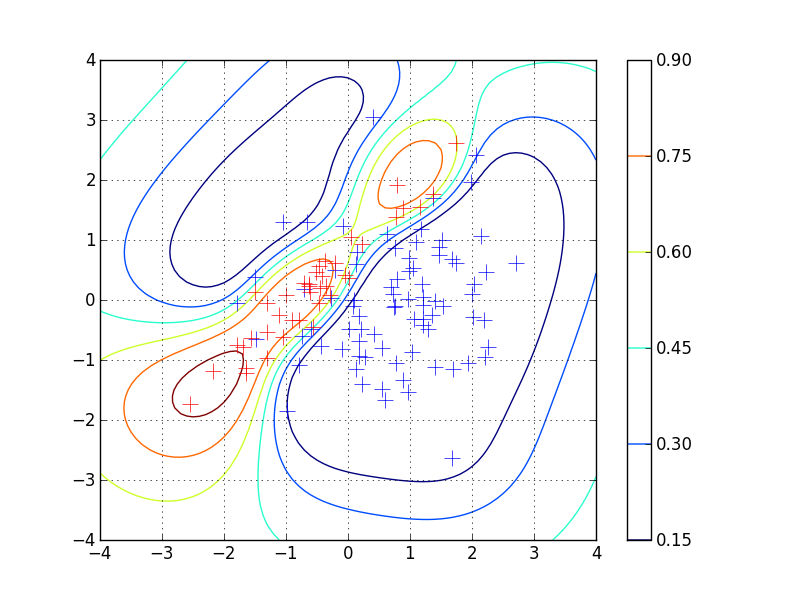
\includegraphics{_images/d2_2.png}}
\end{figure}

Examining the two ARD characteristic length-scale parameters after learning, you will find that they are fairly similar, reflecting the fact
that for this data set, both input dimensions are important.


\paragraph{A bit more things you can do}
\label{GPC:a-bit-more-things-you-can-do}\label{GPC:more-on-gpc}
GPC uses expectation propagation (EP)  inference and Error function likelihood by default, you can explictly change to other methods:

\begin{Verbatim}[commandchars=\\\{\}]
\PYG{n}{model}\PYG{o}{.}\PYG{n}{useInference}\PYG{p}{(}\PYG{l+s}{"}\PYG{l+s}{Laplace}\PYG{l+s}{"}\PYG{p}{)}
\end{Verbatim}


\subsubsection{Sparse Classification}
\label{GPC_FITC:sparse-classification}\label{GPC_FITC::doc}
The demo in this tutorial can be obtained by running \emph{pyGPs/Demo/demo\_GPC\_FITC.py}.
This demo is more or less a repetition of the demo of FITC regression.


\paragraph{First example $\rightarrow$ default inducing points}
\label{GPC_FITC:fitc-regression}\label{GPC_FITC:first-example-default-inducing-points}
First load the same data as in the GPC demo.

\textbf{{[}Theory{]}}
In case the number of training inputs $x$ exceeds a few hundred, approximate inference using Laplacian Approximation or Expectation Propagation takes too long. As in regression, we offer the FITC approximation
based on a low-rank plus diagonal approximation to the exact covariance to deal with these cases. The general idea is to use inducing points
$u$ and to base the computations on cross-covariances between training, test and inducing points only.

Okay, now the model is FITC classificiation:

\begin{Verbatim}[commandchars=\\\{\}]
\PYG{n}{model} \PYG{o}{=} \PYG{n}{gp}\PYG{o}{.}\PYG{n}{GPC\PYGZus{}FITC}\PYG{p}{(}\PYG{p}{)}
\end{Verbatim}

The difference between the usage of basic $GP$ is that we will have to specify inducing points.
In our first example, we will introduce how to perform sparse GPC with the default settings.

The default inducing points form a grid (hypercube in higher dimension), where each dimension has $5$ values in equidistant steps in $[min, max]$,
where $min$ and $max$ are the minimum and maximum values of the input data by default.
In order to specify the dimension of input data, we HAVE TO set data first:

\begin{Verbatim}[commandchars=\\\{\}]
\PYG{n}{model}\PYG{o}{.}\PYG{n}{setData}\PYG{p}{(}\PYG{n}{x}\PYG{p}{,} \PYG{n}{y}\PYG{p}{)}
\end{Verbatim}

The number of inducing points per axis is $5$ per default. How to change this, see {\hyperref[GPC_FITC:more-on-gpc-fitc]{\emph{A bit more things you can do}}}.

Then, the regular process follows:

\begin{Verbatim}[commandchars=\\\{\}]
\PYG{n}{model}\PYG{o}{.}\PYG{n}{train}\PYG{p}{(}\PYG{p}{)}
\PYG{n}{model}\PYG{o}{.}\PYG{n}{predict}\PYG{p}{(}\PYG{n}{z}\PYG{p}{,} \PYG{n}{ys}\PYG{o}{=}\PYG{n}{np}\PYG{o}{.}\PYG{n}{ones}\PYG{p}{(}\PYG{p}{(}\PYG{n}{z}\PYG{o}{.}\PYG{n}{shape}\PYG{p}{[}\PYG{l+m+mi}{0}\PYG{p}{]}\PYG{p}{,}\PYG{l+m+mi}{1}\PYG{p}{)}\PYG{p}{)}\PYG{p}{)}
\PYG{n}{model}\PYG{o}{.}\PYG{n}{plot}\PYG{p}{(}\PYG{n}{x1}\PYG{p}{,}\PYG{n}{x2}\PYG{p}{,}\PYG{n}{t1}\PYG{p}{,}\PYG{n}{t2}\PYG{p}{)}
\end{Verbatim}
\begin{figure}[htbp]
\centering

\scalebox{0.700000}{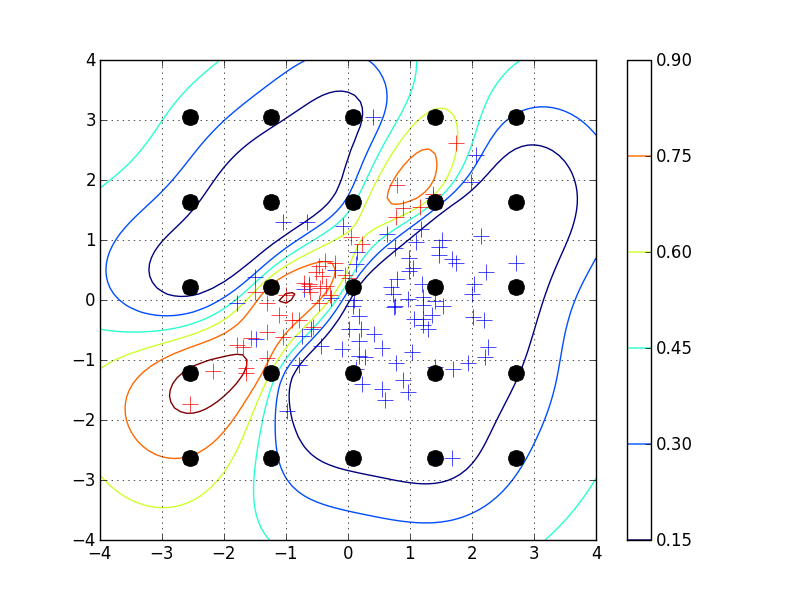
\includegraphics{_images/d4_1.png}}
\end{figure}

The equispaced default inducing points $u$ are shown as black circles in the plot.


\paragraph{Second example $\rightarrow$ user-defined inducing points}
\label{GPC_FITC:second-example-user-defined-inducing-points}
Alternatively, a random subset of the training points can be used as inducing points. Note, that there are various different ways of how to set the inducing points.
So, in the second example let us use a user-defined set of inducing points:

\begin{Verbatim}[commandchars=\\\{\}]
\PYG{n}{u1}\PYG{p}{,}\PYG{n}{u2} \PYG{o}{=} \PYG{n}{np}\PYG{o}{.}\PYG{n}{meshgrid}\PYG{p}{(}\PYG{n}{np}\PYG{o}{.}\PYG{n}{linspace}\PYG{p}{(}\PYG{o}{-}\PYG{l+m+mi}{2}\PYG{p}{,}\PYG{l+m+mi}{2}\PYG{p}{,}\PYG{l+m+mi}{5}\PYG{p}{)}\PYG{p}{,}\PYG{n}{np}\PYG{o}{.}\PYG{n}{linspace}\PYG{p}{(}\PYG{o}{-}\PYG{l+m+mi}{2}\PYG{p}{,}\PYG{l+m+mi}{2}\PYG{p}{,}\PYG{l+m+mi}{5}\PYG{p}{)}\PYG{p}{)}
\PYG{n}{u} \PYG{o}{=} \PYG{n}{np}\PYG{o}{.}\PYG{n}{array}\PYG{p}{(}\PYG{n+nb}{zip}\PYG{p}{(}\PYG{n}{np}\PYG{o}{.}\PYG{n}{reshape}\PYG{p}{(}\PYG{n}{u2}\PYG{p}{,}\PYG{p}{(}\PYG{n}{np}\PYG{o}{.}\PYG{n}{prod}\PYG{p}{(}\PYG{n}{u2}\PYG{o}{.}\PYG{n}{shape}\PYG{p}{)}\PYG{p}{,}\PYG{p}{)}\PYG{p}{)}\PYG{p}{,}\PYG{n}{np}\PYG{o}{.}\PYG{n}{reshape}\PYG{p}{(}\PYG{n}{u1}\PYG{p}{,}\PYG{p}{(}\PYG{n}{np}\PYG{o}{.}\PYG{n}{prod}\PYG{p}{(}\PYG{n}{u1}\PYG{o}{.}\PYG{n}{shape}\PYG{p}{)}\PYG{p}{,}\PYG{p}{)}\PYG{p}{)}\PYG{p}{)}\PYG{p}{)}
\end{Verbatim}

Here, we also use a grid euqually spaced, but without the values on the margin of the grid.(i.e. shrinking the grid) Then, we can just pass $u$ when specifying prior:

\begin{Verbatim}[commandchars=\\\{\}]
\PYG{n}{m} \PYG{o}{=} \PYG{n}{mean}\PYG{o}{.}\PYG{n}{Zero}\PYG{p}{(}\PYG{p}{)}
\PYG{n}{k} \PYG{o}{=} \PYG{n}{cov}\PYG{o}{.}\PYG{n}{RBFard}\PYG{p}{(}\PYG{n}{log\PYGZus{}ell\PYGZus{}list}\PYG{o}{=}\PYG{p}{[}\PYG{l+m+mf}{0.05}\PYG{p}{,}\PYG{l+m+mf}{0.17}\PYG{p}{]}\PYG{p}{,} \PYG{n}{log\PYGZus{}sigma}\PYG{o}{=}\PYG{l+m+mf}{1.}\PYG{p}{)}
\PYG{n}{model}\PYG{o}{.}\PYG{n}{setPrior}\PYG{p}{(}\PYG{n}{mean}\PYG{o}{=}\PYG{n}{m}\PYG{p}{,} \PYG{n}{kernel}\PYG{o}{=}\PYG{n}{k}\PYG{p}{,} \PYG{n}{inducing\PYGZus{}points}\PYG{o}{=}\PYG{n}{u}\PYG{p}{)}
\end{Verbatim}

The prediction results for this  set of inducing points are shown below:
\begin{figure}[htbp]
\centering

\scalebox{0.700000}{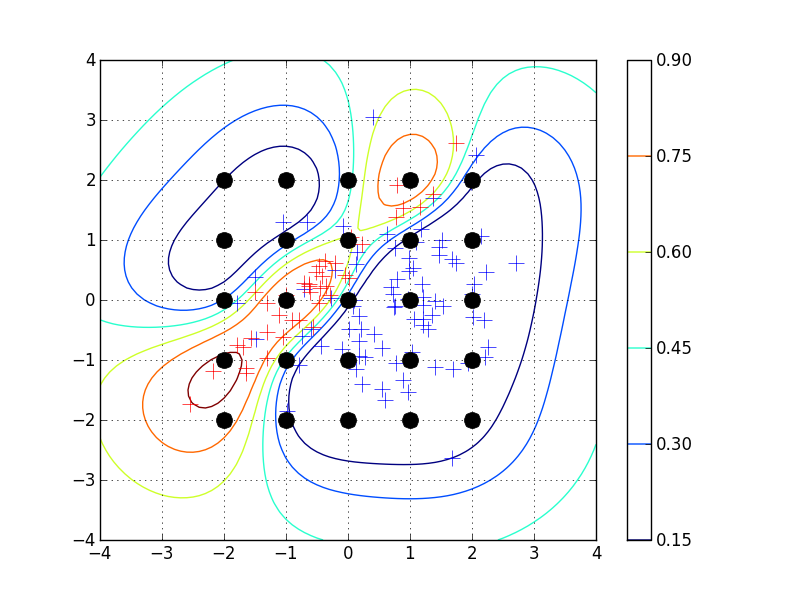
\includegraphics{_images/d4_2.png}}
\end{figure}


\paragraph{A bit more things you can do}
\label{GPC_FITC:more-on-gpc-fitc}\label{GPC_FITC:a-bit-more-things-you-can-do}
As in standard GPC, it is possible to use other inference/likelihood in the FITC method:

\begin{Verbatim}[commandchars=\\\{\}]
\PYG{n}{model}\PYG{o}{.}\PYG{n}{useInference}\PYG{p}{(}\PYG{l+s}{"}\PYG{l+s}{Laplace}\PYG{l+s}{"}\PYG{p}{)}
\end{Verbatim}

Change the number of inducing points per axis:

\begin{Verbatim}[commandchars=\\\{\}]
\PYG{n}{model}\PYG{o}{.}\PYG{n}{setData}\PYG{p}{(}\PYG{n}{x}\PYG{p}{,} \PYG{n}{y}\PYG{p}{,} \PYG{n}{value\PYGZus{}per\PYGZus{}axis}\PYG{o}{=}\PYG{l+m+mi}{10}\PYG{p}{)}
\end{Verbatim}


\subsubsection{Multi-class Classification}
\label{GPMC::doc}\label{GPMC:multi-class-classification}
GPMC is NOT based on multi-class Laplace approximation.
It works as a one vs. one classification wrapper.
In other words, GPMC trains a GPC model for each pair of two classes,
and uses a majority voting scheme over all results to determine the final class.
The method only returns the predictive class with highest rating;
no other values (such as variance) are returned.

Lets see a practical example to classify the 10 (0,1,2,...9) hand-written digits
in the USPS digits dataset.


\paragraph{Load data}
\label{GPMC:load-data}
The USPS digits data were gathered at the Center of Excellence in Document Analysis and Recognition (CEDAR) at SUNY Buffalo, as part of a project sponsored by the US Postal Service. The dataset is described in \footnote{
A Database for Handwritten Text Recognition Research, J. J. Hull, IEEE PAMI 16(5) 550-554, 1994.
}.

\begin{Verbatim}[commandchars=\\\{\}]
\PYG{n}{data} \PYG{o}{=} \PYG{n}{loadmat}\PYG{p}{(}\PYG{l+s}{'}\PYG{l+s}{data\PYGZus{}for\PYGZus{}demo/usps\PYGZus{}resampled.mat}\PYG{l+s}{'}\PYG{p}{)}
\PYG{n}{x} \PYG{o}{=} \PYG{n}{data}\PYG{p}{[}\PYG{l+s}{'}\PYG{l+s}{train\PYGZus{}patterns}\PYG{l+s}{'}\PYG{p}{]}\PYG{o}{.}\PYG{n}{T}   \PYG{c}{\PYGZsh{} train patterns}
\PYG{n}{y} \PYG{o}{=} \PYG{n}{data}\PYG{p}{[}\PYG{l+s}{'}\PYG{l+s}{train\PYGZus{}labels}\PYG{l+s}{'}\PYG{p}{]}\PYG{o}{.}\PYG{n}{T}     \PYG{c}{\PYGZsh{} train labels}
\PYG{n}{xs} \PYG{o}{=} \PYG{n}{data}\PYG{p}{[}\PYG{l+s}{'}\PYG{l+s}{test\PYGZus{}patterns}\PYG{l+s}{'}\PYG{p}{]}\PYG{o}{.}\PYG{n}{T}   \PYG{c}{\PYGZsh{} test patterns}
\PYG{n}{ys} \PYG{o}{=} \PYG{n}{data}\PYG{p}{[}\PYG{l+s}{'}\PYG{l+s}{test\PYGZus{}labels}\PYG{l+s}{'}\PYG{p}{]}\PYG{o}{.}\PYG{n}{T}     \PYG{c}{\PYGZsh{} test labels}
\end{Verbatim}

To be used in GPMC, labels should start from 0 to k (k = number of classes).


\paragraph{GPMC example}
\label{GPMC:gpmc-example}
State model with 10-class classification problem:

\begin{Verbatim}[commandchars=\\\{\}]
\PYG{n}{model} \PYG{o}{=} \PYG{n}{gp}\PYG{o}{.}\PYG{n}{GPMC}\PYG{p}{(}\PYG{l+m+mi}{10}\PYG{p}{)}
\end{Verbatim}

Pass data to model:

\begin{Verbatim}[commandchars=\\\{\}]
\PYG{n}{model}\PYG{o}{.}\PYG{n}{setData}\PYG{p}{(}\PYG{n}{x}\PYG{p}{,}\PYG{n}{y}\PYG{p}{)}
\end{Verbatim}

Train default GPC model for each binary classification problem,
and decide label for test patterns of hand-writen digits.
The return value \emph{predictive\_vote{[}i,j{]}} is the probability of being class \emph{j} for test pattern \emph{i}.

\begin{Verbatim}[commandchars=\\\{\}]
\PYG{n}{predictive\PYGZus{}vote} \PYG{o}{=} \PYG{n}{model}\PYG{o}{.}\PYG{n}{trainAndPredict}\PYG{p}{(}\PYG{n}{xs}\PYG{p}{)}
\PYG{n}{predictive\PYGZus{}class} \PYG{o}{=} \PYG{n}{np}\PYG{o}{.}\PYG{n}{argmax}\PYG{p}{(}\PYG{n}{predictive\PYGZus{}vote}\PYG{p}{,} \PYG{n}{axis}\PYG{o}{=}\PYG{l+m+mi}{1}\PYG{p}{)}
\end{Verbatim}

Just like we did for GP classification,
you can use specific settings (other than default) for all binary classificiation problem for example by:

\begin{Verbatim}[commandchars=\\\{\}]
\PYG{n}{m} \PYG{o}{=} \PYG{n}{mean}\PYG{o}{.}\PYG{n}{Zero}\PYG{p}{(}\PYG{p}{)}
\PYG{n}{k} \PYG{o}{=} \PYG{n}{cov}\PYG{o}{.}\PYG{n}{RBF}\PYG{p}{(}\PYG{p}{)}
\PYG{n}{model}\PYG{o}{.}\PYG{n}{setPrior}\PYG{p}{(}\PYG{n}{mean}\PYG{o}{=}\PYG{n}{m}\PYG{p}{,}\PYG{n}{kernel}\PYG{o}{=}\PYG{n}{k}\PYG{p}{)}
\PYG{n}{model}\PYG{o}{.}\PYG{n}{useInference}\PYG{p}{(}\PYG{l+s}{"}\PYG{l+s}{Laplace}\PYG{l+s}{"}\PYG{p}{)}
\end{Verbatim}

For more information on how to use non-default settings see demo\_GPC and demo\_GPR.

Beside \emph{trainAndPredict(xs)},
there is also an option to perform prediction without hyperparameter optimization:

\begin{Verbatim}[commandchars=\\\{\}]
\PYG{n}{model}\PYG{o}{.}\PYG{n}{fitAndPredict}\PYG{p}{(}\PYG{n}{xs}\PYG{p}{)}
\end{Verbatim}

Some examples for real-world data


\subsubsection{K-fold Cross-Validation}
\label{CV:k-fold-cross-validation}\label{CV::doc}
In this demo, we'll show you the typical process of using GP for machine learning from loading data, preprocessing, training,  predicting to validation and evaluation.


\paragraph{Load data}
\label{CV:load-data}
We use the ionosphere dataset \footnote{
Sigillito, V. G., Wing, S. P., Hutton, L. V., \& Baker, K. B. (1989). Classification of radar returns from the ionosphere using neural networks. Johns Hopkins APL Technical Digest, 10, 262-266.
} from Johns Hopkins University Ionosphere database.
It is available in UCI machine learning repository.
Then we need to do some data cleaning. Here we deal with label in ionosphere data, change ``b'' to''-1'', and ``g'' to ``+1''. These preprocessing implementation are availabe in the source code.


\paragraph{Cross Validation}
\label{CV:cross-validation}
Now, lets focus on the use of cross-validation.

\begin{Verbatim}[commandchars=\\\{\}]
\PYG{n}{K} \PYG{o}{=} \PYG{l+m+mi}{10}             \PYG{c}{\PYGZsh{} number of folds}
\PYG{k}{for} \PYG{n}{x\PYGZus{}train}\PYG{p}{,} \PYG{n}{x\PYGZus{}test}\PYG{p}{,} \PYG{n}{y\PYGZus{}train}\PYG{p}{,} \PYG{n}{y\PYGZus{}test} \PYG{o+ow}{in} \PYG{n}{valid}\PYG{o}{.}\PYG{n}{k\PYGZus{}fold\PYGZus{}validation}\PYG{p}{(}\PYG{n}{x}\PYG{p}{,} \PYG{n}{y}\PYG{p}{,} \PYG{n}{K}\PYG{p}{)}\PYG{p}{:}
    \PYG{c}{\PYGZsh{} This is a binary classification problem}
    \PYG{n}{model} \PYG{o}{=} \PYG{n}{gp}\PYG{o}{.}\PYG{n}{GPC}\PYG{p}{(}\PYG{p}{)}
    \PYG{c}{\PYGZsh{} Since no prior knowldege, leave everything default}
    \PYG{n}{model}\PYG{o}{.}\PYG{n}{train}\PYG{p}{(}\PYG{n}{x\PYGZus{}train}\PYG{p}{,} \PYG{n}{y\PYGZus{}train}\PYG{p}{)}
    \PYG{c}{\PYGZsh{} Predition}
    \PYG{n}{ymu}\PYG{p}{,} \PYG{n}{ys2}\PYG{p}{,} \PYG{n}{fmu}\PYG{p}{,} \PYG{n}{fs2}\PYG{p}{,} \PYG{n}{lp} \PYG{o}{=} \PYG{n}{model}\PYG{o}{.}\PYG{n}{predict}\PYG{p}{(}\PYG{n}{x\PYGZus{}test}\PYG{p}{,} \PYG{n}{ys}\PYG{o}{=}\PYG{n}{y\PYGZus{}test}\PYG{p}{)}
    \PYG{c}{\PYGZsh{} ymu for classification is a continuous value over -1 to +1}
    \PYG{c}{\PYGZsh{} If you want predicting result to either one of the classes, take a sign of ymu.}
    \PYG{n}{ymu\PYGZus{}class} \PYG{o}{=} \PYG{n}{np}\PYG{o}{.}\PYG{n}{sign}\PYG{p}{(}\PYG{n}{ymu}\PYG{p}{)}
    \PYG{c}{\PYGZsh{} Evluation}
    \PYG{n}{acc} \PYG{o}{=} \PYG{n}{valid}\PYG{o}{.}\PYG{n}{ACC}\PYG{p}{(}\PYG{n}{ymu\PYGZus{}class}\PYG{p}{,} \PYG{n}{y\PYGZus{}test}\PYG{p}{)}       \PYG{c}{\PYGZsh{} accuracy}
    \PYG{n}{rmse} \PYG{o}{=} \PYG{n}{valid}\PYG{o}{.}\PYG{n}{RMSE}\PYG{p}{(}\PYG{n}{ymu\PYGZus{}class}\PYG{p}{,} \PYG{n}{y\PYGZus{}test}\PYG{p}{)}     \PYG{c}{\PYGZsh{} root-mean-square error}
\end{Verbatim}


\paragraph{Evaluation measures}
\label{CV:evaluation-measures}\begin{description}
\item[{We implemented some classical evaluation measures.}] \leavevmode\begin{itemize}
\item {} 
RMSE - root mean squared error

\item {} 
ACC - classification/regression accuracy

\item {} 
Prec - classification precision for class +1

\item {} 
Recall - classification recall for class +1

\item {} 
NLPD - negative log predictive density in transformed observation space

\end{itemize}

\end{description}


\subsubsection{Regression on Mauna Loa data}
\label{demoMaunaLoa:regression-on-mauna-loa-data}\label{demoMaunaLoa::doc}
This example does regression on the Hawaiian Mauna Loa data (example taken from chapter $5$ of the \href{http://www.gaussianprocess.org/gpml/chapters/RW5.pdf}{GPML} book by Rasmussen and Williams, 2006)

We will use a modelling problem concerning the concentration of $CO_2$
in the atmosphere to illustrate how the marginal likelihood can be used to set multiple
hyperparameters in hierarchical Gaussian process models. A complex covariance function
is derived by combining several different kinds of simple covariance
functions, and the resulting model provides an excellent fit to the data as well
as insight into its properties by interpretation of the adapted hyperparameters. Although the data is
one-dimensional, and therefore easy to visualize, a
total of $11$ hyperparameters are used, which in practice rules out the use of
cross-validation for setting parameters, except for the gradient-based LOO-CV procedure.

The data \footnote{
Keeling, C. D. and Whorf, T. P. (2004). Atmospheric $CO_2$ Records from Sites in the SIO Air Sampling Network. In Trends: A Compendium of Data on Global Change. Carbon Dioxide Information Analysis Center, Oak Ridge National Laboratory, Oak Ridge, Tenn., U.S.A.
} consists of monthly average atmospheric $CO_2$
concentrations (in parts per million by volume (ppmv)) derived from \emph{in-situ}
air samples collected at the Mauna Loa Observatory, Hawaii, between $1958$ and
$2003$ (with some missing values) \href{http://cdiac.esd.ornl.gov/ftp/trends/co2/maunaloa.co2}{{[}2{]}}.
\begin{figure}[htbp]
\centering

\scalebox{0.700000}{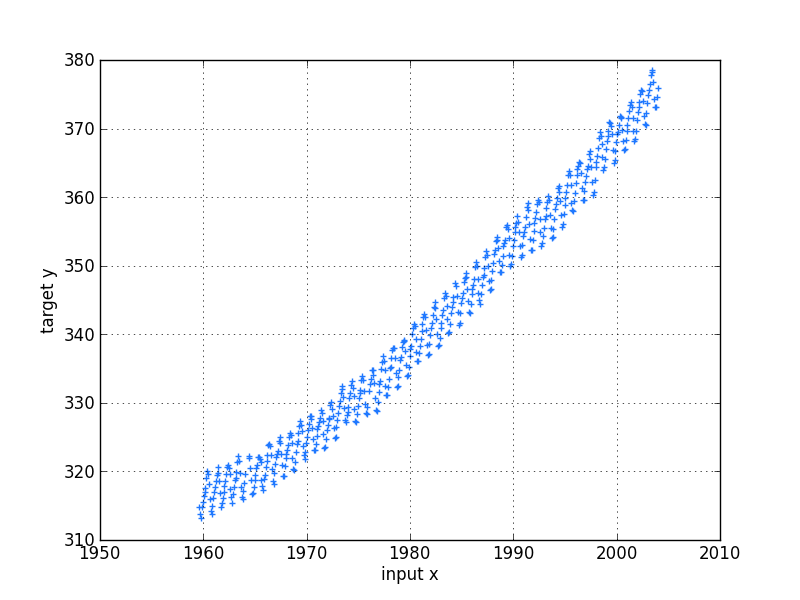
\includegraphics{_images/demoML1.png}}
\end{figure}

The data is shown in the above plot. Our goal is to model the $CO_2$
concentration as a function of time $t$. Several features are
immediately apparent: a long term rising trend, a pronounced seasonal variation
and some smaller irregularities. In the following, contributions to a
combined covariance function which takes care of these individual properties are suggessted.
This is meant primarily to illustrate the power and flexibility of the Gaussian
process framework—it is possible that other choices would be more appropriate
for this data set.

To model the long term smooth rising trend, a squared exponential
(SE) covariance term with two hyperparameters controlling the amplitude $\theta_1$
and characteristic length-scale $\theta_2$ is used:
\begin{gather}
\begin{split}k_1(x,x') = \theta_1^2 \exp \left(-\frac{(x-x')^2}{2\theta_2^2}\right).\end{split}\notag\\\begin{split}\end{split}\notag
\end{gather}
Note that we just use a smooth trend; actually enforcing the trend \emph{a priori} to be increasing
is probably not so simple and (hopefully) not desirable. We can use the periodic covariance function with a period of one year to
model the seasonal variation. However, it is not clear that the seasonal trend is
exactly periodic, so we modify it by taking the product with a squared
exponential component to allow a decay away from exact periodicity:
\begin{gather}
\begin{split}k_2(x,x') = \theta_3^2 \exp\left(-\frac{(x-x')^2}{2\theta_4^2}  \frac{2\sin^2(\pi(x-x'))}{\theta_5^2}\right).\end{split}\notag
\end{gather}
where $\theta_3$ gives the magnitude, $\theta_4$ the decay-time for the periodic component, and
$\theta_5$ the smoothness of the periodic component; the period has been fixed
to one (year). The seasonal component in the data is caused primarily by
different rates of $CO_2$ uptake for plants depending on the season, and it is
probably reasonable to assume that this pattern may itself change slowly over
time, partially due to the elevation of the $CO_2$
level itself; if this effect turns out not to be relevant, then it can be effectively removed at the fitting stage by
allowing $\theta_4$ to become very large.

To model the (small) medium term irregularities, a rational quadratic term is used:
\begin{gather}
\begin{split}k_3(x,x') = \theta_6^2\left(1+\frac{(x-x')^2}{2\theta_8\theta_7^2}\right)^{\theta_8}.\end{split}\notag
\end{gather}
where $\theta_6$ is the magnitude, $\theta_7$
is the typical length-scale and $\theta_8$ is the shape parameter determining diffuseness of the length-scales.

One could also have used a squared exponential form for this component,
but it turns out that the rational quadratic works better (gives higher marginal
likelihood), probably because it can accommodate several length-scales simultaneously.

Finally we specify a noise model as the sum of a squared exponential contrubition and an independent component:
\begin{gather}
\begin{split}k_4(x_p,x_q) = \theta_9^2\exp\left(-\frac{(x_p - x_q)^2}{2\theta_{10}^2}\right) + \theta_{11}^2\delta_{pq}.\end{split}\notag
\end{gather}
where $\theta_9$ is the magnitude of the correlated noise component, $\theta_{10}$
is its length scale and $\theta_{11}$ is the magnitude of the independent noise component. Noise in
the series could be caused by measurement inaccuracies, and by local short-term
weather phenomena, so it is probably reasonable to assume at least a modest
amount of correlation in time. Notice that the correlated noise component, the
first term has an identical expression to the long term component
in the trend covariance. When optimizing the hyperparameters, we will see that one of
these components becomes large with a long length-scale (the long term trend),
while the other remains small with a short length-scale (noise). The fact that
we have chosen to call one of these components ‘signal’ and the other one ‘noise’
is only a question of interpretation. Presumably, we are less interested in very
short-term effect, and thus call it noise; if on the other hand we were interested
in this effect, we would call it signal.

The final covariance function is:
\begin{gather}
\begin{split}k(x,x') = k_1(x,x') + k_2(x,x') + k_3(x,x') + k_4(x,x')\end{split}\notag
\end{gather}
with hyperparameters $\theta = (\theta_1,\ldots,\theta_{11})$

\begin{Verbatim}[commandchars=\\\{\}]
\PYG{c}{\PYGZsh{} DEFINE parameterized covariance function}
\PYG{n}{k1} \PYG{o}{=} \PYG{n}{cov}\PYG{o}{.}\PYG{n}{RBF}\PYG{p}{(}\PYG{n}{np}\PYG{o}{.}\PYG{n}{log}\PYG{p}{(}\PYG{l+m+mf}{67.}\PYG{p}{)}\PYG{p}{,} \PYG{n}{np}\PYG{o}{.}\PYG{n}{log}\PYG{p}{(}\PYG{l+m+mf}{66.}\PYG{p}{)}\PYG{p}{)}
\PYG{n}{k2} \PYG{o}{=} \PYG{n}{cov}\PYG{o}{.}\PYG{n}{Periodic}\PYG{p}{(}\PYG{n}{np}\PYG{o}{.}\PYG{n}{log}\PYG{p}{(}\PYG{l+m+mf}{1.3}\PYG{p}{)}\PYG{p}{,} \PYG{n}{np}\PYG{o}{.}\PYG{n}{log}\PYG{p}{(}\PYG{l+m+mf}{1.0}\PYG{p}{)}\PYG{p}{,} \PYG{n}{np}\PYG{o}{.}\PYG{n}{log}\PYG{p}{(}\PYG{l+m+mf}{2.4}\PYG{p}{)}\PYG{p}{)} \PYG{o}{*} \PYG{n}{cov}\PYG{o}{.}\PYG{n}{RBF}\PYG{p}{(}\PYG{n}{np}\PYG{o}{.}\PYG{n}{log}\PYG{p}{(}\PYG{l+m+mf}{90.}\PYG{p}{)}\PYG{p}{,} \PYG{n}{np}\PYG{o}{.}\PYG{n}{log}\PYG{p}{(}\PYG{l+m+mf}{2.4}\PYG{p}{)}\PYG{p}{)}
\PYG{n}{k3} \PYG{o}{=} \PYG{n}{cov}\PYG{o}{.}\PYG{n}{RQ}\PYG{p}{(}\PYG{n}{np}\PYG{o}{.}\PYG{n}{log}\PYG{p}{(}\PYG{l+m+mf}{1.2}\PYG{p}{)}\PYG{p}{,} \PYG{n}{np}\PYG{o}{.}\PYG{n}{log}\PYG{p}{(}\PYG{l+m+mf}{0.66}\PYG{p}{)}\PYG{p}{,} \PYG{n}{np}\PYG{o}{.}\PYG{n}{log}\PYG{p}{(}\PYG{l+m+mf}{0.78}\PYG{p}{)}\PYG{p}{)}
\PYG{n}{k4} \PYG{o}{=} \PYG{n}{cov}\PYG{o}{.}\PYG{n}{RBF}\PYG{p}{(}\PYG{n}{np}\PYG{o}{.}\PYG{n}{log}\PYG{p}{(}\PYG{l+m+mf}{1.6}\PYG{o}{/}\PYG{l+m+mf}{12.}\PYG{p}{)}\PYG{p}{,} \PYG{n}{np}\PYG{o}{.}\PYG{n}{log}\PYG{p}{(}\PYG{l+m+mf}{0.18}\PYG{p}{)}\PYG{p}{)} \PYG{o}{+} \PYG{n}{cov}\PYG{o}{.}\PYG{n}{Noise}\PYG{p}{(}\PYG{n}{np}\PYG{o}{.}\PYG{n}{log}\PYG{p}{(}\PYG{l+m+mf}{0.19}\PYG{p}{)}\PYG{p}{)}
\PYG{n}{k}  \PYG{o}{=} \PYG{n}{k1} \PYG{o}{+} \PYG{n}{k2} \PYG{o}{+} \PYG{n}{k3} \PYG{o}{+} \PYG{n}{k4}
\end{Verbatim}

After running the minimization,

\begin{Verbatim}[commandchars=\\\{\}]
\PYG{n}{t0} \PYG{o}{=} \PYG{n}{clock}\PYG{p}{(}\PYG{p}{)}
\PYG{n}{model}\PYG{o}{.}\PYG{n}{train}\PYG{p}{(}\PYG{n}{x}\PYG{p}{,}\PYG{n}{y}\PYG{p}{)}
\PYG{n}{t1} \PYG{o}{=} \PYG{n}{clock}\PYG{p}{(}\PYG{p}{)}
\PYG{n}{model}\PYG{o}{.}\PYG{n}{predict}\PYG{p}{(}\PYG{n}{xs}\PYG{p}{)}
\end{Verbatim}

The extrapolated data looks like:
\begin{figure}[htbp]
\centering

\scalebox{0.700000}{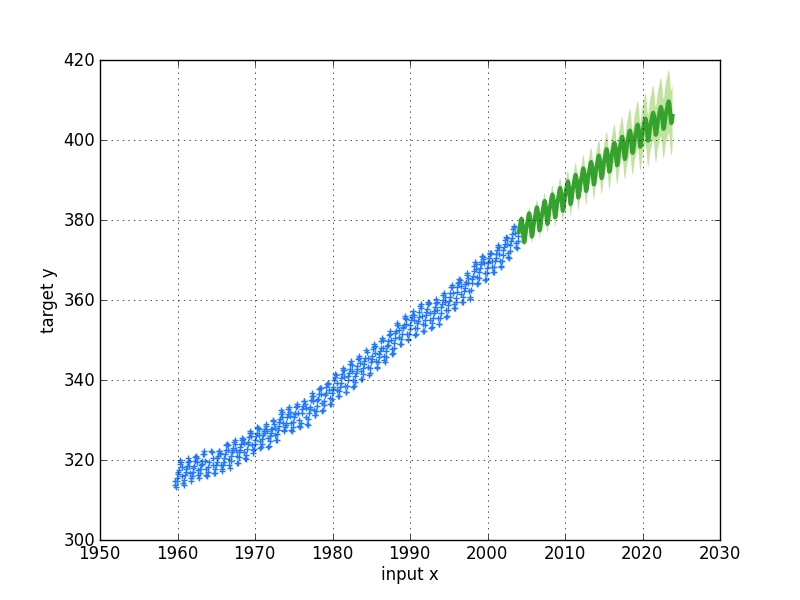
\includegraphics{_images/demoML2.png}}
\end{figure}

and the optimized values of the hyperparameters allow for a principled analysis of different components driving the model.


\subsubsection{Regression on UCI Housing data}
\label{demoHousing::doc}\label{demoHousing:regression-on-uci-housing-data}\label{demoHousing:gpml}
Boston Housing is a fairly standard dataset used for testing regression problems. It contains 506 data points with 12 numeric attributes, and one binary
categorical attribute.  The goal is to determine median home values, based on various census attributes. This dataset is available at the \href{http://archive.ics.uci.edu/ml/datasets/Housing}{UCI
Repository}.

The demo follows that in \footnote{\begin{enumerate}
\setcounter{enumi}{19}
\item {} 
Suttorp and C. Igel, Approximation of Gaussian process regression models after training. In M. Verleysen (Hrsg.), Proceedings of the 16th European Symposium on Artificial Neural Networks (ESANN 2008) , pp. 427–432 (2008).

\end{enumerate}
}.  The data set was preprocessed as follows: each continuous feature was transformed to zero mean and
unit variance (The categorical variable was dropped).  The data was partitioned into $481$ points for training and $25$ points for testing.

The mean function used was \code{src.Core.means.meanZero()} and the covariance (using the \code{src.Core.kernels.covSum()} function) was a composite of
\code{src.Core.kernels.covSEiso()} and \code{src.Core.kernels.covNoise()}.  The initial values of the hyperparameters were selected randomly from a zero-mean,
unit-variance normal distribtion.  The actual values were: $[ -0.75, \; 0.59, \; -0.45 ]$. The initial likelihood hyperparameter
was $-2.30$.  The regression started with initial negative log marginal likelihood of :math:{}` 752.46{}`.  Note the initial zero mean and the
variance that is uniform over the test set.

\begin{Verbatim}[commandchars=\\\{\}]
\PYG{n}{model} \PYG{o}{=} \PYG{n}{gp}\PYG{o}{.}\PYG{n}{GPR}\PYG{p}{(}\PYG{p}{)}
\PYG{n}{model}\PYG{o}{.}\PYG{n}{train}\PYG{p}{(}\PYG{n}{x}\PYG{p}{,}\PYG{n}{y}\PYG{p}{)}
\PYG{n}{ym}\PYG{p}{,} \PYG{n}{ys2}\PYG{p}{,} \PYG{n}{fm}\PYG{p}{,} \PYG{n}{fs2}\PYG{p}{,} \PYG{n}{lp} \PYG{o}{=} \PYG{n}{model}\PYG{o}{.}\PYG{n}{predict}\PYG{p}{(}\PYG{n}{xs}\PYG{p}{)}
\PYG{n}{xa}  \PYG{o}{=} \PYG{n}{np}\PYG{o}{.}\PYG{n}{concatenate}\PYG{p}{(}\PYG{p}{(}\PYG{n}{data}\PYG{p}{[}\PYG{p}{:}\PYG{p}{,}\PYG{p}{:}\PYG{l+m+mi}{4}\PYG{p}{]}\PYG{p}{,}\PYG{n}{data}\PYG{p}{[}\PYG{p}{:}\PYG{p}{,}\PYG{l+m+mi}{5}\PYG{p}{:}\PYG{o}{-}\PYG{l+m+mi}{1}\PYG{p}{]}\PYG{p}{)}\PYG{p}{,}\PYG{n}{axis}\PYG{o}{=}\PYG{l+m+mi}{1}\PYG{p}{)}
\PYG{n}{xa} \PYG{o}{=} \PYG{p}{(}\PYG{n}{xa} \PYG{o}{-} \PYG{n}{np}\PYG{o}{.}\PYG{n}{mean}\PYG{p}{(}\PYG{n}{xa}\PYG{p}{,}\PYG{n}{axis}\PYG{o}{=}\PYG{l+m+mi}{0}\PYG{p}{)}\PYG{p}{)}\PYG{o}{/}\PYG{p}{(}\PYG{n}{np}\PYG{o}{.}\PYG{n}{std}\PYG{p}{(}\PYG{n}{xa}\PYG{p}{,}\PYG{n}{axis}\PYG{o}{=}\PYG{l+m+mi}{0}\PYG{p}{)}\PYG{o}{+}\PYG{l+m+mf}{1.e-16}\PYG{p}{)}
\PYG{n}{ya}\PYG{p}{,} \PYG{n}{ys2a}\PYG{p}{,} \PYG{n}{fma}\PYG{p}{,} \PYG{n}{fs2a}\PYG{p}{,} \PYG{n}{lpa} \PYG{o}{=} \PYG{n}{model}\PYG{o}{.}\PYG{n}{predict}\PYG{p}{(}\PYG{n}{xa}\PYG{p}{)}
\end{Verbatim}
\begin{figure}[htbp]
\centering

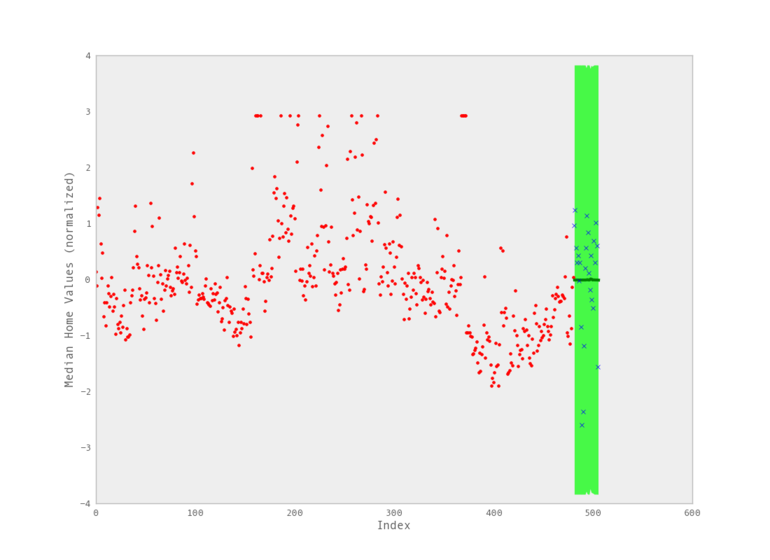
\includegraphics[width=600pt,height=300pt]{_images/demoH1.png}
\end{figure}

After hyperparameter optimization, the covariance hyperparameters were $[ 1.17, \;  0.45, \; -1.41 ]$ and the likelihood
hyperparameter was $-2.27$.  The final negative log marginal likelihood (optimized) was  $214.46$.
\begin{figure}[htbp]
\centering

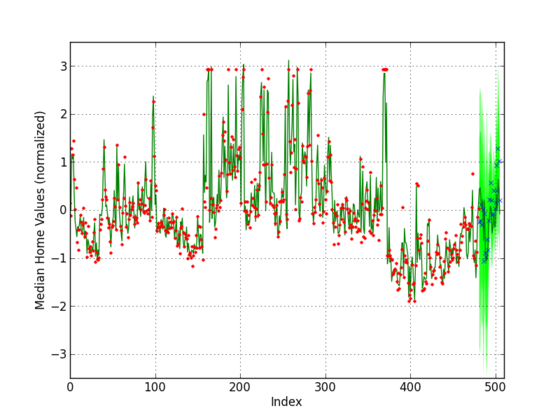
\includegraphics[width=600pt,height=300pt]{_images/demoH2.png}
\end{figure}


\subsubsection{Semi-supervised Learning with Graphs}
\label{SemiSupervised:semi-supervised-learning-with-graphs}\label{SemiSupervised::doc}
The code shown in this tutorial can be executed by running \emph{pyGPs/Demo/demo\_KernelOnGraph.py}


\paragraph{Load data}
\label{SemiSupervised:load-data}
We used the same dataset from GPMC example. i.e. The USPS digits dataset \footnote{
A Database for Handwritten Text Recognition Research, J. J. Hull, IEEE PAMI 16(5) 550-554, 1994.
}.
Each digit of $16*16$ pixels is flattened into a $256$ dimension vector.
For the simplicity of demo, we only selected digits $1$ s and $2$ s such that we have a binary classification problem where digit $1$ for class +1 and digit $2$ for class -1. We also reduced the dataset into $100$ samples per digit, where the original dataset consist of thousands of samples for each digit.

Here are samples for two digits for $1$

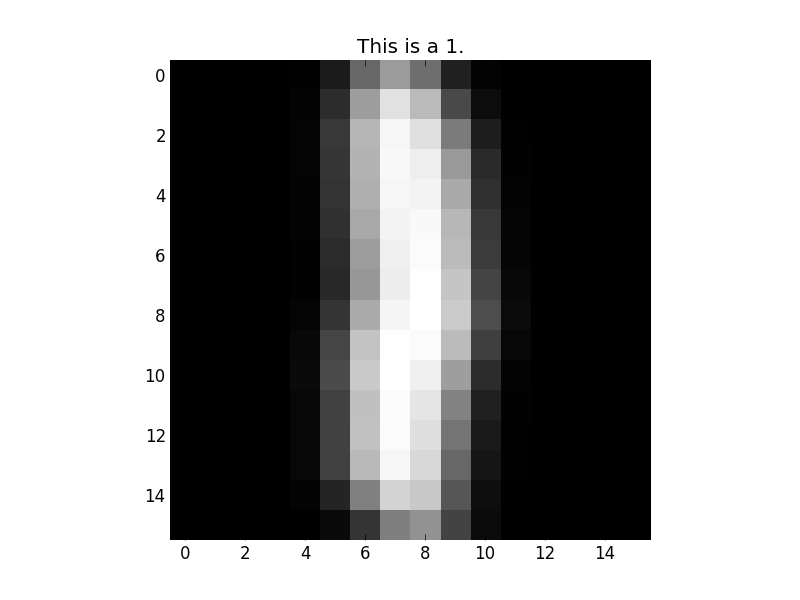
\includegraphics[width=0.300\linewidth]{_images/digit1_1.png}

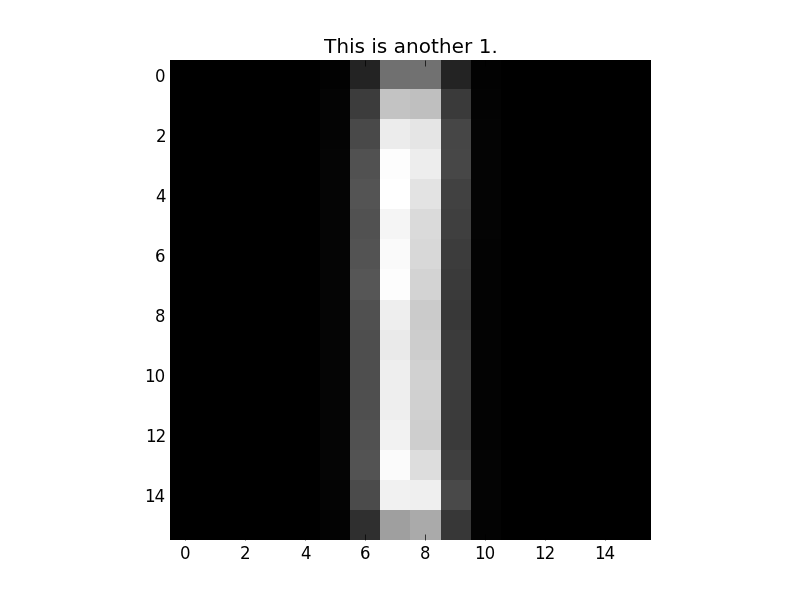
\includegraphics[width=0.300\linewidth]{_images/digit1_2.png}

and samples for two digits for $2$

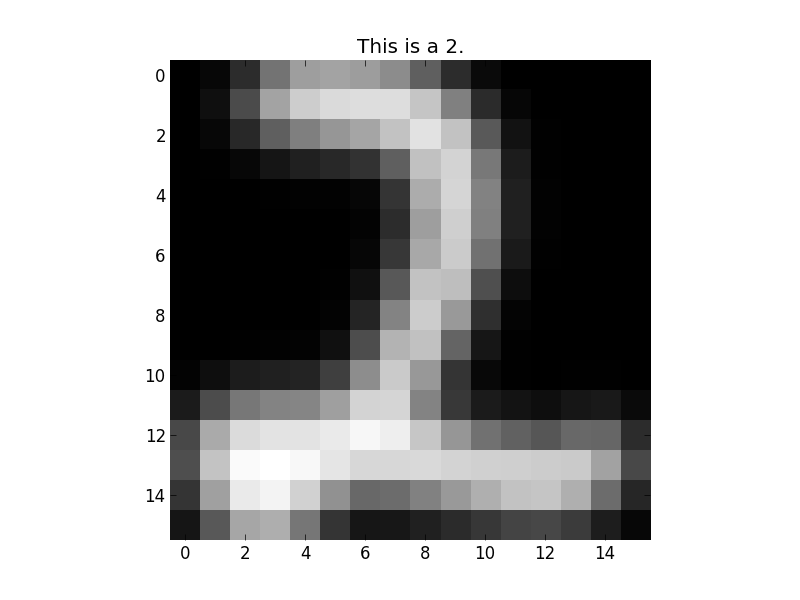
\includegraphics[width=0.300\linewidth]{_images/digit2_1.png}

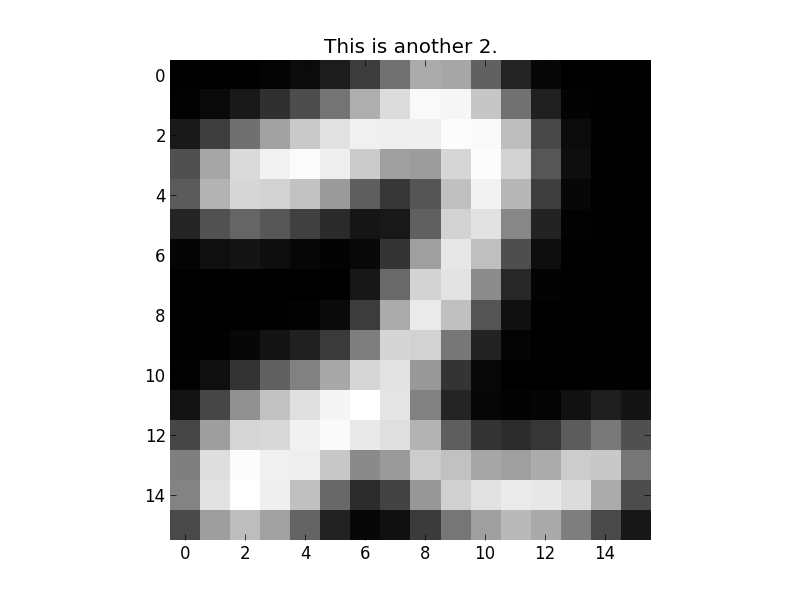
\includegraphics[width=0.300\linewidth]{_images/digit2_2.png}


\paragraph{Form a nearest neighbour graph}
\label{SemiSupervised:form-a-nearest-neighbour-graph}
We form a nearest-neighbor graph based on Euclidean distance of the vector representation of digits. Neighboring images have small Euclidean distance. Each digit is a node in the graph. There is an edge if digit $i$ is the k-nearest neighbour of digit $j$. We form a symmetrized graph such that we connect nodes $j$, $i$ if i is in j’s kNN and vice versa, and therefore a node can have more than k edges. You should import the corresponding module from \emph{pyGPs.GraphStuff}

\begin{Verbatim}[commandchars=\\\{\}]
\PYG{n}{x}\PYG{p}{,}\PYG{n}{y} \PYG{o}{=} \PYG{n}{load\PYGZus{}binary}\PYG{p}{(}\PYG{l+m+mi}{1}\PYG{p}{,}\PYG{l+m+mi}{2}\PYG{p}{,}\PYG{n+nb}{reduce}\PYG{o}{=}\PYG{n+nb+bp}{True}\PYG{p}{)}
\PYG{n}{A} \PYG{o}{=} \PYG{n}{form\PYGZus{}knn\PYGZus{}graph}\PYG{p}{(}\PYG{n}{x}\PYG{p}{,}\PYG{l+m+mi}{2}\PYG{p}{)}
\end{Verbatim}

A is the adjacency matrix of this $2-NN$ graph.

Below shows an example of such symmetrized Euclidean $2-NN$ graph on some 1s and 2s taking from Xiaojin Zhu's doctoral thesis \footnote{
Semi-Supervised Learning with Graphs, Xiaojin Zhu, CMU-LTI-05-192, 2005
}.
\begin{figure}[htbp]
\centering

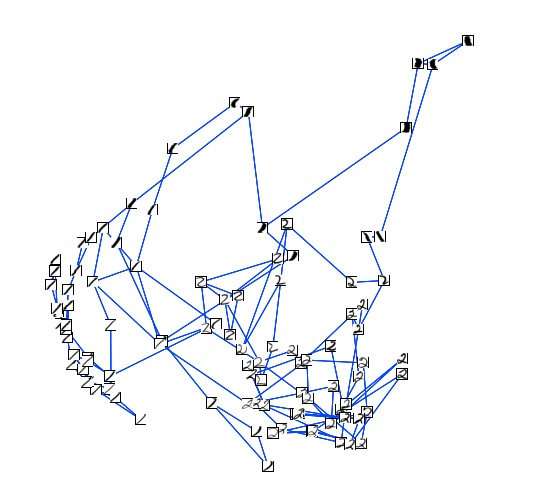
\includegraphics{_images/2nnGraph.png}
\end{figure}


\paragraph{Kernel on graph}
\label{SemiSupervised:kernel-on-graph}
Several classical kernels on graph described in Structured Kernels can be built from adjacency matrix $A$. We use diffusion kernel for this example to get the precomputed kernel matrix.

\begin{Verbatim}[commandchars=\\\{\}]
\PYG{n}{Matrix} \PYG{o}{=} \PYG{n}{diffKernel}\PYG{p}{(}\PYG{n}{A}\PYG{p}{)}
\end{Verbatim}

This a big square matrix with all rows and columns of the number of data points.
By specifying the indice of training data and test data, we will form two matrix M1 and M2 with the exact format which \emph{pyGPs.Core.cov.Pre} needed.

\begin{Verbatim}[commandchars=\\\{\}]
\PYG{n}{M1}\PYG{p}{,}\PYG{n}{M2} \PYG{o}{=} \PYG{n}{form\PYGZus{}kernel\PYGZus{}matrix}\PYG{p}{(}\PYG{n}{Matrix}\PYG{p}{,} \PYG{n}{indice\PYGZus{}train}\PYG{p}{,} \PYG{n}{indice\PYGZus{}test}\PYG{p}{)}
\end{Verbatim}
\begin{description}
\item[{M1 is a matrix with shape \textbf{number of training points plus 1} by \textbf{number of test points}}] \leavevmode\begin{itemize}
\item {} 
cross covariances matrix (train by test)

\item {} 
last row is self covariances (diagonal of test by test)

\end{itemize}

\item[{M2 is a square matrix with \textbf{number of training points} for each dimension}] \leavevmode\begin{itemize}
\item {} 
training set covariance matrix (train by train)

\end{itemize}

\end{description}


\paragraph{GP classification}
\label{SemiSupervised:gp-classification}
Every ingredients for a basic semi-supervised learning is prepared now.  Lets see how to proceed for $GP$ classification. First, the normal way with rbf kernel we have seen several times

\begin{Verbatim}[commandchars=\\\{\}]
\PYG{n}{model} \PYG{o}{=} \PYG{n}{gp}\PYG{o}{.}\PYG{n}{GPC}\PYG{p}{(}\PYG{p}{)}
\PYG{n}{k} \PYG{o}{=} \PYG{n}{cov}\PYG{o}{.}\PYG{n}{RBF}\PYG{p}{(}\PYG{p}{)}
\PYG{n}{model}\PYG{o}{.}\PYG{n}{setPrior}\PYG{p}{(}\PYG{n}{kernel}\PYG{o}{=}\PYG{n}{k}\PYG{p}{)}
\end{Verbatim}

Then lets use our kernel precomputed matrix. If you only use precomputed kernel matrix, there is no training data.
However you still need to specify $x$ just to fit in the usage of pyGPs for generality reason.
You can create any $x$ as long as the dimension is correct.

\begin{Verbatim}[commandchars=\\\{\}]
\PYG{n}{x} \PYG{o}{=} \PYG{n}{np}\PYG{o}{.}\PYG{n}{zeros}\PYG{p}{(}\PYG{p}{(}\PYG{n}{n}\PYG{p}{,}\PYG{l+m+mi}{1}\PYG{p}{)}\PYG{p}{)}
\PYG{n}{k} \PYG{o}{=} \PYG{n}{cov}\PYG{o}{.}\PYG{n}{Pre}\PYG{p}{(}\PYG{n}{M1}\PYG{p}{,}\PYG{n}{M2}\PYG{p}{)} \PYG{o}{+} \PYG{n}{cov}\PYG{o}{.}\PYG{n}{RBF}\PYG{p}{(}\PYG{p}{)}
\PYG{n}{model}\PYG{o}{.}\PYG{n}{setPrior}\PYG{p}{(}\PYG{n}{kernel}\PYG{o}{=}\PYG{n}{k}\PYG{p}{)}
\end{Verbatim}

Moreover, you can composite a kernel for both precomputed matrix and regular kernel function if necessary.

\begin{Verbatim}[commandchars=\\\{\}]
\PYG{n}{k} \PYG{o}{=} \PYG{n}{cov}\PYG{o}{.}\PYG{n}{Pre}\PYG{p}{(}\PYG{n}{M1}\PYG{p}{,}\PYG{n}{M2}\PYG{p}{)} \PYG{o}{+} \PYG{n}{cov}\PYG{o}{.}\PYG{n}{RBFunit}\PYG{p}{(}\PYG{p}{)}
\PYG{n}{model}\PYG{o}{.}\PYG{n}{setPrior}\PYG{p}{(}\PYG{n}{kernel}\PYG{o}{=}\PYG{n}{k}\PYG{p}{)}
\end{Verbatim}

The rest way of using pyGPs is exactly the same as the demo of GP classification.


\paragraph{Result}
\label{SemiSupervised:result}
For our manually created graph data, an rbf kernel works better than a diffusion kernel on the graph (higher accuracy). The performance in general should depend on the application as well as features of data.

The left image shows the digit that using diffusion kernel will predict the wrong result (should be $2$),
but rbf kernel does the job fine. The right image shows the digit that rbf kernel predicts the wrong class, diffusion kernel on the other hand, predicts correctly due to graph information! (should be $1$).

Interestingly, using a composite kernel with diffusion kernel on graph and an rbf kernel together. All test cases including the following are predicted correctly.

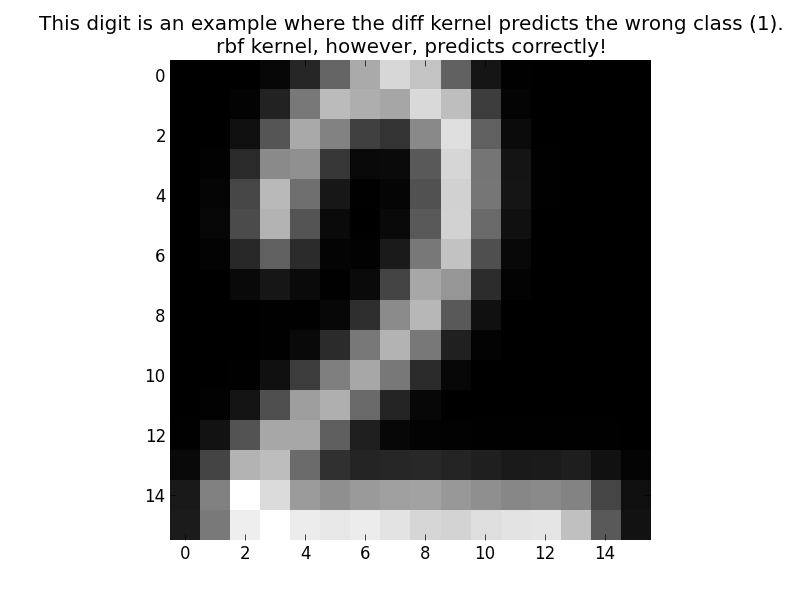
\includegraphics[width=0.500\linewidth]{_images/digitDiffwrong.png}

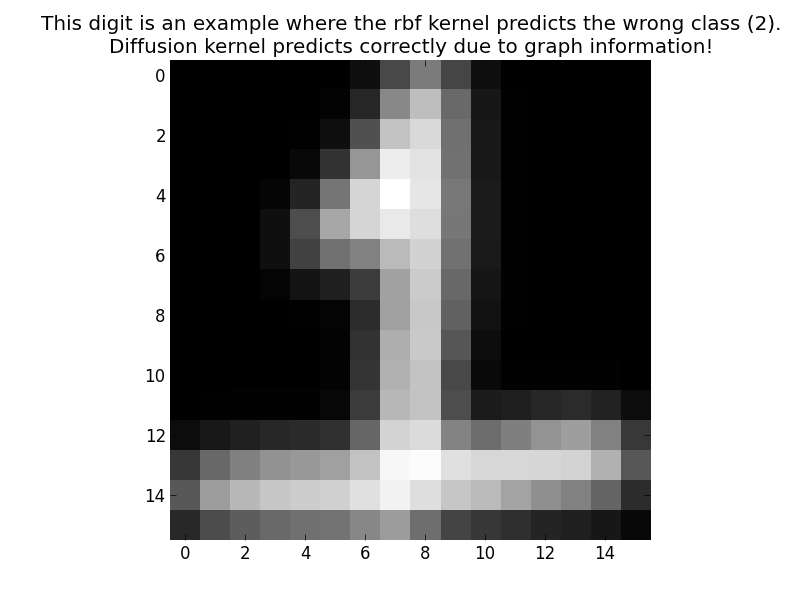
\includegraphics[width=0.500\linewidth]{_images/digitRBFwrong.png}


\section{GP functionality}
\label{index:gp-functionality}

\subsection{A brief overview of pyGPs functionality}
\label{functionality:a-brief-overview-of-pygps-functionality}\label{functionality::doc}
For detailed documentations see the API, tutorials, and respective modules/functions.


\subsubsection{kernel functions:}
\label{functionality:kernel-functions}\begin{itemize}
\item {} 
simple kernel functions:

\end{itemize}

\begin{tabulary}{\linewidth}{|L|L|}
\hline

Poly
 & 
Polynomial kernel
\\\hline

PiecePoly
 & 
Piecewise polynomial kernel with compact support
\\\hline

RBF
 & 
Squared Exponential kernel
\\\hline

RBFunit
 & 
Squared Exponential kernel with unit magnitude
\\\hline

RBFard
 & 
Squared Exponential kernel with Automatic Relevance Determination
\\\hline

Const
 & 
Constant kernel
\\\hline

Linear
 & 
Linear kernel
\\\hline

LINard
 & 
Linear covariance function with Automatic Relevance Detemination
\\\hline

Matern
 & 
Matern covariance function
\\\hline

Periodic
 & 
Stationary kernel for a smooth periodic function
\\\hline

Noise
 & 
Independent covariance function, i.e ``white noise''
\\\hline

RQ
 & 
Rational Quadratic covariance function with isotropic distance measure
\\\hline

RQard
 & 
Rational Quadratic covariance function with ARD distance measure
\\\hline

Pre
 & 
Precomputed kernel matrix
\\\hline
\end{tabulary}

\begin{itemize}
\item {} 
composite kernel functions:

\end{itemize}

\begin{tabulary}{\linewidth}{|L|L|}
\hline

ProductOfKernel or ``*''
 & 
product of covariance functions
\\\hline

ScaleOfKernel or ``*''
 & 
scale covariance function (by scalar)
\\\hline

SumOfKernel or ``+''
 & 
sum of (parameterized) covariance functions
\\\hline

FITCOfKernel
 & 
covariance function to be used together with the FITC approximation
\\\hline
\end{tabulary}



\subsubsection{mean functions:}
\label{functionality:mean-functions}\begin{itemize}
\item {} 
simple mean functions:

\end{itemize}

\begin{tabulary}{\linewidth}{|L|L|}
\hline

Zero
 & 
zero mean function
\\\hline

One
 & 
one mean function
\\\hline

Const
 & 
constant mean function
\\\hline

Linear
 & 
linear mean function
\\\hline
\end{tabulary}

\begin{itemize}
\item {} 
composite covariance functions:

\end{itemize}

\begin{tabulary}{\linewidth}{|L|L|}
\hline

ProductOfMean or ``*''
 & 
products of mean functions
\\\hline

SumOfMean or ``+''
 & 
sums of mean functions
\\\hline

ScaleOfMean ``*''
 & 
scaled version of a mean function
\\\hline

PowerOfMean ``**''
 & 
power of a mean function
\\\hline
\end{tabulary}



\subsubsection{lik functions:}
\label{functionality:lik-functions}
\begin{tabulary}{\linewidth}{|L|L|}
\hline

Erf
 & 
Error function, classification, probit regression
\\\hline

Gauss
 & 
Gaussian likelihood function for regression
\\\hline

Laplace
 & 
Laplacian likelihood function for regression
\\\hline
\end{tabulary}



\subsubsection{inf functions:}
\label{functionality:inf-functions}
\begin{tabulary}{\linewidth}{|L|L|}
\hline

Exact
 & 
Exact inference (only possible with Gaussian likelihood)
\\\hline

EP
 & 
Expectation Propagation
\\\hline

Laplace
 & 
Laplace's Approximation
\\\hline

FITC\_Exact
 & 
Large scale regression with approximate covariance matrix
\\\hline

FITC\_EP
 & 
Large scale inference  with approximate covariance matrix
\\\hline

FITC\_Laplace
 & 
Large scale inference  with approximate covariance matrix
\\\hline
\end{tabulary}



\subsubsection{optimization methods:}
\label{functionality:optimization-methods}
\begin{tabulary}{\linewidth}{|L|L|}
\hline

Minimize
 & 
Minimize by Carl Rasmussen
\\\hline

CG
 & 
Conjugent gradient
\\\hline

BFGS
 & 
Quasi-Newton method of Broyden, Fletcher, Goldfarb, and Shanno (BFGS)
\\\hline

SCG
 & 
Scaled conjugent gradient (faster than CG)
\\\hline
\end{tabulary}



\subsubsection{evaluation measures:}
\label{functionality:evaluation-measures}
\begin{tabulary}{\linewidth}{|L|L|}
\hline

RMSE
 & 
Root mean squared error
\\\hline

ACC
 & 
Classification accuracy
\\\hline

Prec
 & 
Precision for class +1
\\\hline

Recall
 & 
Recall for class +1
\\\hline

NLPD
 & 
Negative log predictive density in transformed observation space
\\\hline
\end{tabulary}



\subsection{Kernels \& Means}
\label{Kernels:kernels-means}\label{Kernels::doc}

\subsubsection{Simple Kernel \& Mean}
\label{Kernels:simple-kernel-mean}
You may already seen, we can specify a kernel function like this(same for mean fucntions):

\begin{Verbatim}[commandchars=\\\{\}]
\PYG{n}{k} \PYG{o}{=} \PYG{n}{cov}\PYG{o}{.}\PYG{n}{RBF}\PYG{p}{(} \PYG{n}{log\PYGZus{}ell}\PYG{o}{=}\PYG{o}{-}\PYG{l+m+mf}{1.}\PYG{p}{,} \PYG{n}{log\PYGZus{}sigma}\PYG{o}{=}\PYG{l+m+mf}{0.} \PYG{p}{)}
\end{Verbatim}

There are several points need to be noticed:
\begin{enumerate}
\item {} 
Most parameters are initilized in their logorithms. This is because we need to make sure they are positive during optimization. e.g. Here length scale and signal variance should always be positive.

\item {} 
Most kernel functions have a scalar in front, namely signal variance(set by log\_sigma)

\item {} 
If you will do optimization later anyway, you can just leave parameters to be default

\end{enumerate}


\subsubsection{Some Special Cases}
\label{Kernels:some-special-cases}\begin{enumerate}
\item {} 
For some kernels/means, number of hyperparameters depends on the dimension of input data.
You can either enter the dimension, which use default values:

\begin{Verbatim}[commandchars=\\\{\}]
\PYG{n}{m} \PYG{o}{=} \PYG{n}{mean}\PYG{o}{.}\PYG{n}{Linear}\PYG{p}{(} \PYG{n}{D}\PYG{o}{=}\PYG{n}{x}\PYG{o}{.}\PYG{n}{shape}\PYG{p}{[}\PYG{l+m+mi}{1}\PYG{p}{]} \PYG{p}{)}
\end{Verbatim}

or you can initialze with the exact hyperparameters,
you should enter as a list, one element for each dimension

\begin{Verbatim}[commandchars=\\\{\}]
\PYG{n}{m} \PYG{o}{=} \PYG{n}{mean}\PYG{o}{.}\PYG{n}{Linear}\PYG{p}{(} \PYG{n}{alpha\PYGZus{}list}\PYG{o}{=}\PYG{p}{[}\PYG{l+m+mf}{0.2}\PYG{p}{,} \PYG{l+m+mf}{0.4}\PYG{p}{,} \PYG{l+m+mf}{0.3}\PYG{p}{]} \PYG{p}{)}
\end{Verbatim}
\begin{description}
\item[{All these ``hyp-dim-dependent'' functions are:}] \leavevmode\begin{itemize}
\item {} 
\emph{mean.Linear}

\item {} 
\emph{cov.RBFard}

\item {} 
\emph{cov.LINard}

\item {} 
\emph{cov.RQard}

\end{itemize}

\end{description}

\item {} 
For linear kernel, there is NO signal variance(scalar) in front of the function.

If you want to add a scalar for it, you can use:

\begin{Verbatim}[commandchars=\\\{\}]
\PYG{n}{k} \PYG{o}{=} \PYG{l+m+mf}{0.5} \PYG{o}{*} \PYG{n}{cov}\PYG{o}{.}\PYG{n}{LIN}\PYG{p}{(}\PYG{p}{)}
\end{Verbatim}

If you also want to add a bias term:

\begin{Verbatim}[commandchars=\\\{\}]
\PYG{n}{k} \PYG{o}{=} \PYG{l+m+mf}{0.5} \PYG{o}{*} \PYG{n}{cov}\PYG{o}{.}\PYG{n}{LIN}\PYG{p}{(}\PYG{p}{)} \PYG{o}{+} \PYG{n}{cov}\PYG{o}{.}\PYG{n}{Const}\PYG{p}{(}\PYG{n}{c}\PYG{o}{=}\PYG{l+m+mf}{1.}\PYG{p}{)}
\end{Verbatim}

Note 0.5 will also be treated as a hyperparameter.
This also applies in \emph{cov.LINard}.

\item {} 
For \emph{cov.RBFunit()}, its signal variance is always 1 (because of unit magnitude). Therefore this function do not have a hyperparameter of ``signal variance''.

\item {} \begin{description}
\item[{\emph{cov.Poly()} has three parameters, where hyperparameters are:}] \leavevmode\begin{itemize}
\item {} 
c     -\textgreater{} inhomogeneous offset

\item {} 
sigma -\textgreater{} signal deviation

\end{itemize}

\item[{however,}] \leavevmode\begin{itemize}
\item {} 
d     -\textgreater{} order of polynomial
will be treated as normal parameter, i.e. will not be trained

\end{itemize}

\end{description}

\item {} 
Explicitly set \emph{cov.Noise} is not necessary, because noise are already added in likelihood.

\end{enumerate}


\subsubsection{Composite Kernels \& Meams}
\label{Kernels:composite-kernels-meams}
Adding and muliplying Kernels(Means) is really simple:

\begin{Verbatim}[commandchars=\\\{\}]
\PYG{n}{k} \PYG{o}{=} \PYG{n}{cov}\PYG{o}{.}\PYG{n}{Periodic}\PYG{p}{(}\PYG{p}{)} \PYG{o}{*} \PYG{n}{cov}\PYG{o}{.}\PYG{n}{RBF}\PYG{p}{(}\PYG{p}{)}
\PYG{n}{k} \PYG{o}{=} \PYG{l+m+mf}{0.5}\PYG{o}{*}\PYG{n}{cov}\PYG{o}{.}\PYG{n}{LIN}\PYG{p}{(}\PYG{p}{)} \PYG{o}{+} \PYG{n}{cov}\PYG{o}{.}\PYG{n}{Periodic}\PYG{p}{(}\PYG{p}{)}
\end{Verbatim}

Scalar will also be treated as a hyperparameter. For example, k = s1 * k1 + s2 * k2,
then the list of hyperparameters is hyp = {[}s1, k1.hyp, s2, k2.hyp{]}. Scalar is passed in logorithm domain such that it will always be positive during optimization.

Except linear kernel, all kernel functions have a scalar (signal variance) as hyperparameter.
Therefore, the only explict scalar might be added to cov.LIN()

Beside + / * , there is also a power operator for mean functions:

\begin{Verbatim}[commandchars=\\\{\}]
\PYG{n}{m} \PYG{o}{=} \PYG{p}{(} \PYG{n}{mean}\PYG{o}{.}\PYG{n}{One}\PYG{p}{(}\PYG{p}{)}\PYG{o}{+}\PYG{n}{mean}\PYG{o}{.}\PYG{n}{Linear}\PYG{p}{(}\PYG{n}{alpha\PYGZus{}list}\PYG{o}{=}\PYG{p}{[}\PYG{l+m+mf}{0.2}\PYG{p}{]}\PYG{p}{)} \PYG{p}{)}\PYG{o}{*}\PYG{o}{*}\PYG{l+m+mi}{2}
\end{Verbatim}


\subsubsection{Precomputed Kernel Matrix}
\label{Kernels:precomputed-kernel-matrix}
In certain cases, you may have a precomputed kernel matrix,
but its non-trivial to write down the exact formula of kernel functions. Then you can specify your kernel in the following way. A precomputed kernel also fits with other kernels. In other words, it can also be composited as the way other kernels functions do.

\begin{Verbatim}[commandchars=\\\{\}]
\PYG{n}{k} \PYG{o}{=} \PYG{n}{cov}\PYG{o}{.}\PYG{n}{Pre}\PYG{p}{(}\PYG{n}{M1}\PYG{p}{,} \PYG{n}{M2}\PYG{p}{)}
\end{Verbatim}

M1 and M2 are your precomputed kernel matrix,

where,
\begin{description}
\item[{M1 is a matrix with shape \textbf{number of training points plus 1} by \textbf{number of test points}}] \leavevmode\begin{itemize}
\item {} 
cross covariances matrix (train by test)

\item {} 
last row is self covariances (diagonal of test by test)

\end{itemize}

\item[{M2 is a square matrix with \textbf{number of training points} for each dimension}] \leavevmode\begin{itemize}
\item {} 
training set covariance matrix (train by train)

\end{itemize}

\end{description}

A precomputed kernel can also be composited with other kernels. Similar to \emph{cov.LIN()}, you need to explictly add scalar for \emph{cov.Pre()}.

\begin{Verbatim}[commandchars=\\\{\}]
\PYG{n}{k} \PYG{o}{=} \PYG{l+m+mf}{0.5}\PYG{o}{*}\PYG{n}{cov}\PYG{o}{.}\PYG{n}{Pre}\PYG{p}{(}\PYG{n}{M1}\PYG{p}{,} \PYG{n}{M2}\PYG{p}{)} \PYG{o}{+} \PYG{n}{cov}\PYG{o}{.}\PYG{n}{RBF}\PYG{p}{(}\PYG{p}{)}
\end{Verbatim}


\subsubsection{Customizing Kernel \& Mean}
\label{Kernels:customizing-kernel-mean}
We also support you to create your own kernel/mean class, your customized kernel class need to follow the structure template as below:

\begin{Verbatim}[commandchars=\\\{\}]
\PYG{c}{\PYGZsh{} Your kernel class needs to inherit base class Kernel,}
\PYG{c}{\PYGZsh{} which is in the module of Core.cov}
\PYG{k}{class} \PYG{n+nc}{MyKernel}\PYG{p}{(}\PYG{n}{Kernel}\PYG{p}{)}\PYG{p}{:}

    \PYG{k}{def} \PYG{n+nf}{\PYGZus{}\PYGZus{}init\PYGZus{}\PYGZus{}}\PYG{p}{(}\PYG{n+nb+bp}{self}\PYG{p}{,} \PYG{n}{para1}\PYG{o}{=}\PYG{l+m+mf}{0.}\PYG{p}{,} \PYG{n}{para2}\PYG{o}{=}\PYG{l+m+mf}{0.}\PYG{p}{,} \PYG{n}{para3}\PYG{o}{=}\PYG{l+m+mf}{0.}\PYG{p}{)}\PYG{p}{:}
        \PYG{n+nb+bp}{self}\PYG{o}{.}\PYG{n}{hyp} \PYG{o}{=} \PYG{p}{[}\PYG{n}{para1}\PYG{p}{,} \PYG{n}{para2}\PYG{p}{]}     \PYG{c}{\PYGZsh{} hyperparameters that can be trained}
        \PYG{n+nb+bp}{self}\PYG{o}{.}\PYG{n}{para} \PYG{o}{=} \PYG{p}{[}\PYG{n}{para3}\PYG{p}{]}           \PYG{c}{\PYGZsh{} static parameters}

    \PYG{k}{def} \PYG{n+nf}{proceed}\PYG{p}{(}\PYG{n+nb+bp}{self}\PYG{p}{,} \PYG{n}{x}\PYG{o}{=}\PYG{n+nb+bp}{None}\PYG{p}{,} \PYG{n}{z}\PYG{o}{=}\PYG{n+nb+bp}{None}\PYG{p}{,} \PYG{n}{der}\PYG{o}{=}\PYG{n+nb+bp}{None}\PYG{p}{)}\PYG{p}{:}
        \PYG{l+s+sd}{''' x is n by D training patterns matrix, and z is nn by D test case matrix'''}
        \PYG{k}{return} \PYG{n}{A}
\end{Verbatim}
\begin{description}
\item[{where the returning matrix A depends on the input:}] \leavevmode\begin{itemize}
\item {} 
if \emph{z == None}, A is covariance matrix of x with shape (n,n)

\item {} 
elif \emph{z == `diag'}, A is self covariance matrix with shape (n,1)

\item {} 
else \emph{z is a matrix (given test points)}, A is covariance between data sets x and z with shape (n,nn)

\item {} 
if \emph{der == None}, return A as defined previously.

\item {} 
else \emph{der != None}, i.e. given der as an integer der = $k$, return the derivative matrix wrt. to $k_{th}$ hyperparameter.

\end{itemize}

\end{description}

and for customized mean class:

\begin{Verbatim}[commandchars=\\\{\}]
\PYG{c}{\PYGZsh{} Your mean class needs to inherit base class Mean,}
\PYG{c}{\PYGZsh{} which is in the module of Core.mean}
\PYG{k}{class} \PYG{n+nc}{MyMean}\PYG{p}{(}\PYG{n}{Mean}\PYG{p}{)}\PYG{p}{:}

    \PYG{k}{def} \PYG{n+nf}{\PYGZus{}\PYGZus{}init\PYGZus{}\PYGZus{}}\PYG{p}{(}\PYG{n+nb+bp}{self}\PYG{p}{,} \PYG{n}{para1}\PYG{o}{=}\PYG{l+m+mf}{0.}\PYG{p}{,} \PYG{n}{para2}\PYG{o}{=}\PYG{l+m+mf}{0.}\PYG{p}{,} \PYG{n}{para3}\PYG{o}{=}\PYG{l+m+mf}{0.}\PYG{p}{)}\PYG{p}{:}
        \PYG{n+nb+bp}{self}\PYG{o}{.}\PYG{n}{hyp} \PYG{o}{=} \PYG{p}{[}\PYG{n}{para1}\PYG{p}{,} \PYG{n}{para2}\PYG{p}{]}     \PYG{c}{\PYGZsh{} hyperparameters that can be trained}
        \PYG{n+nb+bp}{self}\PYG{o}{.}\PYG{n}{para} \PYG{o}{=} \PYG{p}{[}\PYG{n}{para3}\PYG{p}{]}           \PYG{c}{\PYGZsh{} static parameters}

    \PYG{k}{def} \PYG{n+nf}{proceed}\PYG{p}{(}\PYG{n+nb+bp}{self}\PYG{p}{,} \PYG{n}{x}\PYG{o}{=}\PYG{n+nb+bp}{None}\PYG{p}{,} \PYG{n}{der}\PYG{o}{=}\PYG{n+nb+bp}{None}\PYG{p}{)}\PYG{p}{:}
        \PYG{l+s+sd}{''' x is n by D training patterns matrix'''}
        \PYG{k}{return} \PYG{n}{A}
\end{Verbatim}
\begin{description}
\item[{where the returning matrix A depends on the input:}] \leavevmode\begin{itemize}
\item {} 
if \emph{der == None}, return A as the mean of x

\item {} 
else \emph{der != None}, return the derivative of mean wrt. to $k_{th}$ hyperparameter.

\end{itemize}

\end{description}


\subsection{Likelihoods \& Inference}
\label{Likelihoods::doc}\label{Likelihoods:likelihoods-inference}

\subsubsection{Changing Likelihood \& Inference}
\label{Likelihoods:changing-likelihood-inference}\begin{description}
\item[{By default,}] \leavevmode\begin{itemize}
\item {} 
GPR uses Gaussian likelihood and exact inference.

\item {} 
GPC uses Error functionlikelihood and EP inference.

\item {} 
FITC model uses same default with corresponding FITC inference.

\item {} 
GPMC calls GPC and thus uses the default setting of GPC

\end{itemize}

\end{description}

You can change to other likelihood or inference methods using:

\begin{Verbatim}[commandchars=\\\{\}]
\PYG{n}{model}\PYG{o}{.}\PYG{n}{useLikelihood}\PYG{p}{(}\PYG{n}{newLik}\PYG{p}{)}
\PYG{n}{model}\PYG{o}{.}\PYG{n}{useInference}\PYG{p}{(}\PYG{n}{newInf}\PYG{p}{)}
\end{Verbatim}
\begin{description}
\item[{\emph{newLik} and \emph{newInf} are \textbf{Strings}. Currently the options are:}] \leavevmode\begin{enumerate}
\item {} 
Regression model
\begin{itemize}
\item {} 
newLik: \textbf{``Laplace''}. Note this will force inference method to be EP.

\item {} 
newInf: \textbf{``EP''}, \textbf{``Laplace''}.

\end{itemize}

\item {} 
Classification model (including GPMC)
\begin{itemize}
\item {} 
newInf: \textbf{``Laplace''}

\end{itemize}

\end{enumerate}

\end{description}


\subsubsection{List of Likelihoods}
\label{Likelihoods:list-of-likelihoods}\label{Likelihoods:module-pyGPs.Core.lik}\index{pyGPs.Core.lik (module)}\index{Erf (class in pyGPs.Core.lik)}

\begin{fulllineitems}
\phantomsection\label{Likelihoods:pyGPs.Core.lik.Erf}\pysigline{\strong{class }\code{pyGPs.Core.lik.}\bfcode{Erf}}
Error function or cumulative Gaussian likelihood function for binary
classification or probit regression.

$Erf(t)=\frac{1}{2}(1+erf(\frac{t}{\sqrt{2}}))=normcdf(t)$

\end{fulllineitems}

\index{Gauss (class in pyGPs.Core.lik)}

\begin{fulllineitems}
\phantomsection\label{Likelihoods:pyGPs.Core.lik.Gauss}\pysiglinewithargsret{\strong{class }\code{pyGPs.Core.lik.}\bfcode{Gauss}}{\emph{log\_sigma=-2.3025850929940455}}{}
Gaussian likelihood function for regression.

$Gauss(t)=\frac{1}{\sqrt{2\pi\sigma^2}}e^{-\frac{(t-y)^2}{2\sigma^2}}$,
where $y$ is the mean and $\sigma$ is the standard deviation.

hyp = {[} log\_sigma {]}

\end{fulllineitems}

\index{Laplace (class in pyGPs.Core.lik)}

\begin{fulllineitems}
\phantomsection\label{Likelihoods:pyGPs.Core.lik.Laplace}\pysiglinewithargsret{\strong{class }\code{pyGPs.Core.lik.}\bfcode{Laplace}}{\emph{log\_sigma=-2.3025850929940455}}{}
Laplacian likelihood function for regression. ONLY works with EP inference!

$Laplace(t) = \frac{1}{2b}e^{-\frac{|t-y|}{b}}$ where $b=\frac{\sigma}{\sqrt{2}}$,
$y$ is the mean and $\sigma$ is the standard deviation.

hyp = {[} log\_sigma {]}

\end{fulllineitems}

\index{Likelihood (class in pyGPs.Core.lik)}

\begin{fulllineitems}
\phantomsection\label{Likelihoods:pyGPs.Core.lik.Likelihood}\pysigline{\strong{class }\code{pyGPs.Core.lik.}\bfcode{Likelihood}}
Base function for Likelihood function
\index{proceed() (pyGPs.Core.lik.Likelihood method)}

\begin{fulllineitems}
\phantomsection\label{Likelihoods:pyGPs.Core.lik.Likelihood.proceed}\pysiglinewithargsret{\bfcode{proceed}}{}{}
The likelihood functions have two possible modes based on inputs. 
See lik.py for detail documentation.

\end{fulllineitems}


\end{fulllineitems}



\subsubsection{List of Inference}
\label{Likelihoods:module-pyGPs.Core.inf}\label{Likelihoods:list-of-inference}\index{pyGPs.Core.inf (module)}\index{EP (class in pyGPs.Core.inf)}

\begin{fulllineitems}
\phantomsection\label{Likelihoods:pyGPs.Core.inf.EP}\pysigline{\strong{class }\code{pyGPs.Core.inf.}\bfcode{EP}}
Expectation Propagation approximation to the posterior Gaussian Process.

\end{fulllineitems}

\index{Exact (class in pyGPs.Core.inf)}

\begin{fulllineitems}
\phantomsection\label{Likelihoods:pyGPs.Core.inf.Exact}\pysigline{\strong{class }\code{pyGPs.Core.inf.}\bfcode{Exact}}
Exact inference for a GP with Gaussian likelihood. Compute a parametrization
of the posterior, the negative log marginal likelihood and its derivatives
w.r.t. the hyperparameters.

\end{fulllineitems}

\index{FITC\_EP (class in pyGPs.Core.inf)}

\begin{fulllineitems}
\phantomsection\label{Likelihoods:pyGPs.Core.inf.FITC_EP}\pysigline{\strong{class }\code{pyGPs.Core.inf.}\bfcode{FITC\_EP}}
FITC-EP approximation to the posterior Gaussian process. The function is
equivalent to infEP with the covariance function:
Kt = Q + G; G = diag(g); g = diag(K-Q);  Q = Ku' * inv(Kuu + snu2 * eye(nu)) * Ku;
where Ku and Kuu are covariances w.r.t. to inducing inputs xu and
snu2 = sn2/1e6 is the noise of the inducing inputs. We fixed the standard
deviation of the inducing inputs snu to be a one per mil of the measurement 
noise's standard deviation sn. In case of a likelihood without noise
parameter sn2, we simply use snu2 = 1e-6.
For details, see The Generalized FITC Approximation, Andrew Naish-Guzman and
Sean Holden, NIPS, 2007.

\end{fulllineitems}

\index{FITC\_Exact (class in pyGPs.Core.inf)}

\begin{fulllineitems}
\phantomsection\label{Likelihoods:pyGPs.Core.inf.FITC_Exact}\pysigline{\strong{class }\code{pyGPs.Core.inf.}\bfcode{FITC\_Exact}}
FITC approximation to the posterior Gaussian process. The function is
equivalent to infExact with the covariance function:
Kt = Q + G; G = diag(g); g = diag(K-Q);  Q = Ku' * inv(Quu) * Ku; 
where Ku and Kuu are covariances w.r.t. to inducing inputs xu, snu2 = sn2/1e6
is the noise of the inducing inputs and Quu = Kuu + snu2*eye(nu).

\end{fulllineitems}

\index{FITC\_Laplace (class in pyGPs.Core.inf)}

\begin{fulllineitems}
\phantomsection\label{Likelihoods:pyGPs.Core.inf.FITC_Laplace}\pysigline{\strong{class }\code{pyGPs.Core.inf.}\bfcode{FITC\_Laplace}}
FITC-Laplace approximation to the posterior Gaussian process. The function is
equivalent to infLaplace with the covariance function:
Kt = Q + G; G = diag(g); g = diag(K-Q);  Q = Ku' * inv(Kuu + snu2 * eye(nu)) * Ku;
where Ku and Kuu are covariances w.r.t. to inducing inputs xu and
snu2 = sn2/1e6 is the noise of the inducing inputs. We fixed the standard
deviation of the inducing inputs snu to be a one per mil of the measurement 
noise's standard deviation sn. In case of a likelihood without noise
parameter sn2, we simply use snu2 = 1e-6.

\end{fulllineitems}

\index{Inference (class in pyGPs.Core.inf)}

\begin{fulllineitems}
\phantomsection\label{Likelihoods:pyGPs.Core.inf.Inference}\pysigline{\strong{class }\code{pyGPs.Core.inf.}\bfcode{Inference}}
Base class for inference. Defined several tool methods in it.
\index{Psi\_line() (pyGPs.Core.inf.Inference method)}

\begin{fulllineitems}
\phantomsection\label{Likelihoods:pyGPs.Core.inf.Inference.Psi_line}\pysiglinewithargsret{\bfcode{Psi\_line}}{\emph{s}, \emph{dalpha}, \emph{alpha}, \emph{K}, \emph{m}, \emph{likfunc}, \emph{y}, \emph{inffunc}}{}
Criterion Psi at alpha + s*dalpha for line search
{[}Psi,alpha,f,dlp,W{]} = Psi\_line(s,dalpha,alpha,hyp,K,m,lik,y,inf)

\end{fulllineitems}

\index{Psi\_lineFITC() (pyGPs.Core.inf.Inference method)}

\begin{fulllineitems}
\phantomsection\label{Likelihoods:pyGPs.Core.inf.Inference.Psi_lineFITC}\pysiglinewithargsret{\bfcode{Psi\_lineFITC}}{\emph{s}, \emph{dalpha}, \emph{alpha}, \emph{V}, \emph{d0}, \emph{m}, \emph{likfunc}, \emph{y}, \emph{inffunc}}{}
Criterion Psi at alpha + s*dalpha for line search

\end{fulllineitems}

\index{epfitcRefresh() (pyGPs.Core.inf.Inference method)}

\begin{fulllineitems}
\phantomsection\label{Likelihoods:pyGPs.Core.inf.Inference.epfitcRefresh}\pysiglinewithargsret{\bfcode{epfitcRefresh}}{\emph{d0}, \emph{P0}, \emph{R0}, \emph{R0P0}, \emph{w}, \emph{b}}{}
Refresh the representation of the posterior from initial and site parameters
to prevent possible loss of numerical precision after many epfitcUpdates
effort is O(n*nu\textasciicircum{}2) provided that nu\textless{}n
Sigma = inv(inv(K)+diag(W)) = diag(d) + P'{\color{red}\bfseries{}*}R0'{\color{red}\bfseries{}*}R'{\color{red}\bfseries{}*}R*R0*P.

\end{fulllineitems}

\index{epfitcZ() (pyGPs.Core.inf.Inference method)}

\begin{fulllineitems}
\phantomsection\label{Likelihoods:pyGPs.Core.inf.Inference.epfitcZ}\pysiglinewithargsret{\bfcode{epfitcZ}}{\emph{d}, \emph{P}, \emph{R}, \emph{nn}, \emph{gg}, \emph{ttau}, \emph{tnu}, \emph{d0}, \emph{R0}, \emph{P0}, \emph{y}, \emph{likfunc}, \emph{m}, \emph{inffunc}}{}
Compute the marginal likelihood approximation
effort is O(n*nu\textasciicircum{}2) provided that nu\textless{}n

\end{fulllineitems}

\index{fitcRefresh() (pyGPs.Core.inf.Inference method)}

\begin{fulllineitems}
\phantomsection\label{Likelihoods:pyGPs.Core.inf.Inference.fitcRefresh}\pysiglinewithargsret{\bfcode{fitcRefresh}}{\emph{d0}, \emph{P0}, \emph{R0}, \emph{R0P0}, \emph{w}}{}
Refresh the representation of the posterior from initial and site parameters
to prevent possible loss of numerical precision after many epfitcUpdates
effort is O(n*nu\textasciicircum{}2) provided that nu\textless{}n
Sigma = inv(inv(K)+diag(W)) = diag(d) + P'{\color{red}\bfseries{}*}R0'{\color{red}\bfseries{}*}R'{\color{red}\bfseries{}*}R*R0*P.

\end{fulllineitems}

\index{logdetA() (pyGPs.Core.inf.Inference method)}

\begin{fulllineitems}
\phantomsection\label{Likelihoods:pyGPs.Core.inf.Inference.logdetA}\pysiglinewithargsret{\bfcode{logdetA}}{\emph{K}, \emph{w}, \emph{nargout}}{}
Compute the log determinant ldA and the inverse iA of a square nxn matrix
A = eye(n) + K*diag(w) from its LU decomposition; for negative definite A, we 
return ldA = Inf. We also return mwiA = -diag(w)*inv(A).
{[}ldA,iA,mwiA{]} = logdetA(K,w)

\end{fulllineitems}

\index{mvmK() (pyGPs.Core.inf.Inference method)}

\begin{fulllineitems}
\phantomsection\label{Likelihoods:pyGPs.Core.inf.Inference.mvmK}\pysiglinewithargsret{\bfcode{mvmK}}{\emph{al}, \emph{V}, \emph{d0}}{}
Matrix vector multiplication with approximate covariance matrix

\end{fulllineitems}

\index{mvmZ() (pyGPs.Core.inf.Inference method)}

\begin{fulllineitems}
\phantomsection\label{Likelihoods:pyGPs.Core.inf.Inference.mvmZ}\pysiglinewithargsret{\bfcode{mvmZ}}{\emph{x}, \emph{RVdd}, \emph{t}}{}
Matrix vector multiplication with Z=inv(K+inv(W))

\end{fulllineitems}

\index{proceed() (pyGPs.Core.inf.Inference method)}

\begin{fulllineitems}
\phantomsection\label{Likelihoods:pyGPs.Core.inf.Inference.proceed}\pysiglinewithargsret{\bfcode{proceed}}{\emph{meanfunc}, \emph{covfunc}, \emph{likfunc}, \emph{x}, \emph{y}, \emph{nargout=1}}{}
Inference computation based on inputs.
post, nlZ, dnlZ = inf.proceed(mean, cov, lik, x, y)
\begin{quote}\begin{description}
\item[{Parameters}] \leavevmode\begin{itemize}
\item {} 
\textbf{meanfunc} -- mean function

\item {} 
\textbf{covfunc} -- covariance function

\item {} 
\textbf{likfunc} -- likelihood function

\item {} 
\textbf{x} -- training data

\item {} 
\textbf{y} -- training labels

\item {} 
\textbf{nargout} -- specify the number of output(1,2 or 3)

\end{itemize}

\item[{Returns}] \leavevmode
posterior, negative-log-marginal-likelihood, derivative for negative-log-marginal-likelihood-likelihood

\end{description}\end{quote}

\end{fulllineitems}


\end{fulllineitems}

\index{Laplace (class in pyGPs.Core.inf)}

\begin{fulllineitems}
\phantomsection\label{Likelihoods:pyGPs.Core.inf.Laplace}\pysigline{\strong{class }\code{pyGPs.Core.inf.}\bfcode{Laplace}}
Laplace's Approximation to the posterior Gaussian process.

\end{fulllineitems}

\index{dnlZStruct (class in pyGPs.Core.inf)}

\begin{fulllineitems}
\phantomsection\label{Likelihoods:pyGPs.Core.inf.dnlZStruct}\pysiglinewithargsret{\strong{class }\code{pyGPs.Core.inf.}\bfcode{dnlZStruct}}{\emph{m}, \emph{c}, \emph{l}}{}
Data structure for the derivatives of mean, cov and lik functions

\end{fulllineitems}

\index{postStruct (class in pyGPs.Core.inf)}

\begin{fulllineitems}
\phantomsection\label{Likelihoods:pyGPs.Core.inf.postStruct}\pysigline{\strong{class }\code{pyGPs.Core.inf.}\bfcode{postStruct}}
Data structure for posterior

\end{fulllineitems}



\subsection{Optimizers}
\label{Opts::doc}\label{Opts:optimizers}

\subsubsection{Optimization Methods}
\label{Opts:optimization-methods}
As you may have already seen in the demos, the optimizer is initialized in the following way:
\index{setOptimizer() (pyGPs.Core.gp.GP method)}

\begin{fulllineitems}
\phantomsection\label{Opts:pyGPs.Core.gp.GP.setOptimizer}\pysiglinewithargsret{\code{GP.}\bfcode{setOptimizer}}{\emph{method}, \emph{num\_restarts=None}, \emph{min\_threshold=None}, \emph{meanRange=None}, \emph{covRange=None}, \emph{likRange=None}}{}
This method is used to sepecify optimization configuration. By default, gp uses a single run ``minimize''.
\begin{quote}\begin{description}
\item[{Parameters}] \leavevmode\begin{itemize}
\item {} 
\textbf{method} -- 
Optimization methods. Possible values are:

``Minimize''   -\textgreater{} minimize by Carl Rasmussen (python implementation of ``minimize'' in GPML)

``CG''         -\textgreater{} conjugent gradient

``BFGS''       -\textgreater{} quasi-Newton method of Broyden, Fletcher, Goldfarb, and Shanno (BFGS)

``SCG''        -\textgreater{} scaled conjugent gradient (faster than CG)


\item {} 
\textbf{num\_restarts} -- Set if you want to run mulitiple times of optimization with different initial guess. 
It specifys the maximum number of runs/restarts/trials.

\item {} 
\textbf{min\_threshold} -- Set if you want to run mulitiple times of optimization with different initial guess. 
It specifys the threshold of objective function value. Stop optimization when this value is reached.

\item {} 
\textbf{meanRange} -- 
The range of initial guess for mean hyperparameters. 
e.g. meanRange = {[}(-2,2), (-5,5), (0,1){]}.
Each tuple specifys the range (low, high) of this hyperparameter,
This is only the range of initial guess, during optimization process, optimal hyperparameters may go out of this range.

(-5,5) for each hyperparameter by default.


\item {} 
\textbf{covRange} -- The range of initial guess for kernel hyperparameters. Usage see meanRange

\item {} 
\textbf{likRange} -- The range of initial guess for likelihood hyperparameters. Usage see meanRange

\end{itemize}

\end{description}\end{quote}

\end{fulllineitems}



\section{Extensions}
\label{index:extensions}

\subsection{Kernels for Graph Data}
\label{Graph::doc}\label{Graph:kernels-for-graph-data}
You can refer to our demo of semi-supervised learning for a simple usage of kernels for graph data.


\subsubsection{Kernels on Graph}
\label{Graph:semi-supervised-learning}\label{Graph:module-pyGPs.GraphStuff.kernels_on_graph}\label{Graph:kernels-on-graph}\index{pyGPs.GraphStuff.kernels\_on\_graph (module)}\index{VNDKernel() (in module pyGPs.GraphStuff.kernels\_on\_graph)}

\begin{fulllineitems}
\phantomsection\label{Graph:pyGPs.GraphStuff.kernels_on_graph.VNDKernel}\pysiglinewithargsret{\code{pyGPs.GraphStuff.kernels\_on\_graph.}\bfcode{VNDKernel}}{\emph{A}, \emph{alpha=0.5}}{}
Von Neumann Diffusion Kernel on graph (Zhou et al., 2004)
(also label spreading kernel)

K = (I - alpha*S)\textasciicircum{}-1, where S = D\textasciicircum{}-1/2*A*D\textasciicircum{}-1/2
\begin{quote}\begin{description}
\item[{Parameters}] \leavevmode\begin{itemize}
\item {} 
\textbf{A} -- adjacency matrix

\item {} 
\textbf{alpha} -- (hyper)parameter(s)

\end{itemize}

\end{description}\end{quote}

\end{fulllineitems}

\index{cosKernel() (in module pyGPs.GraphStuff.kernels\_on\_graph)}

\begin{fulllineitems}
\phantomsection\label{Graph:pyGPs.GraphStuff.kernels_on_graph.cosKernel}\pysiglinewithargsret{\code{pyGPs.GraphStuff.kernels\_on\_graph.}\bfcode{cosKernel}}{\emph{A}}{}
Cosine Kernel (also Inverse Cosine Kernel)

K = cos (L*pi/4), where L is the normalized Laplacian
\begin{quote}\begin{description}
\item[{Parameters}] \leavevmode
\textbf{A} -- adjacency matrix

\end{description}\end{quote}

\end{fulllineitems}

\index{diffKernel() (in module pyGPs.GraphStuff.kernels\_on\_graph)}

\begin{fulllineitems}
\phantomsection\label{Graph:pyGPs.GraphStuff.kernels_on_graph.diffKernel}\pysiglinewithargsret{\code{pyGPs.GraphStuff.kernels\_on\_graph.}\bfcode{diffKernel}}{\emph{A}, \emph{beta=0.5}}{}
Diffusion Process Kernel

K = exp(beta * H), where H = -L = A-D

K = Q exp(beta * Lambda) Q.T
\begin{quote}\begin{description}
\item[{Parameters}] \leavevmode\begin{itemize}
\item {} 
\textbf{A} -- adjacency matrix

\item {} 
\textbf{beta} -- (hyper)parameter(s)

\end{itemize}

\end{description}\end{quote}

\end{fulllineitems}

\index{normLap() (in module pyGPs.GraphStuff.kernels\_on\_graph)}

\begin{fulllineitems}
\phantomsection\label{Graph:pyGPs.GraphStuff.kernels_on_graph.normLap}\pysiglinewithargsret{\code{pyGPs.GraphStuff.kernels\_on\_graph.}\bfcode{normLap}}{\emph{A}}{}
normalized Laplacian

\end{fulllineitems}

\index{psInvLapKernel() (in module pyGPs.GraphStuff.kernels\_on\_graph)}

\begin{fulllineitems}
\phantomsection\label{Graph:pyGPs.GraphStuff.kernels_on_graph.psInvLapKernel}\pysiglinewithargsret{\code{pyGPs.GraphStuff.kernels\_on\_graph.}\bfcode{psInvLapKernel}}{\emph{A}}{}
Pseudo inverse of the normalized Laplacian.
\begin{quote}\begin{description}
\item[{Parameters}] \leavevmode
\textbf{A} -- adjacency matrix

\end{description}\end{quote}

\end{fulllineitems}

\index{regLapKernel() (in module pyGPs.GraphStuff.kernels\_on\_graph)}

\begin{fulllineitems}
\phantomsection\label{Graph:pyGPs.GraphStuff.kernels_on_graph.regLapKernel}\pysiglinewithargsret{\code{pyGPs.GraphStuff.kernels\_on\_graph.}\bfcode{regLapKernel}}{\emph{A}, \emph{sigma=1}}{}
Regularized Laplacian Kernel
\begin{quote}\begin{description}
\item[{Parameters}] \leavevmode\begin{itemize}
\item {} 
\textbf{A} -- adjacency matrix

\item {} 
\textbf{sigma} -- (hyper)parameter(s)

\end{itemize}

\end{description}\end{quote}

\end{fulllineitems}

\index{rwKernel() (in module pyGPs.GraphStuff.kernels\_on\_graph)}

\begin{fulllineitems}
\phantomsection\label{Graph:pyGPs.GraphStuff.kernels_on_graph.rwKernel}\pysiglinewithargsret{\code{pyGPs.GraphStuff.kernels\_on\_graph.}\bfcode{rwKernel}}{\emph{A}, \emph{p=1}, \emph{a=2}}{}
p-step Random Walk Kernel with a\textgreater{}1

K = (aI-L)\textasciicircum{}p, p\textgreater{}1 and L is the normalized Laplacian
\begin{quote}\begin{description}
\item[{Parameters}] \leavevmode\begin{itemize}
\item {} 
\textbf{A} -- adjacency matrix

\item {} 
\textbf{p} -- step parameter

\item {} 
\textbf{a} -- (hyper)parameter(s)

\end{itemize}

\end{description}\end{quote}

\end{fulllineitems}



\subsubsection{Graph Kernels}
\label{Graph:graph-kernels}
tbd.


\chapter{API}
\label{index:api}

\section{pyGPs}
\label{modules:pygps}\label{modules::doc}

\subsection{pyGPs Package}
\label{pyGPs::doc}\label{pyGPs:pygps-package}

\subsubsection{\texttt{pyGPs} Package}
\label{pyGPs:id1}\phantomsection\label{pyGPs:module-pyGPs.__init__}\index{pyGPs.\_\_init\_\_ (module)}

\subsubsection{Subpackages}
\label{pyGPs:subpackages}

\paragraph{Core Package}
\label{pyGPs.Core::doc}\label{pyGPs.Core:core-package}

\subparagraph{\texttt{Core} Package}
\label{pyGPs.Core:id1}\phantomsection\label{pyGPs.Core:module-pyGPs.Core}\index{pyGPs.Core (module)}

\subparagraph{\texttt{cov} Module}
\label{pyGPs.Core:module-pyGPs.Core.cov}\label{pyGPs.Core:cov-module}\index{pyGPs.Core.cov (module)}\index{Const (class in pyGPs.Core.cov)}

\begin{fulllineitems}
\phantomsection\label{pyGPs.Core:pyGPs.Core.cov.Const}\pysiglinewithargsret{\strong{class }\code{pyGPs.Core.cov.}\bfcode{Const}}{\emph{log\_sigma=0.0}}{}
Bases: {\hyperref[pyGPs.Core:pyGPs.Core.cov.Kernel]{\code{pyGPs.Core.cov.Kernel}}}

Constant kernel. hyp = {[} log\_sigma {]}
\begin{quote}\begin{description}
\item[{Parameters}] \leavevmode
\textbf{log\_sigma} -- signal deviation.

\end{description}\end{quote}
\index{getCovMatrix() (pyGPs.Core.cov.Const method)}

\begin{fulllineitems}
\phantomsection\label{pyGPs.Core:pyGPs.Core.cov.Const.getCovMatrix}\pysiglinewithargsret{\bfcode{getCovMatrix}}{\emph{x=None}, \emph{z=None}, \emph{mode=None}}{}
\end{fulllineitems}

\index{getDerMatrix() (pyGPs.Core.cov.Const method)}

\begin{fulllineitems}
\phantomsection\label{pyGPs.Core:pyGPs.Core.cov.Const.getDerMatrix}\pysiglinewithargsret{\bfcode{getDerMatrix}}{\emph{x=None}, \emph{z=None}, \emph{mode=None}, \emph{der=None}}{}
\end{fulllineitems}


\end{fulllineitems}

\index{FITCOfKernel (class in pyGPs.Core.cov)}

\begin{fulllineitems}
\phantomsection\label{pyGPs.Core:pyGPs.Core.cov.FITCOfKernel}\pysiglinewithargsret{\strong{class }\code{pyGPs.Core.cov.}\bfcode{FITCOfKernel}}{\emph{cov}, \emph{inducingInput}}{}
Bases: {\hyperref[pyGPs.Core:pyGPs.Core.cov.Kernel]{\code{pyGPs.Core.cov.Kernel}}}

Covariance function to be used together with the FITC approximation.
The function allows for more than one output argument and does not respect the
interface of a proper covariance function. 
Instead of outputing the full covariance, it returns cross-covariances between
the inputs x, z and the inducing inputs xu as needed by infFITC
\index{getCovMatrix() (pyGPs.Core.cov.FITCOfKernel method)}

\begin{fulllineitems}
\phantomsection\label{pyGPs.Core:pyGPs.Core.cov.FITCOfKernel.getCovMatrix}\pysiglinewithargsret{\bfcode{getCovMatrix}}{\emph{x=None}, \emph{z=None}, \emph{mode=None}}{}
\end{fulllineitems}

\index{getDerMatrix() (pyGPs.Core.cov.FITCOfKernel method)}

\begin{fulllineitems}
\phantomsection\label{pyGPs.Core:pyGPs.Core.cov.FITCOfKernel.getDerMatrix}\pysiglinewithargsret{\bfcode{getDerMatrix}}{\emph{x=None}, \emph{z=None}, \emph{mode=None}, \emph{der=None}}{}
\end{fulllineitems}

\index{getHyp() (pyGPs.Core.cov.FITCOfKernel method)}

\begin{fulllineitems}
\phantomsection\label{pyGPs.Core:pyGPs.Core.cov.FITCOfKernel.getHyp}\pysiglinewithargsret{\bfcode{getHyp}}{}{}
\end{fulllineitems}

\index{hyp (pyGPs.Core.cov.FITCOfKernel attribute)}

\begin{fulllineitems}
\phantomsection\label{pyGPs.Core:pyGPs.Core.cov.FITCOfKernel.hyp}\pysigline{\bfcode{hyp}}
\end{fulllineitems}

\index{setHyp() (pyGPs.Core.cov.FITCOfKernel method)}

\begin{fulllineitems}
\phantomsection\label{pyGPs.Core:pyGPs.Core.cov.FITCOfKernel.setHyp}\pysiglinewithargsret{\bfcode{setHyp}}{\emph{hyp}}{}
\end{fulllineitems}


\end{fulllineitems}

\index{Kernel (class in pyGPs.Core.cov)}

\begin{fulllineitems}
\phantomsection\label{pyGPs.Core:pyGPs.Core.cov.Kernel}\pysigline{\strong{class }\code{pyGPs.Core.cov.}\bfcode{Kernel}}
Bases: \code{object}

This is a base class of Kernel functions
there is no computation in this class, it just defines rules about a kernel class should have
each covariance function will inherit it and implement its own behaviour
\index{fitc() (pyGPs.Core.cov.Kernel method)}

\begin{fulllineitems}
\phantomsection\label{pyGPs.Core:pyGPs.Core.cov.Kernel.fitc}\pysiglinewithargsret{\bfcode{fitc}}{\emph{inducingInput}}{}
Covariance function to be used together with the FITC approximation.
Setting FITC gp model will implicitly call this method.
\begin{quote}\begin{description}
\item[{Returns}] \leavevmode
an instance of FITCOfKernel

\end{description}\end{quote}

\end{fulllineitems}

\index{getCovMatrix() (pyGPs.Core.cov.Kernel method)}

\begin{fulllineitems}
\phantomsection\label{pyGPs.Core:pyGPs.Core.cov.Kernel.getCovMatrix}\pysiglinewithargsret{\bfcode{getCovMatrix}}{\emph{x=None}, \emph{z=None}, \emph{mode=None}}{}
Return the specific covariance matrix according to input mode
\begin{quote}\begin{description}
\item[{Parameters}] \leavevmode\begin{itemize}
\item {} 
\textbf{x} -- training data

\item {} 
\textbf{z} -- test data

\item {} 
\textbf{mode} (\href{http://docs.python.org/library/functions.html\#str}{\emph{str}}) -- `self\_test' return self covariance matrix of test data(test by 1).

\end{itemize}

\end{description}\end{quote}

`train' return training covariance matrix(train by train).
`cross' return cross covariance matrix between x and z(train by test)
\begin{quote}\begin{description}
\item[{Returns}] \leavevmode
the corresponding covariance matrix

\end{description}\end{quote}

\end{fulllineitems}

\index{getDerMatrix() (pyGPs.Core.cov.Kernel method)}

\begin{fulllineitems}
\phantomsection\label{pyGPs.Core:pyGPs.Core.cov.Kernel.getDerMatrix}\pysiglinewithargsret{\bfcode{getDerMatrix}}{\emph{x=None}, \emph{z=None}, \emph{mode=None}, \emph{der=None}}{}
Compute derivatives wrt. hyperparameters according to input mode
\begin{quote}\begin{description}
\item[{Parameters}] \leavevmode\begin{itemize}
\item {} 
\textbf{x} -- training data

\item {} 
\textbf{z} -- test data

\item {} 
\textbf{mode} (\href{http://docs.python.org/library/functions.html\#str}{\emph{str}}) -- `self\_test' return self derivative matrix of test data(test by 1).

\end{itemize}

\end{description}\end{quote}

`train' return training derivative matrix(train by train).
`cross' return cross derivative matrix between x and z(train by test)
:param int der: index of hyperparameter whose derivative to be computed
\begin{quote}\begin{description}
\item[{Returns}] \leavevmode
the corresponding derivative matrix

\end{description}\end{quote}

\end{fulllineitems}

\index{sq\_dist() (pyGPs.Core.cov.Kernel method)}

\begin{fulllineitems}
\phantomsection\label{pyGPs.Core:pyGPs.Core.cov.Kernel.sq_dist}\pysiglinewithargsret{\bfcode{sq\_dist}}{\emph{a}, \emph{b=None}}{}
Compute a matrix of all pairwise squared distances
between two sets of vectors, stored in the row of the two matrices:
a (of size n by D) and b (of size m by D).

\end{fulllineitems}


\end{fulllineitems}

\index{LINard (class in pyGPs.Core.cov)}

\begin{fulllineitems}
\phantomsection\label{pyGPs.Core:pyGPs.Core.cov.LINard}\pysiglinewithargsret{\strong{class }\code{pyGPs.Core.cov.}\bfcode{LINard}}{\emph{D=None}, \emph{log\_ell\_list=None}}{}
Bases: {\hyperref[pyGPs.Core:pyGPs.Core.cov.Kernel]{\code{pyGPs.Core.cov.Kernel}}}

Linear covariance function with Automatic Relevance Detemination.
hyp = log\_ell\_list
\begin{quote}\begin{description}
\item[{Parameters}] \leavevmode\begin{itemize}
\item {} 
\textbf{D} -- dimension of training data. Set if you want default ell, which is 1 for each dimension.

\item {} 
\textbf{log\_ell\_list} -- characteristic length scale for each dimension.

\end{itemize}

\end{description}\end{quote}
\index{getCovMatrix() (pyGPs.Core.cov.LINard method)}

\begin{fulllineitems}
\phantomsection\label{pyGPs.Core:pyGPs.Core.cov.LINard.getCovMatrix}\pysiglinewithargsret{\bfcode{getCovMatrix}}{\emph{x=None}, \emph{z=None}, \emph{mode=None}}{}
\end{fulllineitems}

\index{getDerMatrix() (pyGPs.Core.cov.LINard method)}

\begin{fulllineitems}
\phantomsection\label{pyGPs.Core:pyGPs.Core.cov.LINard.getDerMatrix}\pysiglinewithargsret{\bfcode{getDerMatrix}}{\emph{x=None}, \emph{z=None}, \emph{mode=None}, \emph{der=None}}{}
\end{fulllineitems}


\end{fulllineitems}

\index{Linear (class in pyGPs.Core.cov)}

\begin{fulllineitems}
\phantomsection\label{pyGPs.Core:pyGPs.Core.cov.Linear}\pysiglinewithargsret{\strong{class }\code{pyGPs.Core.cov.}\bfcode{Linear}}{\emph{log\_sigma=0.0}}{}
Bases: {\hyperref[pyGPs.Core:pyGPs.Core.cov.Kernel]{\code{pyGPs.Core.cov.Kernel}}}

Linear kernel. hyp = {[} log\_sigma {]}.
\index{getCovMatrix() (pyGPs.Core.cov.Linear method)}

\begin{fulllineitems}
\phantomsection\label{pyGPs.Core:pyGPs.Core.cov.Linear.getCovMatrix}\pysiglinewithargsret{\bfcode{getCovMatrix}}{\emph{x=None}, \emph{z=None}, \emph{mode=None}}{}
\end{fulllineitems}

\index{getDerMatrix() (pyGPs.Core.cov.Linear method)}

\begin{fulllineitems}
\phantomsection\label{pyGPs.Core:pyGPs.Core.cov.Linear.getDerMatrix}\pysiglinewithargsret{\bfcode{getDerMatrix}}{\emph{x=None}, \emph{z=None}, \emph{mode=None}, \emph{der=None}}{}
\end{fulllineitems}


\end{fulllineitems}

\index{Matern (class in pyGPs.Core.cov)}

\begin{fulllineitems}
\phantomsection\label{pyGPs.Core:pyGPs.Core.cov.Matern}\pysiglinewithargsret{\strong{class }\code{pyGPs.Core.cov.}\bfcode{Matern}}{\emph{log\_ell=0.0}, \emph{d=3}, \emph{log\_sigma=0.0}}{}
Bases: {\hyperref[pyGPs.Core:pyGPs.Core.cov.Kernel]{\code{pyGPs.Core.cov.Kernel}}}

Matern covariance function with nu = d/2 and isotropic distance measure. 
For d=1 the function is also known as the exponential covariance function 
or the Ornstein-Uhlenbeck covariance in 1d.
d will be rounded to 1, 3, or 5.
hyp = {[} log\_ell, log\_sigma{]}
\begin{quote}\begin{description}
\item[{Parameters}] \leavevmode\begin{itemize}
\item {} 
\textbf{d} -- d is 2 times nu. Can only be 1,3 or 5.

\item {} 
\textbf{log\_ell} -- characteristic length scale.

\item {} 
\textbf{log\_sigma} -- signal deviation.

\end{itemize}

\end{description}\end{quote}
\index{dfunc() (pyGPs.Core.cov.Matern method)}

\begin{fulllineitems}
\phantomsection\label{pyGPs.Core:pyGPs.Core.cov.Matern.dfunc}\pysiglinewithargsret{\bfcode{dfunc}}{\emph{d}, \emph{t}}{}
\end{fulllineitems}

\index{dmfunc() (pyGPs.Core.cov.Matern method)}

\begin{fulllineitems}
\phantomsection\label{pyGPs.Core:pyGPs.Core.cov.Matern.dmfunc}\pysiglinewithargsret{\bfcode{dmfunc}}{\emph{d}, \emph{t}}{}
\end{fulllineitems}

\index{func() (pyGPs.Core.cov.Matern method)}

\begin{fulllineitems}
\phantomsection\label{pyGPs.Core:pyGPs.Core.cov.Matern.func}\pysiglinewithargsret{\bfcode{func}}{\emph{d}, \emph{t}}{}
\end{fulllineitems}

\index{getCovMatrix() (pyGPs.Core.cov.Matern method)}

\begin{fulllineitems}
\phantomsection\label{pyGPs.Core:pyGPs.Core.cov.Matern.getCovMatrix}\pysiglinewithargsret{\bfcode{getCovMatrix}}{\emph{x=None}, \emph{z=None}, \emph{mode=None}}{}
\end{fulllineitems}

\index{getDerMatrix() (pyGPs.Core.cov.Matern method)}

\begin{fulllineitems}
\phantomsection\label{pyGPs.Core:pyGPs.Core.cov.Matern.getDerMatrix}\pysiglinewithargsret{\bfcode{getDerMatrix}}{\emph{x=None}, \emph{z=None}, \emph{mode=None}, \emph{der=None}}{}
\end{fulllineitems}

\index{mfunc() (pyGPs.Core.cov.Matern method)}

\begin{fulllineitems}
\phantomsection\label{pyGPs.Core:pyGPs.Core.cov.Matern.mfunc}\pysiglinewithargsret{\bfcode{mfunc}}{\emph{d}, \emph{t}}{}
\end{fulllineitems}


\end{fulllineitems}

\index{Noise (class in pyGPs.Core.cov)}

\begin{fulllineitems}
\phantomsection\label{pyGPs.Core:pyGPs.Core.cov.Noise}\pysiglinewithargsret{\strong{class }\code{pyGPs.Core.cov.}\bfcode{Noise}}{\emph{log\_sigma=0.0}}{}
Bases: {\hyperref[pyGPs.Core:pyGPs.Core.cov.Kernel]{\code{pyGPs.Core.cov.Kernel}}}

Independent covariance function, i.e ``white noise'', with specified variance.
Normally NOT used anymore since noise is now added in liklihood.
hyp = {[} log\_sigma {]}
\begin{quote}\begin{description}
\item[{Parameters}] \leavevmode
\textbf{log\_sigma} -- signal deviation.

\end{description}\end{quote}
\index{getCovMatrix() (pyGPs.Core.cov.Noise method)}

\begin{fulllineitems}
\phantomsection\label{pyGPs.Core:pyGPs.Core.cov.Noise.getCovMatrix}\pysiglinewithargsret{\bfcode{getCovMatrix}}{\emph{x=None}, \emph{z=None}, \emph{mode=None}}{}
\end{fulllineitems}

\index{getDerMatrix() (pyGPs.Core.cov.Noise method)}

\begin{fulllineitems}
\phantomsection\label{pyGPs.Core:pyGPs.Core.cov.Noise.getDerMatrix}\pysiglinewithargsret{\bfcode{getDerMatrix}}{\emph{x=None}, \emph{z=None}, \emph{mode=None}, \emph{der=None}}{}
\end{fulllineitems}


\end{fulllineitems}

\index{Periodic (class in pyGPs.Core.cov)}

\begin{fulllineitems}
\phantomsection\label{pyGPs.Core:pyGPs.Core.cov.Periodic}\pysiglinewithargsret{\strong{class }\code{pyGPs.Core.cov.}\bfcode{Periodic}}{\emph{log\_ell=0.0}, \emph{log\_p=0.0}, \emph{log\_sigma=0.0}}{}
Bases: {\hyperref[pyGPs.Core:pyGPs.Core.cov.Kernel]{\code{pyGPs.Core.cov.Kernel}}}

Stationary kernel for a smooth periodic function. 
hyp = {[} log\_ell, log\_p, log\_sigma{]}
\begin{quote}\begin{description}
\item[{Parameters}] \leavevmode\begin{itemize}
\item {} 
\textbf{log\_p} -- period.

\item {} 
\textbf{log\_ell} -- characteristic length scale.

\item {} 
\textbf{log\_sigma} -- signal deviation.

\end{itemize}

\end{description}\end{quote}
\index{getCovMatrix() (pyGPs.Core.cov.Periodic method)}

\begin{fulllineitems}
\phantomsection\label{pyGPs.Core:pyGPs.Core.cov.Periodic.getCovMatrix}\pysiglinewithargsret{\bfcode{getCovMatrix}}{\emph{x=None}, \emph{z=None}, \emph{mode=None}}{}
\end{fulllineitems}

\index{getDerMatrix() (pyGPs.Core.cov.Periodic method)}

\begin{fulllineitems}
\phantomsection\label{pyGPs.Core:pyGPs.Core.cov.Periodic.getDerMatrix}\pysiglinewithargsret{\bfcode{getDerMatrix}}{\emph{x=None}, \emph{z=None}, \emph{mode=None}, \emph{der=None}}{}
\end{fulllineitems}


\end{fulllineitems}

\index{PiecePoly (class in pyGPs.Core.cov)}

\begin{fulllineitems}
\phantomsection\label{pyGPs.Core:pyGPs.Core.cov.PiecePoly}\pysiglinewithargsret{\strong{class }\code{pyGPs.Core.cov.}\bfcode{PiecePoly}}{\emph{log\_ell=0.0}, \emph{v=2}, \emph{log\_sigma=0.0}}{}
Bases: {\hyperref[pyGPs.Core:pyGPs.Core.cov.Kernel]{\code{pyGPs.Core.cov.Kernel}}}

Piecewise polynomial kernel with compact support. 
hyp = {[}log\_ell, log\_sigma{]}
\begin{quote}\begin{description}
\item[{Parameters}] \leavevmode\begin{itemize}
\item {} 
\textbf{log\_ell} -- characteristic length scale.

\item {} 
\textbf{log\_sigma} -- signal deviation.

\item {} 
\textbf{v} -- degree v will be rounded to 0,1,2,or 3. (not treated as hyperparameter, i.e. will not be trained).

\end{itemize}

\end{description}\end{quote}
\index{dfunc() (pyGPs.Core.cov.PiecePoly method)}

\begin{fulllineitems}
\phantomsection\label{pyGPs.Core:pyGPs.Core.cov.PiecePoly.dfunc}\pysiglinewithargsret{\bfcode{dfunc}}{\emph{v}, \emph{r}, \emph{j}}{}
\end{fulllineitems}

\index{dpp() (pyGPs.Core.cov.PiecePoly method)}

\begin{fulllineitems}
\phantomsection\label{pyGPs.Core:pyGPs.Core.cov.PiecePoly.dpp}\pysiglinewithargsret{\bfcode{dpp}}{\emph{r}, \emph{j}, \emph{v}, \emph{func}, \emph{dfunc}}{}
\end{fulllineitems}

\index{func() (pyGPs.Core.cov.PiecePoly method)}

\begin{fulllineitems}
\phantomsection\label{pyGPs.Core:pyGPs.Core.cov.PiecePoly.func}\pysiglinewithargsret{\bfcode{func}}{\emph{v}, \emph{r}, \emph{j}}{}
\end{fulllineitems}

\index{getCovMatrix() (pyGPs.Core.cov.PiecePoly method)}

\begin{fulllineitems}
\phantomsection\label{pyGPs.Core:pyGPs.Core.cov.PiecePoly.getCovMatrix}\pysiglinewithargsret{\bfcode{getCovMatrix}}{\emph{x=None}, \emph{z=None}, \emph{mode=None}}{}
\end{fulllineitems}

\index{getDerMatrix() (pyGPs.Core.cov.PiecePoly method)}

\begin{fulllineitems}
\phantomsection\label{pyGPs.Core:pyGPs.Core.cov.PiecePoly.getDerMatrix}\pysiglinewithargsret{\bfcode{getDerMatrix}}{\emph{x=None}, \emph{z=None}, \emph{mode=None}, \emph{der=None}}{}
\end{fulllineitems}

\index{pp() (pyGPs.Core.cov.PiecePoly method)}

\begin{fulllineitems}
\phantomsection\label{pyGPs.Core:pyGPs.Core.cov.PiecePoly.pp}\pysiglinewithargsret{\bfcode{pp}}{\emph{r}, \emph{j}, \emph{v}, \emph{func}}{}
\end{fulllineitems}

\index{ppmax() (pyGPs.Core.cov.PiecePoly method)}

\begin{fulllineitems}
\phantomsection\label{pyGPs.Core:pyGPs.Core.cov.PiecePoly.ppmax}\pysiglinewithargsret{\bfcode{ppmax}}{\emph{A}, \emph{B}}{}
\end{fulllineitems}


\end{fulllineitems}

\index{Poly (class in pyGPs.Core.cov)}

\begin{fulllineitems}
\phantomsection\label{pyGPs.Core:pyGPs.Core.cov.Poly}\pysiglinewithargsret{\strong{class }\code{pyGPs.Core.cov.}\bfcode{Poly}}{\emph{log\_c=0.0}, \emph{d=2}, \emph{log\_sigma=0.0}}{}
Bases: {\hyperref[pyGPs.Core:pyGPs.Core.cov.Kernel]{\code{pyGPs.Core.cov.Kernel}}}

Polynomial covariance function. hyp = {[} log\_c, log\_sigma {]}
\begin{quote}\begin{description}
\item[{Parameters}] \leavevmode\begin{itemize}
\item {} 
\textbf{log\_c} -- inhomogeneous offset.

\item {} 
\textbf{log\_sigma} -- signal deviation.

\item {} 
\textbf{d} -- degree of polynomial (not treated as hyperparameter, i.e. will not be trained).

\end{itemize}

\end{description}\end{quote}
\index{getCovMatrix() (pyGPs.Core.cov.Poly method)}

\begin{fulllineitems}
\phantomsection\label{pyGPs.Core:pyGPs.Core.cov.Poly.getCovMatrix}\pysiglinewithargsret{\bfcode{getCovMatrix}}{\emph{x=None}, \emph{z=None}, \emph{mode=None}}{}
\end{fulllineitems}

\index{getDerMatrix() (pyGPs.Core.cov.Poly method)}

\begin{fulllineitems}
\phantomsection\label{pyGPs.Core:pyGPs.Core.cov.Poly.getDerMatrix}\pysiglinewithargsret{\bfcode{getDerMatrix}}{\emph{x=None}, \emph{z=None}, \emph{mode=None}, \emph{der=None}}{}
\end{fulllineitems}


\end{fulllineitems}

\index{Pre (class in pyGPs.Core.cov)}

\begin{fulllineitems}
\phantomsection\label{pyGPs.Core:pyGPs.Core.cov.Pre}\pysiglinewithargsret{\strong{class }\code{pyGPs.Core.cov.}\bfcode{Pre}}{\emph{M1}, \emph{M2}}{}
Bases: {\hyperref[pyGPs.Core:pyGPs.Core.cov.Kernel]{\code{pyGPs.Core.cov.Kernel}}}

Precomputed kernel matrix. No hyperparameters and thus nothing will be optimised.
\begin{quote}\begin{description}
\item[{Parameters}] \leavevmode\begin{itemize}
\item {} 
\textbf{M1} -- cross covariances matrix(train+1 by test).
last row is self covariances (diagonal of test by test)

\item {} 
\textbf{M2} -- training set covariance matrix (train by train)

\end{itemize}

\end{description}\end{quote}
\index{getCovMatrix() (pyGPs.Core.cov.Pre method)}

\begin{fulllineitems}
\phantomsection\label{pyGPs.Core:pyGPs.Core.cov.Pre.getCovMatrix}\pysiglinewithargsret{\bfcode{getCovMatrix}}{\emph{x=None}, \emph{z=None}, \emph{mode=None}}{}
\end{fulllineitems}

\index{getDerMatrix() (pyGPs.Core.cov.Pre method)}

\begin{fulllineitems}
\phantomsection\label{pyGPs.Core:pyGPs.Core.cov.Pre.getDerMatrix}\pysiglinewithargsret{\bfcode{getDerMatrix}}{\emph{x=None}, \emph{z=None}, \emph{mode=None}, \emph{der=None}}{}
\end{fulllineitems}


\end{fulllineitems}

\index{ProductOfKernel (class in pyGPs.Core.cov)}

\begin{fulllineitems}
\phantomsection\label{pyGPs.Core:pyGPs.Core.cov.ProductOfKernel}\pysiglinewithargsret{\strong{class }\code{pyGPs.Core.cov.}\bfcode{ProductOfKernel}}{\emph{cov1}, \emph{cov2}}{}
Bases: {\hyperref[pyGPs.Core:pyGPs.Core.cov.Kernel]{\code{pyGPs.Core.cov.Kernel}}}

Product of two kernel function.
\index{getCovMatrix() (pyGPs.Core.cov.ProductOfKernel method)}

\begin{fulllineitems}
\phantomsection\label{pyGPs.Core:pyGPs.Core.cov.ProductOfKernel.getCovMatrix}\pysiglinewithargsret{\bfcode{getCovMatrix}}{\emph{x=None}, \emph{z=None}, \emph{mode=None}}{}
\end{fulllineitems}

\index{getDerMatrix() (pyGPs.Core.cov.ProductOfKernel method)}

\begin{fulllineitems}
\phantomsection\label{pyGPs.Core:pyGPs.Core.cov.ProductOfKernel.getDerMatrix}\pysiglinewithargsret{\bfcode{getDerMatrix}}{\emph{x=None}, \emph{z=None}, \emph{mode=None}, \emph{der=None}}{}
\end{fulllineitems}

\index{gethyp() (pyGPs.Core.cov.ProductOfKernel method)}

\begin{fulllineitems}
\phantomsection\label{pyGPs.Core:pyGPs.Core.cov.ProductOfKernel.gethyp}\pysiglinewithargsret{\bfcode{gethyp}}{}{}
\end{fulllineitems}

\index{hyp (pyGPs.Core.cov.ProductOfKernel attribute)}

\begin{fulllineitems}
\phantomsection\label{pyGPs.Core:pyGPs.Core.cov.ProductOfKernel.hyp}\pysigline{\bfcode{hyp}}
\end{fulllineitems}

\index{sethyp() (pyGPs.Core.cov.ProductOfKernel method)}

\begin{fulllineitems}
\phantomsection\label{pyGPs.Core:pyGPs.Core.cov.ProductOfKernel.sethyp}\pysiglinewithargsret{\bfcode{sethyp}}{\emph{hyp}}{}
\end{fulllineitems}


\end{fulllineitems}

\index{RBF (class in pyGPs.Core.cov)}

\begin{fulllineitems}
\phantomsection\label{pyGPs.Core:pyGPs.Core.cov.RBF}\pysiglinewithargsret{\strong{class }\code{pyGPs.Core.cov.}\bfcode{RBF}}{\emph{log\_ell=0.0}, \emph{log\_sigma=0.0}}{}
Bases: {\hyperref[pyGPs.Core:pyGPs.Core.cov.Kernel]{\code{pyGPs.Core.cov.Kernel}}}

Squared Exponential kernel with isotropic distance measure. hyp = {[}log\_ell, log\_sigma{]}
\begin{quote}\begin{description}
\item[{Parameters}] \leavevmode\begin{itemize}
\item {} 
\textbf{log\_ell} -- characteristic length scale.

\item {} 
\textbf{log\_sigma} -- signal deviation.

\end{itemize}

\end{description}\end{quote}
\index{getCovMatrix() (pyGPs.Core.cov.RBF method)}

\begin{fulllineitems}
\phantomsection\label{pyGPs.Core:pyGPs.Core.cov.RBF.getCovMatrix}\pysiglinewithargsret{\bfcode{getCovMatrix}}{\emph{x=None}, \emph{z=None}, \emph{mode=None}}{}
\end{fulllineitems}

\index{getDerMatrix() (pyGPs.Core.cov.RBF method)}

\begin{fulllineitems}
\phantomsection\label{pyGPs.Core:pyGPs.Core.cov.RBF.getDerMatrix}\pysiglinewithargsret{\bfcode{getDerMatrix}}{\emph{x=None}, \emph{z=None}, \emph{mode=None}, \emph{der=None}}{}
\end{fulllineitems}


\end{fulllineitems}

\index{RBFard (class in pyGPs.Core.cov)}

\begin{fulllineitems}
\phantomsection\label{pyGPs.Core:pyGPs.Core.cov.RBFard}\pysiglinewithargsret{\strong{class }\code{pyGPs.Core.cov.}\bfcode{RBFard}}{\emph{D=None}, \emph{log\_ell\_list=None}, \emph{log\_sigma=0.0}}{}
Bases: {\hyperref[pyGPs.Core:pyGPs.Core.cov.Kernel]{\code{pyGPs.Core.cov.Kernel}}}

Squared Exponential kernel with Automatic Relevance Determination.
hyp = log\_ell\_list + {[}log\_sigma{]}
\begin{quote}\begin{description}
\item[{Parameters}] \leavevmode\begin{itemize}
\item {} 
\textbf{D} -- dimension of pattern. set if you want default ell, which is 1 for each dimension.

\item {} 
\textbf{log\_ell\_list} -- characteristic length scale for each dimension.

\item {} 
\textbf{log\_sigma} -- signal deviation.

\end{itemize}

\end{description}\end{quote}
\index{getCovMatrix() (pyGPs.Core.cov.RBFard method)}

\begin{fulllineitems}
\phantomsection\label{pyGPs.Core:pyGPs.Core.cov.RBFard.getCovMatrix}\pysiglinewithargsret{\bfcode{getCovMatrix}}{\emph{x=None}, \emph{z=None}, \emph{mode=None}}{}
\end{fulllineitems}

\index{getDerMatrix() (pyGPs.Core.cov.RBFard method)}

\begin{fulllineitems}
\phantomsection\label{pyGPs.Core:pyGPs.Core.cov.RBFard.getDerMatrix}\pysiglinewithargsret{\bfcode{getDerMatrix}}{\emph{x=None}, \emph{z=None}, \emph{mode=None}, \emph{der=None}}{}
\end{fulllineitems}


\end{fulllineitems}

\index{RBFunit (class in pyGPs.Core.cov)}

\begin{fulllineitems}
\phantomsection\label{pyGPs.Core:pyGPs.Core.cov.RBFunit}\pysiglinewithargsret{\strong{class }\code{pyGPs.Core.cov.}\bfcode{RBFunit}}{\emph{log\_ell=0.0}}{}
Bases: {\hyperref[pyGPs.Core:pyGPs.Core.cov.Kernel]{\code{pyGPs.Core.cov.Kernel}}}

Squared Exponential kernel with isotropic distance measure with unit magnitude.
i.e signal variance is always 1. hyp = {[} log\_ell {]}
\begin{quote}\begin{description}
\item[{Parameters}] \leavevmode
\textbf{log\_ell} -- characteristic length scale.

\end{description}\end{quote}
\index{getCovMatrix() (pyGPs.Core.cov.RBFunit method)}

\begin{fulllineitems}
\phantomsection\label{pyGPs.Core:pyGPs.Core.cov.RBFunit.getCovMatrix}\pysiglinewithargsret{\bfcode{getCovMatrix}}{\emph{x=None}, \emph{z=None}, \emph{mode=None}}{}
\end{fulllineitems}

\index{getDerMatrix() (pyGPs.Core.cov.RBFunit method)}

\begin{fulllineitems}
\phantomsection\label{pyGPs.Core:pyGPs.Core.cov.RBFunit.getDerMatrix}\pysiglinewithargsret{\bfcode{getDerMatrix}}{\emph{x=None}, \emph{z=None}, \emph{mode=None}, \emph{der=None}}{}
\end{fulllineitems}


\end{fulllineitems}

\index{RQ (class in pyGPs.Core.cov)}

\begin{fulllineitems}
\phantomsection\label{pyGPs.Core:pyGPs.Core.cov.RQ}\pysiglinewithargsret{\strong{class }\code{pyGPs.Core.cov.}\bfcode{RQ}}{\emph{log\_ell=0.0}, \emph{log\_sigma=0.0}, \emph{log\_alpha=0.0}}{}
Bases: {\hyperref[pyGPs.Core:pyGPs.Core.cov.Kernel]{\code{pyGPs.Core.cov.Kernel}}}

Rational Quadratic covariance function with isotropic distance measure.
hyp = {[} log\_ell, log\_sigma, log\_alpha {]}
\begin{quote}\begin{description}
\item[{Parameters}] \leavevmode\begin{itemize}
\item {} 
\textbf{log\_ell} -- characteristic length scale.

\item {} 
\textbf{log\_sigma} -- signal deviation.

\item {} 
\textbf{log\_alpha} -- shape parameter for the RQ covariance.

\end{itemize}

\end{description}\end{quote}
\index{getCovMatrix() (pyGPs.Core.cov.RQ method)}

\begin{fulllineitems}
\phantomsection\label{pyGPs.Core:pyGPs.Core.cov.RQ.getCovMatrix}\pysiglinewithargsret{\bfcode{getCovMatrix}}{\emph{x=None}, \emph{z=None}, \emph{mode=None}}{}
\end{fulllineitems}

\index{getDerMatrix() (pyGPs.Core.cov.RQ method)}

\begin{fulllineitems}
\phantomsection\label{pyGPs.Core:pyGPs.Core.cov.RQ.getDerMatrix}\pysiglinewithargsret{\bfcode{getDerMatrix}}{\emph{x=None}, \emph{z=None}, \emph{mode=None}, \emph{der=None}}{}
\end{fulllineitems}


\end{fulllineitems}

\index{RQard (class in pyGPs.Core.cov)}

\begin{fulllineitems}
\phantomsection\label{pyGPs.Core:pyGPs.Core.cov.RQard}\pysiglinewithargsret{\strong{class }\code{pyGPs.Core.cov.}\bfcode{RQard}}{\emph{D=None}, \emph{log\_ell\_list=None}, \emph{log\_sigma=0.0}, \emph{log\_alpha=0.0}}{}
Bases: {\hyperref[pyGPs.Core:pyGPs.Core.cov.Kernel]{\code{pyGPs.Core.cov.Kernel}}}

Rational Quadratic covariance function with Automatic Relevance Detemination
(ARD) distance measure.
hyp = log\_ell\_list + {[} log\_sigma, log\_alpha {]}
\begin{quote}\begin{description}
\item[{Parameters}] \leavevmode\begin{itemize}
\item {} 
\textbf{D} -- dimension of pattern. set if you want default ell, which is 0.5 for each dimension.

\item {} 
\textbf{log\_ell\_list} -- characteristic length scale for each dimension.

\item {} 
\textbf{log\_sigma} -- signal deviation.

\item {} 
\textbf{log\_alpha} -- shape parameter for the RQ covariance.

\end{itemize}

\end{description}\end{quote}
\index{getCovMatrix() (pyGPs.Core.cov.RQard method)}

\begin{fulllineitems}
\phantomsection\label{pyGPs.Core:pyGPs.Core.cov.RQard.getCovMatrix}\pysiglinewithargsret{\bfcode{getCovMatrix}}{\emph{x=None}, \emph{z=None}, \emph{mode=None}}{}
\end{fulllineitems}

\index{getDerMatrix() (pyGPs.Core.cov.RQard method)}

\begin{fulllineitems}
\phantomsection\label{pyGPs.Core:pyGPs.Core.cov.RQard.getDerMatrix}\pysiglinewithargsret{\bfcode{getDerMatrix}}{\emph{x=None}, \emph{z=None}, \emph{mode=None}, \emph{der=None}}{}
\end{fulllineitems}


\end{fulllineitems}

\index{ScaleOfKernel (class in pyGPs.Core.cov)}

\begin{fulllineitems}
\phantomsection\label{pyGPs.Core:pyGPs.Core.cov.ScaleOfKernel}\pysiglinewithargsret{\strong{class }\code{pyGPs.Core.cov.}\bfcode{ScaleOfKernel}}{\emph{cov}, \emph{scalar}}{}
Bases: {\hyperref[pyGPs.Core:pyGPs.Core.cov.Kernel]{\code{pyGPs.Core.cov.Kernel}}}

Scale of a kernel function.
\index{getCovMatrix() (pyGPs.Core.cov.ScaleOfKernel method)}

\begin{fulllineitems}
\phantomsection\label{pyGPs.Core:pyGPs.Core.cov.ScaleOfKernel.getCovMatrix}\pysiglinewithargsret{\bfcode{getCovMatrix}}{\emph{x=None}, \emph{z=None}, \emph{mode=None}}{}
\end{fulllineitems}

\index{getDerMatrix() (pyGPs.Core.cov.ScaleOfKernel method)}

\begin{fulllineitems}
\phantomsection\label{pyGPs.Core:pyGPs.Core.cov.ScaleOfKernel.getDerMatrix}\pysiglinewithargsret{\bfcode{getDerMatrix}}{\emph{x=None}, \emph{z=None}, \emph{mode=None}, \emph{der=None}}{}
\end{fulllineitems}

\index{gethyp() (pyGPs.Core.cov.ScaleOfKernel method)}

\begin{fulllineitems}
\phantomsection\label{pyGPs.Core:pyGPs.Core.cov.ScaleOfKernel.gethyp}\pysiglinewithargsret{\bfcode{gethyp}}{}{}
\end{fulllineitems}

\index{hyp (pyGPs.Core.cov.ScaleOfKernel attribute)}

\begin{fulllineitems}
\phantomsection\label{pyGPs.Core:pyGPs.Core.cov.ScaleOfKernel.hyp}\pysigline{\bfcode{hyp}}
\end{fulllineitems}

\index{sethyp() (pyGPs.Core.cov.ScaleOfKernel method)}

\begin{fulllineitems}
\phantomsection\label{pyGPs.Core:pyGPs.Core.cov.ScaleOfKernel.sethyp}\pysiglinewithargsret{\bfcode{sethyp}}{\emph{hyp}}{}
\end{fulllineitems}


\end{fulllineitems}

\index{SumOfKernel (class in pyGPs.Core.cov)}

\begin{fulllineitems}
\phantomsection\label{pyGPs.Core:pyGPs.Core.cov.SumOfKernel}\pysiglinewithargsret{\strong{class }\code{pyGPs.Core.cov.}\bfcode{SumOfKernel}}{\emph{cov1}, \emph{cov2}}{}
Bases: {\hyperref[pyGPs.Core:pyGPs.Core.cov.Kernel]{\code{pyGPs.Core.cov.Kernel}}}

Sum of two kernel function.
\index{getCovMatrix() (pyGPs.Core.cov.SumOfKernel method)}

\begin{fulllineitems}
\phantomsection\label{pyGPs.Core:pyGPs.Core.cov.SumOfKernel.getCovMatrix}\pysiglinewithargsret{\bfcode{getCovMatrix}}{\emph{x=None}, \emph{z=None}, \emph{mode=None}}{}
\end{fulllineitems}

\index{getDerMatrix() (pyGPs.Core.cov.SumOfKernel method)}

\begin{fulllineitems}
\phantomsection\label{pyGPs.Core:pyGPs.Core.cov.SumOfKernel.getDerMatrix}\pysiglinewithargsret{\bfcode{getDerMatrix}}{\emph{x=None}, \emph{z=None}, \emph{mode=None}, \emph{der=None}}{}
\end{fulllineitems}

\index{gethyp() (pyGPs.Core.cov.SumOfKernel method)}

\begin{fulllineitems}
\phantomsection\label{pyGPs.Core:pyGPs.Core.cov.SumOfKernel.gethyp}\pysiglinewithargsret{\bfcode{gethyp}}{}{}
\end{fulllineitems}

\index{hyp (pyGPs.Core.cov.SumOfKernel attribute)}

\begin{fulllineitems}
\phantomsection\label{pyGPs.Core:pyGPs.Core.cov.SumOfKernel.hyp}\pysigline{\bfcode{hyp}}
\end{fulllineitems}

\index{sethyp() (pyGPs.Core.cov.SumOfKernel method)}

\begin{fulllineitems}
\phantomsection\label{pyGPs.Core:pyGPs.Core.cov.SumOfKernel.sethyp}\pysiglinewithargsret{\bfcode{sethyp}}{\emph{hyp}}{}
\end{fulllineitems}


\end{fulllineitems}



\subparagraph{\texttt{gp} Module}
\label{pyGPs.Core:module-pyGPs.Core.gp}\label{pyGPs.Core:gp-module}\index{pyGPs.Core.gp (module)}\index{GP (class in pyGPs.Core.gp)}

\begin{fulllineitems}
\phantomsection\label{pyGPs.Core:pyGPs.Core.gp.GP}\pysigline{\strong{class }\code{pyGPs.Core.gp.}\bfcode{GP}}
Bases: \code{object}

Base class for GP model
\index{fit() (pyGPs.Core.gp.GP method)}

\begin{fulllineitems}
\phantomsection\label{pyGPs.Core:pyGPs.Core.gp.GP.fit}\pysiglinewithargsret{\bfcode{fit}}{\emph{x=None}, \emph{y=None}, \emph{der=True}}{}
Fit the training data. Update negative log marginal likelihood(nlZ), 
partial derivatives of nlZ w.r.t. each hyperparameter(dnlZ),
and struct representation of the (approximate) posterior(post), 
which consists of post.alpha, post.L, post.sW.

\end{fulllineitems}

\index{optimize() (pyGPs.Core.gp.GP method)}

\begin{fulllineitems}
\phantomsection\label{pyGPs.Core:pyGPs.Core.gp.GP.optimize}\pysiglinewithargsret{\bfcode{optimize}}{\emph{x=None}, \emph{y=None}}{}
Train optimal hyperparameters based on training data,
adjust new hyperparameters to all mean/cov/lik functions

\end{fulllineitems}

\index{plotData\_1d() (pyGPs.Core.gp.GP method)}

\begin{fulllineitems}
\phantomsection\label{pyGPs.Core:pyGPs.Core.gp.GP.plotData_1d}\pysiglinewithargsret{\bfcode{plotData\_1d}}{\emph{axisvals=None}}{}
Plot 1d (toy) data.

\end{fulllineitems}

\index{plotData\_2d() (pyGPs.Core.gp.GP method)}

\begin{fulllineitems}
\phantomsection\label{pyGPs.Core:pyGPs.Core.gp.GP.plotData_2d}\pysiglinewithargsret{\bfcode{plotData\_2d}}{\emph{x1}, \emph{x2}, \emph{t1}, \emph{t2}, \emph{p1}, \emph{p2}, \emph{axisvals=None}}{}
Plot 2d (toy) data.

\end{fulllineitems}

\index{predict() (pyGPs.Core.gp.GP method)}

\begin{fulllineitems}
\phantomsection\label{pyGPs.Core:pyGPs.Core.gp.GP.predict}\pysiglinewithargsret{\bfcode{predict}}{\emph{xs}, \emph{ys=None}}{}
Prediction according to given inputs.
Get predictive output means(ym), 
predictive output variances(ys2),
predictive latent means(fm),
predictive latent variances(fs2),
log predictive probabilities(lp).
\begin{quote}\begin{description}
\item[{Parameters}] \leavevmode\begin{itemize}
\item {} 
\textbf{xs} -- test input

\item {} 
\textbf{ys} -- test target(optional)

\end{itemize}

\item[{Returns}] \leavevmode
ym, ys2, fm, fs2, lp

\end{description}\end{quote}

\end{fulllineitems}

\index{predict\_with\_posterior() (pyGPs.Core.gp.GP method)}

\begin{fulllineitems}
\phantomsection\label{pyGPs.Core:pyGPs.Core.gp.GP.predict_with_posterior}\pysiglinewithargsret{\bfcode{predict\_with\_posterior}}{\emph{post}, \emph{xs}, \emph{ys=None}}{}
Prediction with provided posterior
(i.e. you already have the posterior and thus don't need fitting/training phases)
Get predictive output means(ym), 
predictive output variances(ys2),
predictive latent means(fm),
predictive latent variances(fs2),
log predictive probabilities(lp).
\begin{quote}\begin{description}
\item[{Parameters}] \leavevmode\begin{itemize}
\item {} 
\textbf{post} -- struct representation of posterior

\item {} 
\textbf{xs} -- test input

\item {} 
\textbf{ys} -- test target(optional)

\end{itemize}

\item[{Returns}] \leavevmode
ym, ys2, fm, fs2, lp

\end{description}\end{quote}

\end{fulllineitems}

\index{setData() (pyGPs.Core.gp.GP method)}

\begin{fulllineitems}
\phantomsection\label{pyGPs.Core:pyGPs.Core.gp.GP.setData}\pysiglinewithargsret{\bfcode{setData}}{\emph{x}, \emph{y}}{}
Pass training data and traning labels to model.

\end{fulllineitems}

\index{setOptimizer() (pyGPs.Core.gp.GP method)}

\begin{fulllineitems}
\phantomsection\label{pyGPs.Core:pyGPs.Core.gp.GP.setOptimizer}\pysiglinewithargsret{\bfcode{setOptimizer}}{\emph{method}, \emph{num\_restarts=None}, \emph{min\_threshold=None}, \emph{meanRange=None}, \emph{covRange=None}, \emph{likRange=None}}{}
This method is used to sepecify optimization configuration. By default, gp uses a single run ``minimize''.
\begin{quote}\begin{description}
\item[{Parameters}] \leavevmode\begin{itemize}
\item {} 
\textbf{method} -- 
Optimization methods. Possible values are:

``Minimize''   -\textgreater{} minimize by Carl Rasmussen (python implementation of ``minimize'' in GPML)

``CG''         -\textgreater{} conjugent gradient

``BFGS''       -\textgreater{} quasi-Newton method of Broyden, Fletcher, Goldfarb, and Shanno (BFGS)

``SCG''        -\textgreater{} scaled conjugent gradient (faster than CG)


\item {} 
\textbf{num\_restarts} -- Set if you want to run mulitiple times of optimization with different initial guess. 
It specifys the maximum number of runs/restarts/trials.

\item {} 
\textbf{min\_threshold} -- Set if you want to run mulitiple times of optimization with different initial guess. 
It specifys the threshold of objective function value. Stop optimization when this value is reached.

\item {} 
\textbf{meanRange} -- 
The range of initial guess for mean hyperparameters. 
e.g. meanRange = {[}(-2,2), (-5,5), (0,1){]}.
Each tuple specifys the range (low, high) of this hyperparameter,
This is only the range of initial guess, during optimization process, optimal hyperparameters may go out of this range.

(-5,5) for each hyperparameter by default.


\item {} 
\textbf{covRange} -- The range of initial guess for kernel hyperparameters. Usage see meanRange

\item {} 
\textbf{likRange} -- The range of initial guess for likelihood hyperparameters. Usage see meanRange

\end{itemize}

\end{description}\end{quote}

\end{fulllineitems}

\index{setPrior() (pyGPs.Core.gp.GP method)}

\begin{fulllineitems}
\phantomsection\label{pyGPs.Core:pyGPs.Core.gp.GP.setPrior}\pysiglinewithargsret{\bfcode{setPrior}}{\emph{mean=None}, \emph{kernel=None}}{}
Set prior mean and cov

\end{fulllineitems}


\end{fulllineitems}

\index{GPC (class in pyGPs.Core.gp)}

\begin{fulllineitems}
\phantomsection\label{pyGPs.Core:pyGPs.Core.gp.GPC}\pysigline{\strong{class }\code{pyGPs.Core.gp.}\bfcode{GPC}}
Bases: {\hyperref[pyGPs.Core:pyGPs.Core.gp.GP]{\code{pyGPs.Core.gp.GP}}}

Gaussian Process Classification
\index{plot() (pyGPs.Core.gp.GPC method)}

\begin{fulllineitems}
\phantomsection\label{pyGPs.Core:pyGPs.Core.gp.GPC.plot}\pysiglinewithargsret{\bfcode{plot}}{\emph{x1}, \emph{x2}, \emph{t1}, \emph{t2}, \emph{axisvals=None}}{}
Plot 2d gp classification.

\end{fulllineitems}

\index{setOptimizer() (pyGPs.Core.gp.GPC method)}

\begin{fulllineitems}
\phantomsection\label{pyGPs.Core:pyGPs.Core.gp.GPC.setOptimizer}\pysiglinewithargsret{\bfcode{setOptimizer}}{\emph{method}, \emph{num\_restarts=None}, \emph{min\_threshold=None}, \emph{meanRange=None}, \emph{covRange=None}, \emph{likRange=None}}{}
Set Optimizer. See base class.

\end{fulllineitems}

\index{useInference() (pyGPs.Core.gp.GPC method)}

\begin{fulllineitems}
\phantomsection\label{pyGPs.Core:pyGPs.Core.gp.GPC.useInference}\pysiglinewithargsret{\bfcode{useInference}}{\emph{newInf}}{}
Use another inference techinique other than default EP inference.
\begin{quote}\begin{description}
\item[{Parameters}] \leavevmode
\textbf{newInf} (\href{http://docs.python.org/library/functions.html\#str}{\emph{str}}) -- `Laplace'

\end{description}\end{quote}

\end{fulllineitems}

\index{useLikelihood() (pyGPs.Core.gp.GPC method)}

\begin{fulllineitems}
\phantomsection\label{pyGPs.Core:pyGPs.Core.gp.GPC.useLikelihood}\pysiglinewithargsret{\bfcode{useLikelihood}}{\emph{newLik}}{}
Use another likelihood function other than default Erf inference.
(Not used in this version)
\begin{quote}\begin{description}
\item[{Parameters}] \leavevmode
\textbf{newLik} (\href{http://docs.python.org/library/functions.html\#str}{\emph{str}}) -- `Logistic'

\end{description}\end{quote}

\end{fulllineitems}


\end{fulllineitems}

\index{GPC\_FITC (class in pyGPs.Core.gp)}

\begin{fulllineitems}
\phantomsection\label{pyGPs.Core:pyGPs.Core.gp.GPC_FITC}\pysigline{\strong{class }\code{pyGPs.Core.gp.}\bfcode{GPC\_FITC}}
Bases: {\hyperref[pyGPs.Core:pyGPs.Core.gp.GP_FITC]{\code{pyGPs.Core.gp.GP\_FITC}}}

Gaussian Process Classification FITC
\index{plot() (pyGPs.Core.gp.GPC\_FITC method)}

\begin{fulllineitems}
\phantomsection\label{pyGPs.Core:pyGPs.Core.gp.GPC_FITC.plot}\pysiglinewithargsret{\bfcode{plot}}{\emph{x1}, \emph{x2}, \emph{t1}, \emph{t2}, \emph{axisvals=None}}{}
Plot 2d GP FITC classification.

\end{fulllineitems}

\index{setOptimizer() (pyGPs.Core.gp.GPC\_FITC method)}

\begin{fulllineitems}
\phantomsection\label{pyGPs.Core:pyGPs.Core.gp.GPC_FITC.setOptimizer}\pysiglinewithargsret{\bfcode{setOptimizer}}{\emph{method}, \emph{num\_restarts=None}, \emph{min\_threshold=None}, \emph{meanRange=None}, \emph{covRange=None}, \emph{likRange=None}}{}
Set optimizer. See base class.

\end{fulllineitems}

\index{useInference() (pyGPs.Core.gp.GPC\_FITC method)}

\begin{fulllineitems}
\phantomsection\label{pyGPs.Core:pyGPs.Core.gp.GPC_FITC.useInference}\pysiglinewithargsret{\bfcode{useInference}}{\emph{newInf}}{}
Use another inference techinique other than default exact inference.
\begin{quote}\begin{description}
\item[{Parameters}] \leavevmode
\textbf{newInf} (\href{http://docs.python.org/library/functions.html\#str}{\emph{str}}) -- `Laplace' or `EP'

\end{description}\end{quote}

\end{fulllineitems}

\index{useLikelihood() (pyGPs.Core.gp.GPC\_FITC method)}

\begin{fulllineitems}
\phantomsection\label{pyGPs.Core:pyGPs.Core.gp.GPC_FITC.useLikelihood}\pysiglinewithargsret{\bfcode{useLikelihood}}{\emph{newLik}}{}
Use another inference techinique other than default Erf likelihood.
(Not used in this version)
\begin{quote}\begin{description}
\item[{Parameters}] \leavevmode
\textbf{newLik} (\href{http://docs.python.org/library/functions.html\#str}{\emph{str}}) -- `Logistic'

\end{description}\end{quote}

\end{fulllineitems}


\end{fulllineitems}

\index{GPMC (class in pyGPs.Core.gp)}

\begin{fulllineitems}
\phantomsection\label{pyGPs.Core:pyGPs.Core.gp.GPMC}\pysiglinewithargsret{\strong{class }\code{pyGPs.Core.gp.}\bfcode{GPMC}}{\emph{n\_class}}{}
Bases: \code{object}

This is a one vs. one classification wrapper for GPC
\index{createBinaryClass() (pyGPs.Core.gp.GPMC method)}

\begin{fulllineitems}
\phantomsection\label{pyGPs.Core:pyGPs.Core.gp.GPMC.createBinaryClass}\pysiglinewithargsret{\bfcode{createBinaryClass}}{\emph{i}, \emph{j}}{}
Create dataset x(data) and y(label) which only contains class i and j.
Relabel class i to +1 and class j to -1

\end{fulllineitems}

\index{fitAndPredict() (pyGPs.Core.gp.GPMC method)}

\begin{fulllineitems}
\phantomsection\label{pyGPs.Core:pyGPs.Core.gp.GPMC.fitAndPredict}\pysiglinewithargsret{\bfcode{fitAndPredict}}{\emph{xs}}{}
Fitting model and prediction.
predictive\_vote is a matrix where
row i is each test point i
column j is the probability for being class j
\begin{quote}\begin{description}
\item[{Returns}] \leavevmode
predictive\_vote

\end{description}\end{quote}

\end{fulllineitems}

\index{optimizeAndPredict() (pyGPs.Core.gp.GPMC method)}

\begin{fulllineitems}
\phantomsection\label{pyGPs.Core:pyGPs.Core.gp.GPMC.optimizeAndPredict}\pysiglinewithargsret{\bfcode{optimizeAndPredict}}{\emph{xs}}{}
Optimizing model and prediction.
predictive\_vote is a matrix where
row i is each test point i
column j is the probability for being class j
\begin{quote}\begin{description}
\item[{Returns}] \leavevmode
predictive\_vote

\end{description}\end{quote}

\end{fulllineitems}

\index{setData() (pyGPs.Core.gp.GPMC method)}

\begin{fulllineitems}
\phantomsection\label{pyGPs.Core:pyGPs.Core.gp.GPMC.setData}\pysiglinewithargsret{\bfcode{setData}}{\emph{x}, \emph{y}}{}
Set data for multi-class model

\end{fulllineitems}

\index{setPrior() (pyGPs.Core.gp.GPMC method)}

\begin{fulllineitems}
\phantomsection\label{pyGPs.Core:pyGPs.Core.gp.GPMC.setPrior}\pysiglinewithargsret{\bfcode{setPrior}}{\emph{mean=None}, \emph{kernel=None}}{}
set prior mean function and covariance function

\end{fulllineitems}

\index{useInference() (pyGPs.Core.gp.GPMC method)}

\begin{fulllineitems}
\phantomsection\label{pyGPs.Core:pyGPs.Core.gp.GPMC.useInference}\pysiglinewithargsret{\bfcode{useInference}}{\emph{newInf}}{}
Use another inference techinique other than default EP inference.

\end{fulllineitems}

\index{useLikelihood() (pyGPs.Core.gp.GPMC method)}

\begin{fulllineitems}
\phantomsection\label{pyGPs.Core:pyGPs.Core.gp.GPMC.useLikelihood}\pysiglinewithargsret{\bfcode{useLikelihood}}{\emph{newLik}}{}
Use another likelihood function other than default Erf inference.

\end{fulllineitems}


\end{fulllineitems}

\index{GPR (class in pyGPs.Core.gp)}

\begin{fulllineitems}
\phantomsection\label{pyGPs.Core:pyGPs.Core.gp.GPR}\pysigline{\strong{class }\code{pyGPs.Core.gp.}\bfcode{GPR}}
Bases: {\hyperref[pyGPs.Core:pyGPs.Core.gp.GP]{\code{pyGPs.Core.gp.GP}}}

Gaussian Process Regression
\index{plot() (pyGPs.Core.gp.GPR method)}

\begin{fulllineitems}
\phantomsection\label{pyGPs.Core:pyGPs.Core.gp.GPR.plot}\pysiglinewithargsret{\bfcode{plot}}{\emph{axisvals=None}}{}
Plot 1d GP regression.

\end{fulllineitems}

\index{setNoise() (pyGPs.Core.gp.GPR method)}

\begin{fulllineitems}
\phantomsection\label{pyGPs.Core:pyGPs.Core.gp.GPR.setNoise}\pysiglinewithargsret{\bfcode{setNoise}}{\emph{log\_sigma}}{}
Set noise variance other than default

\end{fulllineitems}

\index{setOptimizer() (pyGPs.Core.gp.GPR method)}

\begin{fulllineitems}
\phantomsection\label{pyGPs.Core:pyGPs.Core.gp.GPR.setOptimizer}\pysiglinewithargsret{\bfcode{setOptimizer}}{\emph{method}, \emph{num\_restarts=None}, \emph{min\_threshold=None}, \emph{meanRange=None}, \emph{covRange=None}, \emph{likRange=None}}{}
Set Optimizer. See base class.

\end{fulllineitems}

\index{useInference() (pyGPs.Core.gp.GPR method)}

\begin{fulllineitems}
\phantomsection\label{pyGPs.Core:pyGPs.Core.gp.GPR.useInference}\pysiglinewithargsret{\bfcode{useInference}}{\emph{newInf}}{}
Use another inference techinique other than default exact inference.
\begin{quote}\begin{description}
\item[{Parameters}] \leavevmode
\textbf{newInf} (\href{http://docs.python.org/library/functions.html\#str}{\emph{str}}) -- `Laplace' or `EP'

\end{description}\end{quote}

\end{fulllineitems}

\index{useLikelihood() (pyGPs.Core.gp.GPR method)}

\begin{fulllineitems}
\phantomsection\label{pyGPs.Core:pyGPs.Core.gp.GPR.useLikelihood}\pysiglinewithargsret{\bfcode{useLikelihood}}{\emph{newLik}}{}
\end{fulllineitems}


\end{fulllineitems}

\index{GPR\_FITC (class in pyGPs.Core.gp)}

\begin{fulllineitems}
\phantomsection\label{pyGPs.Core:pyGPs.Core.gp.GPR_FITC}\pysigline{\strong{class }\code{pyGPs.Core.gp.}\bfcode{GPR\_FITC}}
Bases: {\hyperref[pyGPs.Core:pyGPs.Core.gp.GP_FITC]{\code{pyGPs.Core.gp.GP\_FITC}}}

Gaussian Process Regression FITC
\index{plot() (pyGPs.Core.gp.GPR\_FITC method)}

\begin{fulllineitems}
\phantomsection\label{pyGPs.Core:pyGPs.Core.gp.GPR_FITC.plot}\pysiglinewithargsret{\bfcode{plot}}{\emph{axisvals=None}}{}
Plot 1d GP FITC regression.

\end{fulllineitems}

\index{setNoise() (pyGPs.Core.gp.GPR\_FITC method)}

\begin{fulllineitems}
\phantomsection\label{pyGPs.Core:pyGPs.Core.gp.GPR_FITC.setNoise}\pysiglinewithargsret{\bfcode{setNoise}}{\emph{log\_sigma}}{}
Set noise variance other than default value

\end{fulllineitems}

\index{setOptimizer() (pyGPs.Core.gp.GPR\_FITC method)}

\begin{fulllineitems}
\phantomsection\label{pyGPs.Core:pyGPs.Core.gp.GPR_FITC.setOptimizer}\pysiglinewithargsret{\bfcode{setOptimizer}}{\emph{method}, \emph{num\_restarts=None}, \emph{min\_threshold=None}, \emph{meanRange=None}, \emph{covRange=None}, \emph{likRange=None}}{}
Set Optimizer. See base class.

\end{fulllineitems}

\index{useInference() (pyGPs.Core.gp.GPR\_FITC method)}

\begin{fulllineitems}
\phantomsection\label{pyGPs.Core:pyGPs.Core.gp.GPR_FITC.useInference}\pysiglinewithargsret{\bfcode{useInference}}{\emph{newInf}}{}
Use another inference techinique other than default exact inference.
\begin{quote}\begin{description}
\item[{Parameters}] \leavevmode
\textbf{newInf} (\href{http://docs.python.org/library/functions.html\#str}{\emph{str}}) -- `Laplace' or `EP'

\end{description}\end{quote}

\end{fulllineitems}

\index{useLikelihood() (pyGPs.Core.gp.GPR\_FITC method)}

\begin{fulllineitems}
\phantomsection\label{pyGPs.Core:pyGPs.Core.gp.GPR_FITC.useLikelihood}\pysiglinewithargsret{\bfcode{useLikelihood}}{\emph{newLik}}{}
Use another inference techinique other than default Gaussian likelihood.
\begin{quote}\begin{description}
\item[{Parameters}] \leavevmode
\textbf{newLik} (\href{http://docs.python.org/library/functions.html\#str}{\emph{str}}) -- `Laplace'

\end{description}\end{quote}

\end{fulllineitems}


\end{fulllineitems}

\index{GP\_FITC (class in pyGPs.Core.gp)}

\begin{fulllineitems}
\phantomsection\label{pyGPs.Core:pyGPs.Core.gp.GP_FITC}\pysigline{\strong{class }\code{pyGPs.Core.gp.}\bfcode{GP\_FITC}}
Bases: {\hyperref[pyGPs.Core:pyGPs.Core.gp.GP]{\code{pyGPs.Core.gp.GP}}}

FITC GP base class
\index{setData() (pyGPs.Core.gp.GP\_FITC method)}

\begin{fulllineitems}
\phantomsection\label{pyGPs.Core:pyGPs.Core.gp.GP_FITC.setData}\pysiglinewithargsret{\bfcode{setData}}{\emph{x}, \emph{y}, \emph{value\_per\_axis=5}}{}
Set training data and derive deault inducing\_points.
\begin{quote}\begin{description}
\item[{Parameters}] \leavevmode\begin{itemize}
\item {} 
\textbf{x} -- training data

\item {} 
\textbf{y} -- training target

\item {} 
\textbf{value\_per\_axis} (\href{http://docs.python.org/library/functions.html\#int}{\emph{int}}) -- number of value in each dimension

\end{itemize}

\end{description}\end{quote}

when using a uni-distant default inducing points

\end{fulllineitems}

\index{setPrior() (pyGPs.Core.gp.GP\_FITC method)}

\begin{fulllineitems}
\phantomsection\label{pyGPs.Core:pyGPs.Core.gp.GP_FITC.setPrior}\pysiglinewithargsret{\bfcode{setPrior}}{\emph{mean=None}, \emph{kernel=None}, \emph{inducing\_points=None}}{}
Set GP prior and inducing points

\end{fulllineitems}


\end{fulllineitems}



\subparagraph{\texttt{inf} Module}
\label{pyGPs.Core:inf-module}\label{pyGPs.Core:module-pyGPs.Core.inf}\index{pyGPs.Core.inf (module)}\index{EP (class in pyGPs.Core.inf)}

\begin{fulllineitems}
\phantomsection\label{pyGPs.Core:pyGPs.Core.inf.EP}\pysigline{\strong{class }\code{pyGPs.Core.inf.}\bfcode{EP}}
Bases: {\hyperref[pyGPs.Core:pyGPs.Core.inf.Inference]{\code{pyGPs.Core.inf.Inference}}}

Expectation Propagation approximation to the posterior Gaussian Process.
\index{proceed() (pyGPs.Core.inf.EP method)}

\begin{fulllineitems}
\phantomsection\label{pyGPs.Core:pyGPs.Core.inf.EP.proceed}\pysiglinewithargsret{\bfcode{proceed}}{\emph{meanfunc}, \emph{covfunc}, \emph{likfunc}, \emph{x}, \emph{y}, \emph{nargout=1}}{}
\end{fulllineitems}


\end{fulllineitems}

\index{Exact (class in pyGPs.Core.inf)}

\begin{fulllineitems}
\phantomsection\label{pyGPs.Core:pyGPs.Core.inf.Exact}\pysigline{\strong{class }\code{pyGPs.Core.inf.}\bfcode{Exact}}
Bases: {\hyperref[pyGPs.Core:pyGPs.Core.inf.Inference]{\code{pyGPs.Core.inf.Inference}}}

Exact inference for a GP with Gaussian likelihood. Compute a parametrization
of the posterior, the negative log marginal likelihood and its derivatives
w.r.t. the hyperparameters.
\index{proceed() (pyGPs.Core.inf.Exact method)}

\begin{fulllineitems}
\phantomsection\label{pyGPs.Core:pyGPs.Core.inf.Exact.proceed}\pysiglinewithargsret{\bfcode{proceed}}{\emph{meanfunc}, \emph{covfunc}, \emph{likfunc}, \emph{x}, \emph{y}, \emph{nargout=1}}{}
\end{fulllineitems}


\end{fulllineitems}

\index{FITC\_EP (class in pyGPs.Core.inf)}

\begin{fulllineitems}
\phantomsection\label{pyGPs.Core:pyGPs.Core.inf.FITC_EP}\pysigline{\strong{class }\code{pyGPs.Core.inf.}\bfcode{FITC\_EP}}
Bases: {\hyperref[pyGPs.Core:pyGPs.Core.inf.Inference]{\code{pyGPs.Core.inf.Inference}}}

FITC-EP approximation to the posterior Gaussian process. The function is
equivalent to infEP with the covariance function:
Kt = Q + G; G = diag(g); g = diag(K-Q);  Q = Ku' * inv(Kuu + snu2 * eye(nu)) * Ku;
where Ku and Kuu are covariances w.r.t. to inducing inputs xu and
snu2 = sn2/1e6 is the noise of the inducing inputs. We fixed the standard
deviation of the inducing inputs snu to be a one per mil of the measurement 
noise's standard deviation sn. In case of a likelihood without noise
parameter sn2, we simply use snu2 = 1e-6.
For details, see The Generalized FITC Approximation, Andrew Naish-Guzman and
Sean Holden, NIPS, 2007.
\index{proceed() (pyGPs.Core.inf.FITC\_EP method)}

\begin{fulllineitems}
\phantomsection\label{pyGPs.Core:pyGPs.Core.inf.FITC_EP.proceed}\pysiglinewithargsret{\bfcode{proceed}}{\emph{meanfunc}, \emph{covfunc}, \emph{likfunc}, \emph{x}, \emph{y}, \emph{nargout=1}}{}
\end{fulllineitems}


\end{fulllineitems}

\index{FITC\_Exact (class in pyGPs.Core.inf)}

\begin{fulllineitems}
\phantomsection\label{pyGPs.Core:pyGPs.Core.inf.FITC_Exact}\pysigline{\strong{class }\code{pyGPs.Core.inf.}\bfcode{FITC\_Exact}}
Bases: {\hyperref[pyGPs.Core:pyGPs.Core.inf.Inference]{\code{pyGPs.Core.inf.Inference}}}

FITC approximation to the posterior Gaussian process. The function is
equivalent to infExact with the covariance function:
Kt = Q + G; G = diag(g); g = diag(K-Q);  Q = Ku' * inv(Quu) * Ku; 
where Ku and Kuu are covariances w.r.t. to inducing inputs xu, snu2 = sn2/1e6
is the noise of the inducing inputs and Quu = Kuu + snu2*eye(nu).
\index{proceed() (pyGPs.Core.inf.FITC\_Exact method)}

\begin{fulllineitems}
\phantomsection\label{pyGPs.Core:pyGPs.Core.inf.FITC_Exact.proceed}\pysiglinewithargsret{\bfcode{proceed}}{\emph{meanfunc}, \emph{covfunc}, \emph{likfunc}, \emph{x}, \emph{y}, \emph{nargout=1}}{}
\end{fulllineitems}


\end{fulllineitems}

\index{FITC\_Laplace (class in pyGPs.Core.inf)}

\begin{fulllineitems}
\phantomsection\label{pyGPs.Core:pyGPs.Core.inf.FITC_Laplace}\pysigline{\strong{class }\code{pyGPs.Core.inf.}\bfcode{FITC\_Laplace}}
Bases: {\hyperref[pyGPs.Core:pyGPs.Core.inf.Inference]{\code{pyGPs.Core.inf.Inference}}}

FITC-Laplace approximation to the posterior Gaussian process. The function is
equivalent to infLaplace with the covariance function:
Kt = Q + G; G = diag(g); g = diag(K-Q);  Q = Ku' * inv(Kuu + snu2 * eye(nu)) * Ku;
where Ku and Kuu are covariances w.r.t. to inducing inputs xu and
snu2 = sn2/1e6 is the noise of the inducing inputs. We fixed the standard
deviation of the inducing inputs snu to be a one per mil of the measurement 
noise's standard deviation sn. In case of a likelihood without noise
parameter sn2, we simply use snu2 = 1e-6.
\index{proceed() (pyGPs.Core.inf.FITC\_Laplace method)}

\begin{fulllineitems}
\phantomsection\label{pyGPs.Core:pyGPs.Core.inf.FITC_Laplace.proceed}\pysiglinewithargsret{\bfcode{proceed}}{\emph{meanfunc}, \emph{covfunc}, \emph{likfunc}, \emph{x}, \emph{y}, \emph{nargout=1}}{}
\end{fulllineitems}


\end{fulllineitems}

\index{Inference (class in pyGPs.Core.inf)}

\begin{fulllineitems}
\phantomsection\label{pyGPs.Core:pyGPs.Core.inf.Inference}\pysigline{\strong{class }\code{pyGPs.Core.inf.}\bfcode{Inference}}
Bases: \code{object}

Base class for inference. Defined several tool methods in it.
\index{Psi\_line() (pyGPs.Core.inf.Inference method)}

\begin{fulllineitems}
\phantomsection\label{pyGPs.Core:pyGPs.Core.inf.Inference.Psi_line}\pysiglinewithargsret{\bfcode{Psi\_line}}{\emph{s}, \emph{dalpha}, \emph{alpha}, \emph{K}, \emph{m}, \emph{likfunc}, \emph{y}, \emph{inffunc}}{}
Criterion Psi at alpha + s*dalpha for line search
{[}Psi,alpha,f,dlp,W{]} = Psi\_line(s,dalpha,alpha,hyp,K,m,lik,y,inf)

\end{fulllineitems}

\index{Psi\_lineFITC() (pyGPs.Core.inf.Inference method)}

\begin{fulllineitems}
\phantomsection\label{pyGPs.Core:pyGPs.Core.inf.Inference.Psi_lineFITC}\pysiglinewithargsret{\bfcode{Psi\_lineFITC}}{\emph{s}, \emph{dalpha}, \emph{alpha}, \emph{V}, \emph{d0}, \emph{m}, \emph{likfunc}, \emph{y}, \emph{inffunc}}{}
Criterion Psi at alpha + s*dalpha for line search

\end{fulllineitems}

\index{epComputeParams() (pyGPs.Core.inf.Inference method)}

\begin{fulllineitems}
\phantomsection\label{pyGPs.Core:pyGPs.Core.inf.Inference.epComputeParams}\pysiglinewithargsret{\bfcode{epComputeParams}}{\emph{K}, \emph{y}, \emph{ttau}, \emph{tnu}, \emph{likfunc}, \emph{m}, \emph{inffunc}}{}
\end{fulllineitems}

\index{epfitcRefresh() (pyGPs.Core.inf.Inference method)}

\begin{fulllineitems}
\phantomsection\label{pyGPs.Core:pyGPs.Core.inf.Inference.epfitcRefresh}\pysiglinewithargsret{\bfcode{epfitcRefresh}}{\emph{d0}, \emph{P0}, \emph{R0}, \emph{R0P0}, \emph{w}, \emph{b}}{}
Refresh the representation of the posterior from initial and site parameters
to prevent possible loss of numerical precision after many epfitcUpdates
effort is O(n*nu\textasciicircum{}2) provided that nu\textless{}n
Sigma = inv(inv(K)+diag(W)) = diag(d) + P'{\color{red}\bfseries{}*}R0'{\color{red}\bfseries{}*}R'{\color{red}\bfseries{}*}R*R0*P.

\end{fulllineitems}

\index{epfitcUpdate() (pyGPs.Core.inf.Inference method)}

\begin{fulllineitems}
\phantomsection\label{pyGPs.Core:pyGPs.Core.inf.Inference.epfitcUpdate}\pysiglinewithargsret{\bfcode{epfitcUpdate}}{\emph{d}, \emph{P\_i}, \emph{R}, \emph{nn}, \emph{gg}, \emph{w}, \emph{b}, \emph{ii}, \emph{w\_i}, \emph{b\_i}, \emph{m}, \emph{d0}, \emph{P0}, \emph{R0}}{}
\end{fulllineitems}

\index{epfitcZ() (pyGPs.Core.inf.Inference method)}

\begin{fulllineitems}
\phantomsection\label{pyGPs.Core:pyGPs.Core.inf.Inference.epfitcZ}\pysiglinewithargsret{\bfcode{epfitcZ}}{\emph{d}, \emph{P}, \emph{R}, \emph{nn}, \emph{gg}, \emph{ttau}, \emph{tnu}, \emph{d0}, \emph{R0}, \emph{P0}, \emph{y}, \emph{likfunc}, \emph{m}, \emph{inffunc}}{}
Compute the marginal likelihood approximation
effort is O(n*nu\textasciicircum{}2) provided that nu\textless{}n

\end{fulllineitems}

\index{fitcRefresh() (pyGPs.Core.inf.Inference method)}

\begin{fulllineitems}
\phantomsection\label{pyGPs.Core:pyGPs.Core.inf.Inference.fitcRefresh}\pysiglinewithargsret{\bfcode{fitcRefresh}}{\emph{d0}, \emph{P0}, \emph{R0}, \emph{R0P0}, \emph{w}}{}
Refresh the representation of the posterior from initial and site parameters
to prevent possible loss of numerical precision after many epfitcUpdates
effort is O(n*nu\textasciicircum{}2) provided that nu\textless{}n
Sigma = inv(inv(K)+diag(W)) = diag(d) + P'{\color{red}\bfseries{}*}R0'{\color{red}\bfseries{}*}R'{\color{red}\bfseries{}*}R*R0*P.

\end{fulllineitems}

\index{logdetA() (pyGPs.Core.inf.Inference method)}

\begin{fulllineitems}
\phantomsection\label{pyGPs.Core:pyGPs.Core.inf.Inference.logdetA}\pysiglinewithargsret{\bfcode{logdetA}}{\emph{K}, \emph{w}, \emph{nargout}}{}
Compute the log determinant ldA and the inverse iA of a square nxn matrix
A = eye(n) + K*diag(w) from its LU decomposition; for negative definite A, we 
return ldA = Inf. We also return mwiA = -diag(w)*inv(A).
{[}ldA,iA,mwiA{]} = logdetA(K,w)

\end{fulllineitems}

\index{mvmK() (pyGPs.Core.inf.Inference method)}

\begin{fulllineitems}
\phantomsection\label{pyGPs.Core:pyGPs.Core.inf.Inference.mvmK}\pysiglinewithargsret{\bfcode{mvmK}}{\emph{al}, \emph{V}, \emph{d0}}{}
Matrix vector multiplication with approximate covariance matrix

\end{fulllineitems}

\index{mvmZ() (pyGPs.Core.inf.Inference method)}

\begin{fulllineitems}
\phantomsection\label{pyGPs.Core:pyGPs.Core.inf.Inference.mvmZ}\pysiglinewithargsret{\bfcode{mvmZ}}{\emph{x}, \emph{RVdd}, \emph{t}}{}
Matrix vector multiplication with Z=inv(K+inv(W))

\end{fulllineitems}

\index{proceed() (pyGPs.Core.inf.Inference method)}

\begin{fulllineitems}
\phantomsection\label{pyGPs.Core:pyGPs.Core.inf.Inference.proceed}\pysiglinewithargsret{\bfcode{proceed}}{\emph{meanfunc}, \emph{covfunc}, \emph{likfunc}, \emph{x}, \emph{y}, \emph{nargout=1}}{}
Inference computation based on inputs.
post, nlZ, dnlZ = inf.proceed(mean, cov, lik, x, y)
\begin{quote}\begin{description}
\item[{Parameters}] \leavevmode\begin{itemize}
\item {} 
\textbf{meanfunc} -- mean function

\item {} 
\textbf{covfunc} -- covariance function

\item {} 
\textbf{likfunc} -- likelihood function

\item {} 
\textbf{x} -- training data

\item {} 
\textbf{y} -- training labels

\item {} 
\textbf{nargout} -- specify the number of output(1,2 or 3)

\end{itemize}

\item[{Returns}] \leavevmode
posterior, negative-log-marginal-likelihood, derivative for negative-log-marginal-likelihood-likelihood

\end{description}\end{quote}

\end{fulllineitems}


\end{fulllineitems}

\index{Laplace (class in pyGPs.Core.inf)}

\begin{fulllineitems}
\phantomsection\label{pyGPs.Core:pyGPs.Core.inf.Laplace}\pysigline{\strong{class }\code{pyGPs.Core.inf.}\bfcode{Laplace}}
Bases: {\hyperref[pyGPs.Core:pyGPs.Core.inf.Inference]{\code{pyGPs.Core.inf.Inference}}}

Laplace's Approximation to the posterior Gaussian process.
\index{proceed() (pyGPs.Core.inf.Laplace method)}

\begin{fulllineitems}
\phantomsection\label{pyGPs.Core:pyGPs.Core.inf.Laplace.proceed}\pysiglinewithargsret{\bfcode{proceed}}{\emph{meanfunc}, \emph{covfunc}, \emph{likfunc}, \emph{x}, \emph{y}, \emph{nargout=1}}{}
\end{fulllineitems}


\end{fulllineitems}

\index{dnlZStruct (class in pyGPs.Core.inf)}

\begin{fulllineitems}
\phantomsection\label{pyGPs.Core:pyGPs.Core.inf.dnlZStruct}\pysiglinewithargsret{\strong{class }\code{pyGPs.Core.inf.}\bfcode{dnlZStruct}}{\emph{m}, \emph{c}, \emph{l}}{}
Bases: \code{object}

Data structure for the derivatives of mean, cov and lik functions

\end{fulllineitems}

\index{postStruct (class in pyGPs.Core.inf)}

\begin{fulllineitems}
\phantomsection\label{pyGPs.Core:pyGPs.Core.inf.postStruct}\pysigline{\strong{class }\code{pyGPs.Core.inf.}\bfcode{postStruct}}
Bases: \code{object}

Data structure for posterior

\end{fulllineitems}



\subparagraph{\texttt{lik} Module}
\label{pyGPs.Core:module-pyGPs.Core.lik}\label{pyGPs.Core:lik-module}\index{pyGPs.Core.lik (module)}\index{Erf (class in pyGPs.Core.lik)}

\begin{fulllineitems}
\phantomsection\label{pyGPs.Core:pyGPs.Core.lik.Erf}\pysigline{\strong{class }\code{pyGPs.Core.lik.}\bfcode{Erf}}
Bases: {\hyperref[pyGPs.Core:pyGPs.Core.lik.Likelihood]{\code{pyGPs.Core.lik.Likelihood}}}

Error function or cumulative Gaussian likelihood function for binary
classification or probit regression.

$Erf(t)=\frac{1}{2}(1+erf(\frac{t}{\sqrt{2}}))=normcdf(t)$
\index{cumGauss() (pyGPs.Core.lik.Erf method)}

\begin{fulllineitems}
\phantomsection\label{pyGPs.Core:pyGPs.Core.lik.Erf.cumGauss}\pysiglinewithargsret{\bfcode{cumGauss}}{\emph{y=None}, \emph{f=None}, \emph{nargout=1}}{}
\end{fulllineitems}

\index{gauOverCumGauss() (pyGPs.Core.lik.Erf method)}

\begin{fulllineitems}
\phantomsection\label{pyGPs.Core:pyGPs.Core.lik.Erf.gauOverCumGauss}\pysiglinewithargsret{\bfcode{gauOverCumGauss}}{\emph{f}, \emph{p}}{}
\end{fulllineitems}

\index{logphi() (pyGPs.Core.lik.Erf method)}

\begin{fulllineitems}
\phantomsection\label{pyGPs.Core:pyGPs.Core.lik.Erf.logphi}\pysiglinewithargsret{\bfcode{logphi}}{\emph{z}, \emph{p}}{}
\end{fulllineitems}

\index{proceed() (pyGPs.Core.lik.Erf method)}

\begin{fulllineitems}
\phantomsection\label{pyGPs.Core:pyGPs.Core.lik.Erf.proceed}\pysiglinewithargsret{\bfcode{proceed}}{\emph{y=None}, \emph{mu=None}, \emph{s2=None}, \emph{inffunc=None}, \emph{der=None}, \emph{nargout=1}}{}
\end{fulllineitems}


\end{fulllineitems}

\index{Gauss (class in pyGPs.Core.lik)}

\begin{fulllineitems}
\phantomsection\label{pyGPs.Core:pyGPs.Core.lik.Gauss}\pysiglinewithargsret{\strong{class }\code{pyGPs.Core.lik.}\bfcode{Gauss}}{\emph{log\_sigma=-2.3025850929940455}}{}
Bases: {\hyperref[pyGPs.Core:pyGPs.Core.lik.Likelihood]{\code{pyGPs.Core.lik.Likelihood}}}

Gaussian likelihood function for regression.

$Gauss(t)=\frac{1}{\sqrt{2\pi\sigma^2}}e^{-\frac{(t-y)^2}{2\sigma^2}}$,
where $y$ is the mean and $\sigma$ is the standard deviation.

hyp = {[} log\_sigma {]}
\index{proceed() (pyGPs.Core.lik.Gauss method)}

\begin{fulllineitems}
\phantomsection\label{pyGPs.Core:pyGPs.Core.lik.Gauss.proceed}\pysiglinewithargsret{\bfcode{proceed}}{\emph{y=None}, \emph{mu=None}, \emph{s2=None}, \emph{inffunc=None}, \emph{der=None}, \emph{nargout=1}}{}
\end{fulllineitems}


\end{fulllineitems}

\index{Laplace (class in pyGPs.Core.lik)}

\begin{fulllineitems}
\phantomsection\label{pyGPs.Core:pyGPs.Core.lik.Laplace}\pysiglinewithargsret{\strong{class }\code{pyGPs.Core.lik.}\bfcode{Laplace}}{\emph{log\_sigma=-2.3025850929940455}}{}
Bases: {\hyperref[pyGPs.Core:pyGPs.Core.lik.Likelihood]{\code{pyGPs.Core.lik.Likelihood}}}

Laplacian likelihood function for regression. ONLY works with EP inference!

$Laplace(t) = \frac{1}{2b}e^{-\frac{|t-y|}{b}}$ where $b=\frac{\sigma}{\sqrt{2}}$,
$y$ is the mean and $\sigma$ is the standard deviation.

hyp = {[} log\_sigma {]}
\index{proceed() (pyGPs.Core.lik.Laplace method)}

\begin{fulllineitems}
\phantomsection\label{pyGPs.Core:pyGPs.Core.lik.Laplace.proceed}\pysiglinewithargsret{\bfcode{proceed}}{\emph{y=None}, \emph{mu=None}, \emph{s2=None}, \emph{inffunc=None}, \emph{der=None}, \emph{nargout=1}}{}
\end{fulllineitems}


\end{fulllineitems}

\index{Likelihood (class in pyGPs.Core.lik)}

\begin{fulllineitems}
\phantomsection\label{pyGPs.Core:pyGPs.Core.lik.Likelihood}\pysigline{\strong{class }\code{pyGPs.Core.lik.}\bfcode{Likelihood}}
Bases: \code{object}

Base function for Likelihood function
\index{proceed() (pyGPs.Core.lik.Likelihood method)}

\begin{fulllineitems}
\phantomsection\label{pyGPs.Core:pyGPs.Core.lik.Likelihood.proceed}\pysiglinewithargsret{\bfcode{proceed}}{}{}
The likelihood functions have two possible modes based on inputs. 
See lik.py for detail documentation.

\end{fulllineitems}


\end{fulllineitems}



\subparagraph{\texttt{mean} Module}
\label{pyGPs.Core:module-pyGPs.Core.mean}\label{pyGPs.Core:mean-module}\index{pyGPs.Core.mean (module)}\index{Const (class in pyGPs.Core.mean)}

\begin{fulllineitems}
\phantomsection\label{pyGPs.Core:pyGPs.Core.mean.Const}\pysiglinewithargsret{\strong{class }\code{pyGPs.Core.mean.}\bfcode{Const}}{\emph{c=5.0}}{}
Bases: {\hyperref[pyGPs.Core:pyGPs.Core.mean.Mean]{\code{pyGPs.Core.mean.Mean}}}

Constant mean function. hyp = {[}c{]}
\begin{quote}\begin{description}
\item[{Parameters}] \leavevmode
\textbf{c} -- constant value for mean

\end{description}\end{quote}
\index{getDerMatrix() (pyGPs.Core.mean.Const method)}

\begin{fulllineitems}
\phantomsection\label{pyGPs.Core:pyGPs.Core.mean.Const.getDerMatrix}\pysiglinewithargsret{\bfcode{getDerMatrix}}{\emph{x=None}, \emph{der=None}}{}
\end{fulllineitems}

\index{getMean() (pyGPs.Core.mean.Const method)}

\begin{fulllineitems}
\phantomsection\label{pyGPs.Core:pyGPs.Core.mean.Const.getMean}\pysiglinewithargsret{\bfcode{getMean}}{\emph{x=None}}{}
\end{fulllineitems}


\end{fulllineitems}

\index{Linear (class in pyGPs.Core.mean)}

\begin{fulllineitems}
\phantomsection\label{pyGPs.Core:pyGPs.Core.mean.Linear}\pysiglinewithargsret{\strong{class }\code{pyGPs.Core.mean.}\bfcode{Linear}}{\emph{D=None}, \emph{alpha\_list=None}}{}
Bases: {\hyperref[pyGPs.Core:pyGPs.Core.mean.Mean]{\code{pyGPs.Core.mean.Mean}}}

Linear mean function. self.hyp = alpha\_list
\begin{quote}\begin{description}
\item[{Parameters}] \leavevmode
\textbf{D} -- dimension of training data. Set if you want default alpha, which is 0.5 for each dimension.

\item[{Alpha\_list }] \leavevmode
scalar alpha for each dimension

\end{description}\end{quote}
\index{getDerMatrix() (pyGPs.Core.mean.Linear method)}

\begin{fulllineitems}
\phantomsection\label{pyGPs.Core:pyGPs.Core.mean.Linear.getDerMatrix}\pysiglinewithargsret{\bfcode{getDerMatrix}}{\emph{x=None}, \emph{der=None}}{}
\end{fulllineitems}

\index{getMean() (pyGPs.Core.mean.Linear method)}

\begin{fulllineitems}
\phantomsection\label{pyGPs.Core:pyGPs.Core.mean.Linear.getMean}\pysiglinewithargsret{\bfcode{getMean}}{\emph{x=None}}{}
\end{fulllineitems}


\end{fulllineitems}

\index{Mean (class in pyGPs.Core.mean)}

\begin{fulllineitems}
\phantomsection\label{pyGPs.Core:pyGPs.Core.mean.Mean}\pysigline{\strong{class }\code{pyGPs.Core.mean.}\bfcode{Mean}}
Bases: \code{object}

The base function for mean function

\end{fulllineitems}

\index{One (class in pyGPs.Core.mean)}

\begin{fulllineitems}
\phantomsection\label{pyGPs.Core:pyGPs.Core.mean.One}\pysigline{\strong{class }\code{pyGPs.Core.mean.}\bfcode{One}}
Bases: {\hyperref[pyGPs.Core:pyGPs.Core.mean.Mean]{\code{pyGPs.Core.mean.Mean}}}

One mean.
\index{getDerMatrix() (pyGPs.Core.mean.One method)}

\begin{fulllineitems}
\phantomsection\label{pyGPs.Core:pyGPs.Core.mean.One.getDerMatrix}\pysiglinewithargsret{\bfcode{getDerMatrix}}{\emph{x=None}, \emph{der=None}}{}
\end{fulllineitems}

\index{getMean() (pyGPs.Core.mean.One method)}

\begin{fulllineitems}
\phantomsection\label{pyGPs.Core:pyGPs.Core.mean.One.getMean}\pysiglinewithargsret{\bfcode{getMean}}{\emph{x=None}}{}
\end{fulllineitems}


\end{fulllineitems}

\index{PowerOfMean (class in pyGPs.Core.mean)}

\begin{fulllineitems}
\phantomsection\label{pyGPs.Core:pyGPs.Core.mean.PowerOfMean}\pysiglinewithargsret{\strong{class }\code{pyGPs.Core.mean.}\bfcode{PowerOfMean}}{\emph{mean}, \emph{d}}{}
Bases: {\hyperref[pyGPs.Core:pyGPs.Core.mean.Mean]{\code{pyGPs.Core.mean.Mean}}}

Power of a mean fucntion.
\index{getDerMatrix() (pyGPs.Core.mean.PowerOfMean method)}

\begin{fulllineitems}
\phantomsection\label{pyGPs.Core:pyGPs.Core.mean.PowerOfMean.getDerMatrix}\pysiglinewithargsret{\bfcode{getDerMatrix}}{\emph{x=None}, \emph{der=None}}{}
\end{fulllineitems}

\index{getMean() (pyGPs.Core.mean.PowerOfMean method)}

\begin{fulllineitems}
\phantomsection\label{pyGPs.Core:pyGPs.Core.mean.PowerOfMean.getMean}\pysiglinewithargsret{\bfcode{getMean}}{\emph{x=None}}{}
\end{fulllineitems}

\index{gethyp() (pyGPs.Core.mean.PowerOfMean method)}

\begin{fulllineitems}
\phantomsection\label{pyGPs.Core:pyGPs.Core.mean.PowerOfMean.gethyp}\pysiglinewithargsret{\bfcode{gethyp}}{}{}
\end{fulllineitems}

\index{hyp (pyGPs.Core.mean.PowerOfMean attribute)}

\begin{fulllineitems}
\phantomsection\label{pyGPs.Core:pyGPs.Core.mean.PowerOfMean.hyp}\pysigline{\bfcode{hyp}}
\end{fulllineitems}

\index{sethyp() (pyGPs.Core.mean.PowerOfMean method)}

\begin{fulllineitems}
\phantomsection\label{pyGPs.Core:pyGPs.Core.mean.PowerOfMean.sethyp}\pysiglinewithargsret{\bfcode{sethyp}}{\emph{hyp}}{}
\end{fulllineitems}


\end{fulllineitems}

\index{ProductOfMean (class in pyGPs.Core.mean)}

\begin{fulllineitems}
\phantomsection\label{pyGPs.Core:pyGPs.Core.mean.ProductOfMean}\pysiglinewithargsret{\strong{class }\code{pyGPs.Core.mean.}\bfcode{ProductOfMean}}{\emph{mean1}, \emph{mean2}}{}
Bases: {\hyperref[pyGPs.Core:pyGPs.Core.mean.Mean]{\code{pyGPs.Core.mean.Mean}}}

Product of two mean fucntions.
\index{getDerMatrix() (pyGPs.Core.mean.ProductOfMean method)}

\begin{fulllineitems}
\phantomsection\label{pyGPs.Core:pyGPs.Core.mean.ProductOfMean.getDerMatrix}\pysiglinewithargsret{\bfcode{getDerMatrix}}{\emph{x=None}, \emph{der=None}}{}
\end{fulllineitems}

\index{getMean() (pyGPs.Core.mean.ProductOfMean method)}

\begin{fulllineitems}
\phantomsection\label{pyGPs.Core:pyGPs.Core.mean.ProductOfMean.getMean}\pysiglinewithargsret{\bfcode{getMean}}{\emph{x=None}}{}
\end{fulllineitems}

\index{gethyp() (pyGPs.Core.mean.ProductOfMean method)}

\begin{fulllineitems}
\phantomsection\label{pyGPs.Core:pyGPs.Core.mean.ProductOfMean.gethyp}\pysiglinewithargsret{\bfcode{gethyp}}{}{}
\end{fulllineitems}

\index{hyp (pyGPs.Core.mean.ProductOfMean attribute)}

\begin{fulllineitems}
\phantomsection\label{pyGPs.Core:pyGPs.Core.mean.ProductOfMean.hyp}\pysigline{\bfcode{hyp}}
\end{fulllineitems}

\index{sethyp() (pyGPs.Core.mean.ProductOfMean method)}

\begin{fulllineitems}
\phantomsection\label{pyGPs.Core:pyGPs.Core.mean.ProductOfMean.sethyp}\pysiglinewithargsret{\bfcode{sethyp}}{\emph{hyp}}{}
\end{fulllineitems}


\end{fulllineitems}

\index{ScaleOfMean (class in pyGPs.Core.mean)}

\begin{fulllineitems}
\phantomsection\label{pyGPs.Core:pyGPs.Core.mean.ScaleOfMean}\pysiglinewithargsret{\strong{class }\code{pyGPs.Core.mean.}\bfcode{ScaleOfMean}}{\emph{mean}, \emph{scalar}}{}
Bases: {\hyperref[pyGPs.Core:pyGPs.Core.mean.Mean]{\code{pyGPs.Core.mean.Mean}}}

Scale of a mean function.
\index{getDerMatrix() (pyGPs.Core.mean.ScaleOfMean method)}

\begin{fulllineitems}
\phantomsection\label{pyGPs.Core:pyGPs.Core.mean.ScaleOfMean.getDerMatrix}\pysiglinewithargsret{\bfcode{getDerMatrix}}{\emph{x=None}, \emph{der=None}}{}
\end{fulllineitems}

\index{getMean() (pyGPs.Core.mean.ScaleOfMean method)}

\begin{fulllineitems}
\phantomsection\label{pyGPs.Core:pyGPs.Core.mean.ScaleOfMean.getMean}\pysiglinewithargsret{\bfcode{getMean}}{\emph{x=None}}{}
\end{fulllineitems}

\index{gethyp() (pyGPs.Core.mean.ScaleOfMean method)}

\begin{fulllineitems}
\phantomsection\label{pyGPs.Core:pyGPs.Core.mean.ScaleOfMean.gethyp}\pysiglinewithargsret{\bfcode{gethyp}}{}{}
\end{fulllineitems}

\index{hyp (pyGPs.Core.mean.ScaleOfMean attribute)}

\begin{fulllineitems}
\phantomsection\label{pyGPs.Core:pyGPs.Core.mean.ScaleOfMean.hyp}\pysigline{\bfcode{hyp}}
\end{fulllineitems}

\index{sethyp() (pyGPs.Core.mean.ScaleOfMean method)}

\begin{fulllineitems}
\phantomsection\label{pyGPs.Core:pyGPs.Core.mean.ScaleOfMean.sethyp}\pysiglinewithargsret{\bfcode{sethyp}}{\emph{hyp}}{}
\end{fulllineitems}


\end{fulllineitems}

\index{SumOfMean (class in pyGPs.Core.mean)}

\begin{fulllineitems}
\phantomsection\label{pyGPs.Core:pyGPs.Core.mean.SumOfMean}\pysiglinewithargsret{\strong{class }\code{pyGPs.Core.mean.}\bfcode{SumOfMean}}{\emph{mean1}, \emph{mean2}}{}
Bases: {\hyperref[pyGPs.Core:pyGPs.Core.mean.Mean]{\code{pyGPs.Core.mean.Mean}}}

Sum of two mean functions.
\index{getDerMatrix() (pyGPs.Core.mean.SumOfMean method)}

\begin{fulllineitems}
\phantomsection\label{pyGPs.Core:pyGPs.Core.mean.SumOfMean.getDerMatrix}\pysiglinewithargsret{\bfcode{getDerMatrix}}{\emph{x=None}, \emph{der=None}}{}
\end{fulllineitems}

\index{getMean() (pyGPs.Core.mean.SumOfMean method)}

\begin{fulllineitems}
\phantomsection\label{pyGPs.Core:pyGPs.Core.mean.SumOfMean.getMean}\pysiglinewithargsret{\bfcode{getMean}}{\emph{x=None}}{}
\end{fulllineitems}

\index{gethyp() (pyGPs.Core.mean.SumOfMean method)}

\begin{fulllineitems}
\phantomsection\label{pyGPs.Core:pyGPs.Core.mean.SumOfMean.gethyp}\pysiglinewithargsret{\bfcode{gethyp}}{}{}
\end{fulllineitems}

\index{hyp (pyGPs.Core.mean.SumOfMean attribute)}

\begin{fulllineitems}
\phantomsection\label{pyGPs.Core:pyGPs.Core.mean.SumOfMean.hyp}\pysigline{\bfcode{hyp}}
\end{fulllineitems}

\index{sethyp() (pyGPs.Core.mean.SumOfMean method)}

\begin{fulllineitems}
\phantomsection\label{pyGPs.Core:pyGPs.Core.mean.SumOfMean.sethyp}\pysiglinewithargsret{\bfcode{sethyp}}{\emph{hyp}}{}
\end{fulllineitems}


\end{fulllineitems}

\index{Zero (class in pyGPs.Core.mean)}

\begin{fulllineitems}
\phantomsection\label{pyGPs.Core:pyGPs.Core.mean.Zero}\pysigline{\strong{class }\code{pyGPs.Core.mean.}\bfcode{Zero}}
Bases: {\hyperref[pyGPs.Core:pyGPs.Core.mean.Mean]{\code{pyGPs.Core.mean.Mean}}}

Zero mean.
\index{getDerMatrix() (pyGPs.Core.mean.Zero method)}

\begin{fulllineitems}
\phantomsection\label{pyGPs.Core:pyGPs.Core.mean.Zero.getDerMatrix}\pysiglinewithargsret{\bfcode{getDerMatrix}}{\emph{x=None}, \emph{der=None}}{}
\end{fulllineitems}

\index{getMean() (pyGPs.Core.mean.Zero method)}

\begin{fulllineitems}
\phantomsection\label{pyGPs.Core:pyGPs.Core.mean.Zero.getMean}\pysiglinewithargsret{\bfcode{getMean}}{\emph{x=None}}{}
\end{fulllineitems}


\end{fulllineitems}



\subparagraph{\texttt{opt} Module}
\label{pyGPs.Core:opt-module}\label{pyGPs.Core:module-pyGPs.Core.opt}\index{pyGPs.Core.opt (module)}\index{BFGS (class in pyGPs.Core.opt)}

\begin{fulllineitems}
\phantomsection\label{pyGPs.Core:pyGPs.Core.opt.BFGS}\pysiglinewithargsret{\strong{class }\code{pyGPs.Core.opt.}\bfcode{BFGS}}{\emph{model}, \emph{searchConfig=None}}{}
Bases: {\hyperref[pyGPs.Core:pyGPs.Core.opt.Optimizer]{\code{pyGPs.Core.opt.Optimizer}}}

quasi-Newton method of Broyden, Fletcher, Goldfarb, and Shanno (BFGS)
\index{findMin() (pyGPs.Core.opt.BFGS method)}

\begin{fulllineitems}
\phantomsection\label{pyGPs.Core:pyGPs.Core.opt.BFGS.findMin}\pysiglinewithargsret{\bfcode{findMin}}{\emph{x}, \emph{y}}{}
\end{fulllineitems}


\end{fulllineitems}

\index{CG (class in pyGPs.Core.opt)}

\begin{fulllineitems}
\phantomsection\label{pyGPs.Core:pyGPs.Core.opt.CG}\pysiglinewithargsret{\strong{class }\code{pyGPs.Core.opt.}\bfcode{CG}}{\emph{model}, \emph{searchConfig=None}}{}
Bases: {\hyperref[pyGPs.Core:pyGPs.Core.opt.Optimizer]{\code{pyGPs.Core.opt.Optimizer}}}

Conjugent gradient
\index{findMin() (pyGPs.Core.opt.CG method)}

\begin{fulllineitems}
\phantomsection\label{pyGPs.Core:pyGPs.Core.opt.CG.findMin}\pysiglinewithargsret{\bfcode{findMin}}{\emph{x}, \emph{y}}{}
\end{fulllineitems}


\end{fulllineitems}

\index{Minimize (class in pyGPs.Core.opt)}

\begin{fulllineitems}
\phantomsection\label{pyGPs.Core:pyGPs.Core.opt.Minimize}\pysiglinewithargsret{\strong{class }\code{pyGPs.Core.opt.}\bfcode{Minimize}}{\emph{model}, \emph{searchConfig=None}}{}
Bases: {\hyperref[pyGPs.Core:pyGPs.Core.opt.Optimizer]{\code{pyGPs.Core.opt.Optimizer}}}

minimize by Carl Rasmussen (python implementation of ``minimize'' in GPML)
\index{findMin() (pyGPs.Core.opt.Minimize method)}

\begin{fulllineitems}
\phantomsection\label{pyGPs.Core:pyGPs.Core.opt.Minimize.findMin}\pysiglinewithargsret{\bfcode{findMin}}{\emph{x}, \emph{y}}{}
\end{fulllineitems}


\end{fulllineitems}

\index{Optimizer (class in pyGPs.Core.opt)}

\begin{fulllineitems}
\phantomsection\label{pyGPs.Core:pyGPs.Core.opt.Optimizer}\pysigline{\strong{class }\code{pyGPs.Core.opt.}\bfcode{Optimizer}}
Bases: \code{object}
\index{apply\_in\_objects() (pyGPs.Core.opt.Optimizer method)}

\begin{fulllineitems}
\phantomsection\label{pyGPs.Core:pyGPs.Core.opt.Optimizer.apply_in_objects}\pysiglinewithargsret{\bfcode{apply\_in\_objects}}{\emph{hypInArray}}{}
Apply the values in the input array to hyparameters of model.

\end{fulllineitems}

\index{convert\_to\_array() (pyGPs.Core.opt.Optimizer method)}

\begin{fulllineitems}
\phantomsection\label{pyGPs.Core:pyGPs.Core.opt.Optimizer.convert_to_array}\pysiglinewithargsret{\bfcode{convert\_to\_array}}{}{}
Convert all hyparameters in the model to an array

\end{fulllineitems}

\index{dnlml() (pyGPs.Core.opt.Optimizer method)}

\begin{fulllineitems}
\phantomsection\label{pyGPs.Core:pyGPs.Core.opt.Optimizer.dnlml}\pysiglinewithargsret{\bfcode{dnlml}}{\emph{hypInArray}}{}
Find derivatives wrt. negative-log-marginal-likelihood

\end{fulllineitems}

\index{nlml() (pyGPs.Core.opt.Optimizer method)}

\begin{fulllineitems}
\phantomsection\label{pyGPs.Core:pyGPs.Core.opt.Optimizer.nlml}\pysiglinewithargsret{\bfcode{nlml}}{\emph{hypInArray}}{}
Find negative-log-marginal-likelihood

\end{fulllineitems}

\index{nlzAnddnlz() (pyGPs.Core.opt.Optimizer method)}

\begin{fulllineitems}
\phantomsection\label{pyGPs.Core:pyGPs.Core.opt.Optimizer.nlzAnddnlz}\pysiglinewithargsret{\bfcode{nlzAnddnlz}}{\emph{hypInArray}}{}
Find negative-log-marginal-likelihood and derivatives in one pass(faster)

\end{fulllineitems}


\end{fulllineitems}

\index{SCG (class in pyGPs.Core.opt)}

\begin{fulllineitems}
\phantomsection\label{pyGPs.Core:pyGPs.Core.opt.SCG}\pysiglinewithargsret{\strong{class }\code{pyGPs.Core.opt.}\bfcode{SCG}}{\emph{model}, \emph{searchConfig=None}}{}
Bases: {\hyperref[pyGPs.Core:pyGPs.Core.opt.Optimizer]{\code{pyGPs.Core.opt.Optimizer}}}

Scaled conjugent gradient (faster than CG)
\index{findMin() (pyGPs.Core.opt.SCG method)}

\begin{fulllineitems}
\phantomsection\label{pyGPs.Core:pyGPs.Core.opt.SCG.findMin}\pysiglinewithargsret{\bfcode{findMin}}{\emph{x}, \emph{y}}{}
\end{fulllineitems}


\end{fulllineitems}



\subparagraph{\texttt{tools} Module}
\label{pyGPs.Core:tools-module}\label{pyGPs.Core:module-pyGPs.Core.tools}\index{pyGPs.Core.tools (module)}\index{brentmin() (in module pyGPs.Core.tools)}

\begin{fulllineitems}
\phantomsection\label{pyGPs.Core:pyGPs.Core.tools.brentmin}\pysiglinewithargsret{\code{pyGPs.Core.tools.}\bfcode{brentmin}}{\emph{xlow}, \emph{xupp}, \emph{Nitmax}, \emph{tol}, \emph{f}, \emph{nout=None}, \emph{*args}}{}
Brent's minimization method in one dimension. 
Given a function f, and given a search interval this routine isolates 
the minimum of fractional precision of about tol using Brent's method.
Reference: Section 10.2 Parabolic Interpolation and Brent's Method in One Dimension
Press, Teukolsky, Vetterling \& Flannery
Numerical Recipes in C, Cambridge University Press, 2002
This is a python implementation of gpml functionality (Copyright (c) by
Hannes Nickisch 2010-01-10). 
xmin,fmin,funccout,varargout = BRENTMIN(xlow,xupp,Nit,tol,f,nout,varargin)
\begin{quote}\begin{description}
\item[{Parameters}] \leavevmode\begin{itemize}
\item {} 
\textbf{xlow} -- lower bound. i.e. search interval such that xlow\textless{}=xmin\textless{}=xupp

\item {} 
\textbf{xupp} -- uppper bound. i.e. search interval such that xlow\textless{}=xmin\textless{}=xupp

\item {} 
\textbf{Nitmax} -- maximum number of function evaluations made by the routine

\item {} 
\textbf{tol} -- fractional precision

\item {} 
\textbf{f} -- {[}y,varargout\{:\}{]} = f(x,varargin\{:\}) is the function

\item {} 
\textbf{nout} -- no. of outputs of f (in varargout) in addition to the y value

\end{itemize}

\item[{Returns}] \leavevmode
fmin is minimal function value. xmin is corresponding abscissa-value

\end{description}\end{quote}

funccount is the number of function evaluations made. varargout is additional outputs of f at optimum.

\end{fulllineitems}

\index{cholupdate() (in module pyGPs.Core.tools)}

\begin{fulllineitems}
\phantomsection\label{pyGPs.Core:pyGPs.Core.tools.cholupdate}\pysiglinewithargsret{\code{pyGPs.Core.tools.}\bfcode{cholupdate}}{\emph{R}, \emph{x}, \emph{sgn='+'}}{}
Placeholder for a python version of MATLAB's cholupdate.  Now it is O(n\textasciicircum{}3)

\end{fulllineitems}

\index{solve\_chol() (in module pyGPs.Core.tools)}

\begin{fulllineitems}
\phantomsection\label{pyGPs.Core:pyGPs.Core.tools.solve_chol}\pysiglinewithargsret{\code{pyGPs.Core.tools.}\bfcode{solve\_chol}}{\emph{L}, \emph{B}}{}
Solve linear equations from the Cholesky factorization.
Solve A*X = B for X, where A is square, symmetric, positive definite. The
input to the function is R the Cholesky decomposition of A and the matrix B.
Example: X = solve\_chol(chol(A),B);

\end{fulllineitems}

\index{unique() (in module pyGPs.Core.tools)}

\begin{fulllineitems}
\phantomsection\label{pyGPs.Core:pyGPs.Core.tools.unique}\pysiglinewithargsret{\code{pyGPs.Core.tools.}\bfcode{unique}}{\emph{x}}{}
Return a list with unique elements.

\end{fulllineitems}



\paragraph{GraphExtensions Package}
\label{pyGPs.GraphExtensions:graphextensions-package}\label{pyGPs.GraphExtensions::doc}

\subparagraph{\texttt{GraphExtensions} Package}
\label{pyGPs.GraphExtensions:id1}\phantomsection\label{pyGPs.GraphExtensions:module-pyGPs.GraphExtensions}\index{pyGPs.GraphExtensions (module)}

\subparagraph{\texttt{graphKernels} Module}
\label{pyGPs.GraphExtensions:graphkernels-module}\label{pyGPs.GraphExtensions:module-pyGPs.GraphExtensions.graphKernels}\index{pyGPs.GraphExtensions.graphKernels (module)}
Created on April, 2014

@author: marion, shan
\index{propagationKernel() (in module pyGPs.GraphExtensions.graphKernels)}

\begin{fulllineitems}
\phantomsection\label{pyGPs.GraphExtensions:pyGPs.GraphExtensions.graphKernels.propagationKernel}\pysiglinewithargsret{\code{pyGPs.GraphExtensions.graphKernels.}\bfcode{propagationKernel}}{\emph{A}, \emph{l}, \emph{gr\_id}, \emph{h\_max}, \emph{w}, \emph{p}, \emph{ktype=None}, \emph{SUM=True}, \emph{VIS=False}, \emph{showEachStep=False}}{}
Propagation kernel for graphs.
\begin{quote}\begin{description}
\item[{Parameters}] \leavevmode\begin{itemize}
\item {} 
\textbf{A} -- adjacency matrix (num\_nodes x num\_nodes)

\item {} 
\textbf{l} -- label array (num\_nodes x 1); values {[}1,...,k{]} or -1 for unlabeled nodes

\end{itemize}

\end{description}\end{quote}

OR label array (num\_nodes x num\_labels); values {[}0,1{]}, unlabeled nodes have only 0 entries
:param gr\_id: graph indicator array (num\_nodes x 1); values {[}0,..,n{]}
:param h\_max: number of iterations
:param w: bin widths parameter
:param p: distance (`tv', `hellinger', `L1', `L2')
:param ktype: type of propagation kernel {[}'diffusion', `label\_propagation', `label\_spreading', `belief\_propagation'{]}
\begin{quote}\begin{description}
\item[{Returns}] \leavevmode
kernel matrix

\end{description}\end{quote}

\end{fulllineitems}



\subparagraph{\texttt{graphUtil} Module}
\label{pyGPs.GraphExtensions:graphutil-module}\label{pyGPs.GraphExtensions:module-pyGPs.GraphExtensions.graphUtil}\index{pyGPs.GraphExtensions.graphUtil (module)}\index{formKernelMatrix() (in module pyGPs.GraphExtensions.graphUtil)}

\begin{fulllineitems}
\phantomsection\label{pyGPs.GraphExtensions:pyGPs.GraphExtensions.graphUtil.formKernelMatrix}\pysiglinewithargsret{\code{pyGPs.GraphExtensions.graphUtil.}\bfcode{formKernelMatrix}}{\emph{M}, \emph{indice\_train}, \emph{indice\_test}}{}
Format precomputed kernel matrix into two matrix,
which fit the structure to be used in cov.Pre() in pyGP
\begin{quote}\begin{description}
\item[{Parameters}] \leavevmode\begin{itemize}
\item {} 
\textbf{M} -- n by n precomputed kernel matrix

\item {} 
\textbf{indice\_train} -- list of indice of training examples

\item {} 
\textbf{indice\_test} -- list of indice of test examples

\end{itemize}

\item[{Returns}] \leavevmode
M1 is a train+1 by test matrix,

\end{description}\end{quote}

where the last row is the diagonal of test-test covariance.
and M2 is a train by train matrix.

\end{fulllineitems}

\index{formKnnGraph() (in module pyGPs.GraphExtensions.graphUtil)}

\begin{fulllineitems}
\phantomsection\label{pyGPs.GraphExtensions:pyGPs.GraphExtensions.graphUtil.formKnnGraph}\pysiglinewithargsret{\code{pyGPs.GraphExtensions.graphUtil.}\bfcode{formKnnGraph}}{\emph{pc}, \emph{k}}{}
Form a k-nearest-neighbour graph from data points
\begin{quote}\begin{description}
\item[{Parameters}] \leavevmode\begin{itemize}
\item {} 
\textbf{pc} -- n by D data matrix

\item {} 
\textbf{k} -- number of neighbours for each node

\end{itemize}

\item[{Returns}] \leavevmode
adjacency matrix

\end{description}\end{quote}

\end{fulllineitems}

\index{normalizeKernel() (in module pyGPs.GraphExtensions.graphUtil)}

\begin{fulllineitems}
\phantomsection\label{pyGPs.GraphExtensions:pyGPs.GraphExtensions.graphUtil.normalizeKernel}\pysiglinewithargsret{\code{pyGPs.GraphExtensions.graphUtil.}\bfcode{normalizeKernel}}{\emph{K}}{}
Normalize the given kernel matrix. 
Each entry{[}i,j{]} is normalized by square root of entry{[}i,i{]} * entry{[}j,j{]}.
(i.e. compute the correlation matrix from covariance matrix).
\begin{quote}\begin{description}
\item[{Parameters}] \leavevmode
\textbf{K} -- n by D kernel matrix(covariance matrix)

\item[{Returns}] \leavevmode
n by D normalized kernel matrix(correlation matrix)

\end{description}\end{quote}

\end{fulllineitems}



\subparagraph{\texttt{nodeKernels} Module}
\label{pyGPs.GraphExtensions:nodekernels-module}\label{pyGPs.GraphExtensions:module-pyGPs.GraphExtensions.nodeKernels}\index{pyGPs.GraphExtensions.nodeKernels (module)}\index{VNDKernel() (in module pyGPs.GraphExtensions.nodeKernels)}

\begin{fulllineitems}
\phantomsection\label{pyGPs.GraphExtensions:pyGPs.GraphExtensions.nodeKernels.VNDKernel}\pysiglinewithargsret{\code{pyGPs.GraphExtensions.nodeKernels.}\bfcode{VNDKernel}}{\emph{A}, \emph{alpha=0.5}}{}
Von Neumann Diffusion Kernel on graph (Zhou et al., 2004)
(also label spreading kernel)

K = (I - alpha*S)\textasciicircum{}-1, where S = D\textasciicircum{}-1/2*A*D\textasciicircum{}-1/2
\begin{quote}\begin{description}
\item[{Parameters}] \leavevmode\begin{itemize}
\item {} 
\textbf{A} -- adjacency matrix

\item {} 
\textbf{alpha} -- hyperparameter alpha

\end{itemize}

\item[{Returns}] \leavevmode
kernel matrix

\end{description}\end{quote}

\end{fulllineitems}

\index{cosKernel() (in module pyGPs.GraphExtensions.nodeKernels)}

\begin{fulllineitems}
\phantomsection\label{pyGPs.GraphExtensions:pyGPs.GraphExtensions.nodeKernels.cosKernel}\pysiglinewithargsret{\code{pyGPs.GraphExtensions.nodeKernels.}\bfcode{cosKernel}}{\emph{A}}{}
Cosine Kernel (also Inverse Cosine Kernel)

K = cos (L*pi/4), where L is the normalized Laplacian
\begin{quote}\begin{description}
\item[{Parameters}] \leavevmode
\textbf{A} -- adjacency matrix

\item[{Returns}] \leavevmode
kernel matrix

\end{description}\end{quote}

\end{fulllineitems}

\index{diffKernel() (in module pyGPs.GraphExtensions.nodeKernels)}

\begin{fulllineitems}
\phantomsection\label{pyGPs.GraphExtensions:pyGPs.GraphExtensions.nodeKernels.diffKernel}\pysiglinewithargsret{\code{pyGPs.GraphExtensions.nodeKernels.}\bfcode{diffKernel}}{\emph{A}, \emph{beta=0.5}}{}
Diffusion Process Kernel

K = exp(beta * H), where H = -L = A-D

K = Q exp(beta * Lambda) Q.T
\begin{quote}\begin{description}
\item[{Parameters}] \leavevmode\begin{itemize}
\item {} 
\textbf{A} -- adjacency matrix

\item {} 
\textbf{beta} -- hyperparameter beta

\end{itemize}

\item[{Returns}] \leavevmode
kernel matrix

\end{description}\end{quote}

\end{fulllineitems}

\index{normLap() (in module pyGPs.GraphExtensions.nodeKernels)}

\begin{fulllineitems}
\phantomsection\label{pyGPs.GraphExtensions:pyGPs.GraphExtensions.nodeKernels.normLap}\pysiglinewithargsret{\code{pyGPs.GraphExtensions.nodeKernels.}\bfcode{normLap}}{\emph{A}}{}
Normalized Laplacian
\begin{quote}\begin{description}
\item[{Parameters}] \leavevmode
\textbf{A} -- adjacency matrix

\item[{Returns}] \leavevmode
kernel matrix

\end{description}\end{quote}

\end{fulllineitems}

\index{psInvLapKernel() (in module pyGPs.GraphExtensions.nodeKernels)}

\begin{fulllineitems}
\phantomsection\label{pyGPs.GraphExtensions:pyGPs.GraphExtensions.nodeKernels.psInvLapKernel}\pysiglinewithargsret{\code{pyGPs.GraphExtensions.nodeKernels.}\bfcode{psInvLapKernel}}{\emph{A}}{}
Pseudo inverse of the normalized Laplacian.
\begin{quote}\begin{description}
\item[{Parameters}] \leavevmode
\textbf{A} -- adjacency matrix

\item[{Returns}] \leavevmode
kernel matrix

\end{description}\end{quote}

\end{fulllineitems}

\index{regLapKernel() (in module pyGPs.GraphExtensions.nodeKernels)}

\begin{fulllineitems}
\phantomsection\label{pyGPs.GraphExtensions:pyGPs.GraphExtensions.nodeKernels.regLapKernel}\pysiglinewithargsret{\code{pyGPs.GraphExtensions.nodeKernels.}\bfcode{regLapKernel}}{\emph{A}, \emph{sigma=1}}{}
Regularized Laplacian Kernel
\begin{quote}\begin{description}
\item[{Parameters}] \leavevmode\begin{itemize}
\item {} 
\textbf{A} -- adjacency matrix

\item {} 
\textbf{sigma} -- hyperparameter sigma

\end{itemize}

\item[{Returns}] \leavevmode
kernel matrix

\end{description}\end{quote}

\end{fulllineitems}

\index{rwKernel() (in module pyGPs.GraphExtensions.nodeKernels)}

\begin{fulllineitems}
\phantomsection\label{pyGPs.GraphExtensions:pyGPs.GraphExtensions.nodeKernels.rwKernel}\pysiglinewithargsret{\code{pyGPs.GraphExtensions.nodeKernels.}\bfcode{rwKernel}}{\emph{A}, \emph{p=1}, \emph{a=2}}{}
p-step Random Walk Kernel with a\textgreater{}1

K = (aI-L)\textasciicircum{}p, p\textgreater{}1 and L is the normalized Laplacian
\begin{quote}\begin{description}
\item[{Parameters}] \leavevmode\begin{itemize}
\item {} 
\textbf{A} -- adjacency matrix

\item {} 
\textbf{p} -- step parameter

\item {} 
\textbf{a} -- hyperparameter a

\end{itemize}

\item[{Returns}] \leavevmode
kernel matrix

\end{description}\end{quote}

\end{fulllineitems}



\paragraph{Optimization Package}
\label{pyGPs.Optimization:optimization-package}\label{pyGPs.Optimization::doc}

\subparagraph{\texttt{Optimization} Package}
\label{pyGPs.Optimization:id1}\phantomsection\label{pyGPs.Optimization:module-pyGPs.Optimization}\index{pyGPs.Optimization (module)}

\subparagraph{\texttt{conf} Module}
\label{pyGPs.Optimization:conf-module}\label{pyGPs.Optimization:module-pyGPs.Optimization.conf}\index{pyGPs.Optimization.conf (module)}\index{random\_init\_conf (class in pyGPs.Optimization.conf)}

\begin{fulllineitems}
\phantomsection\label{pyGPs.Optimization:pyGPs.Optimization.conf.random_init_conf}\pysiglinewithargsret{\strong{class }\code{pyGPs.Optimization.conf.}\bfcode{random\_init\_conf}}{\emph{mean}, \emph{cov}, \emph{lik}}{}
Bases: \code{object}
\index{covRange (pyGPs.Optimization.conf.random\_init\_conf attribute)}

\begin{fulllineitems}
\phantomsection\label{pyGPs.Optimization:pyGPs.Optimization.conf.random_init_conf.covRange}\pysigline{\bfcode{covRange}}
\end{fulllineitems}

\index{getcr() (pyGPs.Optimization.conf.random\_init\_conf method)}

\begin{fulllineitems}
\phantomsection\label{pyGPs.Optimization:pyGPs.Optimization.conf.random_init_conf.getcr}\pysiglinewithargsret{\bfcode{getcr}}{}{}
\end{fulllineitems}

\index{getlr() (pyGPs.Optimization.conf.random\_init\_conf method)}

\begin{fulllineitems}
\phantomsection\label{pyGPs.Optimization:pyGPs.Optimization.conf.random_init_conf.getlr}\pysiglinewithargsret{\bfcode{getlr}}{}{}
\end{fulllineitems}

\index{getmr() (pyGPs.Optimization.conf.random\_init\_conf method)}

\begin{fulllineitems}
\phantomsection\label{pyGPs.Optimization:pyGPs.Optimization.conf.random_init_conf.getmr}\pysiglinewithargsret{\bfcode{getmr}}{}{}
\end{fulllineitems}

\index{likRange (pyGPs.Optimization.conf.random\_init\_conf attribute)}

\begin{fulllineitems}
\phantomsection\label{pyGPs.Optimization:pyGPs.Optimization.conf.random_init_conf.likRange}\pysigline{\bfcode{likRange}}
\end{fulllineitems}

\index{meanRange (pyGPs.Optimization.conf.random\_init\_conf attribute)}

\begin{fulllineitems}
\phantomsection\label{pyGPs.Optimization:pyGPs.Optimization.conf.random_init_conf.meanRange}\pysigline{\bfcode{meanRange}}
\end{fulllineitems}

\index{setcr() (pyGPs.Optimization.conf.random\_init\_conf method)}

\begin{fulllineitems}
\phantomsection\label{pyGPs.Optimization:pyGPs.Optimization.conf.random_init_conf.setcr}\pysiglinewithargsret{\bfcode{setcr}}{\emph{value}}{}
\end{fulllineitems}

\index{setlr() (pyGPs.Optimization.conf.random\_init\_conf method)}

\begin{fulllineitems}
\phantomsection\label{pyGPs.Optimization:pyGPs.Optimization.conf.random_init_conf.setlr}\pysiglinewithargsret{\bfcode{setlr}}{\emph{value}}{}
\end{fulllineitems}

\index{setmr() (pyGPs.Optimization.conf.random\_init\_conf method)}

\begin{fulllineitems}
\phantomsection\label{pyGPs.Optimization:pyGPs.Optimization.conf.random_init_conf.setmr}\pysiglinewithargsret{\bfcode{setmr}}{\emph{value}}{}
\end{fulllineitems}


\end{fulllineitems}



\subparagraph{\texttt{minimize} Module}
\label{pyGPs.Optimization:module-pyGPs.Optimization.minimize}\label{pyGPs.Optimization:minimize-module}\index{pyGPs.Optimization.minimize (module)}\index{run() (in module pyGPs.Optimization.minimize)}

\begin{fulllineitems}
\phantomsection\label{pyGPs.Optimization:pyGPs.Optimization.minimize.run}\pysiglinewithargsret{\code{pyGPs.Optimization.minimize.}\bfcode{run}}{\emph{f}, \emph{X}, \emph{args=()}, \emph{length=None}, \emph{red=1.0}, \emph{verbose=False}}{}
This is a function that performs unconstrained
gradient based optimization using nonlinear conjugate gradients.

The function is a straightforward Python-translation of Carl Rasmussen's
Matlab-function minimize.m

\end{fulllineitems}



\subparagraph{\texttt{scg} Module}
\label{pyGPs.Optimization:scg-module}\label{pyGPs.Optimization:module-pyGPs.Optimization.scg}\index{pyGPs.Optimization.scg (module)}\index{run() (in module pyGPs.Optimization.scg)}

\begin{fulllineitems}
\phantomsection\label{pyGPs.Optimization:pyGPs.Optimization.scg.run}\pysiglinewithargsret{\code{pyGPs.Optimization.scg.}\bfcode{run}}{\emph{f}, \emph{x}, \emph{args=()}, \emph{niters=100}, \emph{gradcheck=False}, \emph{display=0}, \emph{flog=False}, \emph{pointlog=False}, \emph{scalelog=False}, \emph{tolX=1e-08}, \emph{tolO=1e-08}, \emph{eval=None}}{}
Scaled conjugate gradient optimization.

\end{fulllineitems}



\paragraph{Validation Package}
\label{pyGPs.Validation:validation-package}\label{pyGPs.Validation::doc}

\subparagraph{\texttt{Validation} Package}
\label{pyGPs.Validation:id1}\phantomsection\label{pyGPs.Validation:module-pyGPs.Validation}\index{pyGPs.Validation (module)}

\subparagraph{\texttt{valid} Module}
\label{pyGPs.Validation:valid-module}\label{pyGPs.Validation:module-pyGPs.Validation.valid}\index{pyGPs.Validation.valid (module)}\index{ACC() (in module pyGPs.Validation.valid)}

\begin{fulllineitems}
\phantomsection\label{pyGPs.Validation:pyGPs.Validation.valid.ACC}\pysiglinewithargsret{\code{pyGPs.Validation.valid.}\bfcode{ACC}}{\emph{predict}, \emph{target}}{}
Classification accuracy
\begin{quote}\begin{description}
\item[{Parameters}] \leavevmode\begin{itemize}
\item {} 
\textbf{predict} -- vector of predicted labels(+/- 1)

\item {} 
\textbf{target} -- vector of true labels

\end{itemize}

\item[{Returns}] \leavevmode
accuracy

\end{description}\end{quote}

\end{fulllineitems}

\index{NLPD() (in module pyGPs.Validation.valid)}

\begin{fulllineitems}
\phantomsection\label{pyGPs.Validation:pyGPs.Validation.valid.NLPD}\pysiglinewithargsret{\code{pyGPs.Validation.valid.}\bfcode{NLPD}}{\emph{y}, \emph{MU}, \emph{S2}}{}
Calculate evaluation measure NLPD in transformed observation space.
\begin{quote}\begin{description}
\item[{Parameters}] \leavevmode\begin{itemize}
\item {} 
\textbf{y} -- observed targets

\item {} 
\textbf{MU} -- vector of predictions/predicted means

\item {} 
\textbf{S2} -- vector of `self' variances

\end{itemize}

\item[{Returns}] \leavevmode
Negative Log Predictive Density.

\end{description}\end{quote}

\end{fulllineitems}

\index{Prec() (in module pyGPs.Validation.valid)}

\begin{fulllineitems}
\phantomsection\label{pyGPs.Validation:pyGPs.Validation.valid.Prec}\pysiglinewithargsret{\code{pyGPs.Validation.valid.}\bfcode{Prec}}{\emph{predict}, \emph{target}}{}
Precision for class +1
\begin{quote}\begin{description}
\item[{Parameters}] \leavevmode\begin{itemize}
\item {} 
\textbf{predict} -- vector of predicted labels(+/- 1)

\item {} 
\textbf{target} -- vector of true labels

\end{itemize}

\item[{Returns}] \leavevmode
precision

\end{description}\end{quote}

\end{fulllineitems}

\index{RMSE() (in module pyGPs.Validation.valid)}

\begin{fulllineitems}
\phantomsection\label{pyGPs.Validation:pyGPs.Validation.valid.RMSE}\pysiglinewithargsret{\code{pyGPs.Validation.valid.}\bfcode{RMSE}}{\emph{predict}, \emph{target}}{}
Root mean squared error
\begin{quote}\begin{description}
\item[{Parameters}] \leavevmode\begin{itemize}
\item {} 
\textbf{predict} -- vector of predicted means

\item {} 
\textbf{target} -- vector of true means

\end{itemize}

\item[{Returns}] \leavevmode
root mean squared error

\end{description}\end{quote}

\end{fulllineitems}

\index{Recall() (in module pyGPs.Validation.valid)}

\begin{fulllineitems}
\phantomsection\label{pyGPs.Validation:pyGPs.Validation.valid.Recall}\pysiglinewithargsret{\code{pyGPs.Validation.valid.}\bfcode{Recall}}{\emph{predict}, \emph{target}}{}
Recall for class +1
\begin{quote}\begin{description}
\item[{Parameters}] \leavevmode\begin{itemize}
\item {} 
\textbf{predict} -- vector of predicted labels(+/- 1)

\item {} 
\textbf{target} -- vector of true labels

\end{itemize}

\item[{Returns}] \leavevmode
recall

\end{description}\end{quote}

\end{fulllineitems}

\index{k\_fold\_index() (in module pyGPs.Validation.valid)}

\begin{fulllineitems}
\phantomsection\label{pyGPs.Validation:pyGPs.Validation.valid.k_fold_index}\pysiglinewithargsret{\code{pyGPs.Validation.valid.}\bfcode{k\_fold\_index}}{\emph{n}, \emph{K=10}}{}
Similar to k\_fold\_validation,
but only yields indice of folds instead of data in each iteration
\begin{quote}\begin{description}
\item[{Parameters}] \leavevmode\begin{itemize}
\item {} 
\textbf{n} -- size of data (number of instances)

\item {} 
\textbf{K} -- number of folds

\end{itemize}

\end{description}\end{quote}

\end{fulllineitems}

\index{k\_fold\_validation() (in module pyGPs.Validation.valid)}

\begin{fulllineitems}
\phantomsection\label{pyGPs.Validation:pyGPs.Validation.valid.k_fold_validation}\pysiglinewithargsret{\code{pyGPs.Validation.valid.}\bfcode{k\_fold\_validation}}{\emph{x}, \emph{y}, \emph{K=10}, \emph{randomise=False}}{}
Generates K (training, validation) pairs from the items in X.
The validation iterables are a partition of X, and each validation
iterable is of length len(X)/K. Each training iterable is the
complement (within X) of the validation iterable, and so each training
iterable is of length (K-1)*len(X)/K.
\begin{quote}\begin{description}
\item[{Parameters}] \leavevmode\begin{itemize}
\item {} 
\textbf{x} -- training data

\item {} 
\textbf{y} -- training targets

\item {} 
\textbf{K} -- number of folds

\item {} 
\textbf{randomise} -- boolean flag. Shuffle data first if it is true.s

\end{itemize}

\end{description}\end{quote}

\end{fulllineitems}



\renewcommand{\indexname}{Python Module Index}
\begin{theindex}
\def\bigletter#1{{\Large\sffamily#1}\nopagebreak\vspace{1mm}}
\bigletter{p}
\item {\texttt{pyGPs.\_\_init\_\_}}, \pageref{pyGPs:module-pyGPs.__init__}
\item {\texttt{pyGPs.Core}}, \pageref{pyGPs.Core:module-pyGPs.Core}
\item {\texttt{pyGPs.Core.cov}}, \pageref{pyGPs.Core:module-pyGPs.Core.cov}
\item {\texttt{pyGPs.Core.gp}}, \pageref{pyGPs.Core:module-pyGPs.Core.gp}
\item {\texttt{pyGPs.Core.inf}}, \pageref{pyGPs.Core:module-pyGPs.Core.inf}
\item {\texttt{pyGPs.Core.lik}}, \pageref{pyGPs.Core:module-pyGPs.Core.lik}
\item {\texttt{pyGPs.Core.mean}}, \pageref{pyGPs.Core:module-pyGPs.Core.mean}
\item {\texttt{pyGPs.Core.opt}}, \pageref{pyGPs.Core:module-pyGPs.Core.opt}
\item {\texttt{pyGPs.Core.tools}}, \pageref{pyGPs.Core:module-pyGPs.Core.tools}
\item {\texttt{pyGPs.GraphExtensions}}, \pageref{pyGPs.GraphExtensions:module-pyGPs.GraphExtensions}
\item {\texttt{pyGPs.GraphExtensions.graphKernels}}, \pageref{pyGPs.GraphExtensions:module-pyGPs.GraphExtensions.graphKernels}
\item {\texttt{pyGPs.GraphExtensions.graphUtil}}, \pageref{pyGPs.GraphExtensions:module-pyGPs.GraphExtensions.graphUtil}
\item {\texttt{pyGPs.GraphExtensions.nodeKernels}}, \pageref{pyGPs.GraphExtensions:module-pyGPs.GraphExtensions.nodeKernels}
\item {\texttt{pyGPs.GraphStuff.kernels\_on\_graph}}, \pageref{Graph:module-pyGPs.GraphStuff.kernels_on_graph}
\item {\texttt{pyGPs.Optimization}}, \pageref{pyGPs.Optimization:module-pyGPs.Optimization}
\item {\texttt{pyGPs.Optimization.conf}}, \pageref{pyGPs.Optimization:module-pyGPs.Optimization.conf}
\item {\texttt{pyGPs.Optimization.minimize}}, \pageref{pyGPs.Optimization:module-pyGPs.Optimization.minimize}
\item {\texttt{pyGPs.Optimization.scg}}, \pageref{pyGPs.Optimization:module-pyGPs.Optimization.scg}
\item {\texttt{pyGPs.Validation}}, \pageref{pyGPs.Validation:module-pyGPs.Validation}
\item {\texttt{pyGPs.Validation.valid}}, \pageref{pyGPs.Validation:module-pyGPs.Validation.valid}
\end{theindex}

\renewcommand{\indexname}{Index}
\printindex
\end{document}
